
\section{Group -- Radiative \textbf{/} Convective Units}\label{group-radiative-convective-units}

This section describes the radiative/convective zone equipment units.~ The following units are included in this section:

\begin{itemize}
\item
  \hyperref[zonehvacbaseboardconvectiveelectric]{ZoneHVAC:Baseboard:Convective:Electric}
\item
  \hyperref[zonehvacbaseboardradiantconvectivewater]{ZoneHVAC:Baseboard:RadiantConvective:Water}
\item
  \hyperref[zonehvacbaseboardradiantconvectivesteam]{ZoneHVAC:Baseboard:RadiantConvective:Steam}
\item
  \hyperref[zonehvacbaseboardradiantconvectiveelectric]{ZoneHVAC:Baseboard:RadiantConvective:Electric}
\item
  \hyperref[zonehvaccoolingpanelradiantconvectivewater]{ZoneHVAC:CoolingPanel:RadiantConvective:Water}
\item
  \hyperref[zonehvacbaseboardconvectivewater]{ZoneHVAC:Baseboard:Convective:Water}
\item
  \hyperref[zonehvachightemperatureradiant]{ZoneHVAC:HighTemperatureRadiant}
\item
  \hyperref[zonehvaclowtemperatureradiantconstantflow]{ZoneHVAC:LowTemperatureRadiant:ConstantFlow}
\item
  \hyperref[zonehvaclowtemperatureradiantelectric]{ZoneHVAC:LowTemperatureRadiant:Electric}
\item
  \hyperref[zonehvaclowtemperatureradiantvariableflow]{ZoneHVAC:LowTemperatureRadiant:VariableFlow}
\end{itemize}

\subsection{ZoneHVAC:Baseboard:RadiantConvective:Water}\label{zonehvacbaseboardradiantconvectivewater}

The objective of this model is to calculate the convective and radiant heat transfer from water baseboard heaters to the people and the surfaces within a zone so that surface heat balances can take into account the radiant heat transfer to the surfaces and thus enhance the accuracy of thermal comfort predictions within the space. The radiant heat gains are distributed to the surfaces by fractions defined by user input.

\subsubsection{Inputs}\label{inputs-038}

\paragraph{Field: Name}\label{field-name-037}

A unique user assigned name for an instance of a hot water baseboard heater unit. Any reference to this unit by another object will use this name.

\paragraph{Field: Design Object}\label{HW_Baseboard_DesignObjectName}

The name of the object that holds design data for this instance of hot water baseboard heater unit. Multiple input data values are taken from this object.

\paragraph{Field: Availability Schedule Name}\label{field-availability-schedule-name-013}

The name of the schedule (ref: Schedule) that denotes whether the hot water baseboard heater unit can run during a given time period. A schedule value equal to 0 denotes that the unit must be off for that time period. A value greater than 0 denotes that the unit is available to operate during that time period. If this field is left blank, the schedule has a value of 1 for all time periods.

\paragraph{Field: Inlet Node Name}\label{field-inlet-node-name-006}

This field is the name of the hot water inlet node for the baseboard heater.

\paragraph{Field: Outlet Node Name}\label{field-outlet-node-name-007}

This field is the name of the hot water outlet node for the baseboard heater.

\paragraph{Field: Rated Average Water Temperature}\label{field-rated-averagewatertemperature}

This field is the rated average water temperature for the baseboard heater which is published in the manufacturer's literature in degree Celsius. It typically ranges from 65.56$^\circ$C to 115.36$^\circ$C in the I = B = R rating document while the lowest allowable temperature is 32.22$^\circ$C. The default value is 87.78$^\circ$C. If the user does not enter this field, the default value is assumed.

\paragraph{Field: Rated Water Mass Flow Rate}

This field is the rated standard water flow rate in kg/s which is published as part of the manufacturer's literature. It is used by the manufacturers when determining the rated capacity (see next field). The default value is 0.063kg/s. If it is blank or zero, the default values is assumed.

\paragraph{Field: Heating Design Capacity \{W\}}\label{field-heating-design-capacity-w-000}

This field is the radiant-convective water baseboard rated capacity in watts at a rated water mass flow rate (see input field Rated Mass Flow Rate). Almost all publications from manufacturers indicate it as W/m (Btuh per linear foot). The user thus must multiply it by the active length of the unit. The active length is available in the literature. Manufacturers are required to publish the difference between active and total length of the unit (I = B = R rating for boilers baseboard radiation, 2009).If it is blank or zero, autosizing is assumed. Design day sizing run must be specified for autosizing.

\paragraph{Field: Maximum Water Flow Rate}\label{field-maximum-water-flow-rate-001}

This field is the maximum water volumetric flow rate in m\(^{3}\)/sec.~ It can be autosized by EnergyPlus.

\paragraph{Field Set: Surface Name, Fraction of Radiant Energy to Surface}\label{field-set-surface-name-fraction-of-radiant-energy-to-surface}

The following two items are repeated up to a maximum of 20 surface/fraction pairs. At least one surface/fraction pair must appear in an input file. In other words, at least one surface must be identified as a recipient of radiant energy from the baseboard heater.

\paragraph{Field: Surface \textless{}x\textgreater{} Name}\label{field-surface-x-name}

This field is the name of the first surface to which radiant heat transfer from the baseboard heater is distributed. Used in conjunction with the next field, it helps to define the distribution of the radiant energy on the surfaces within the zone. Note that up to 20 pairs of surface names and corresponding fractions may be entered for a single radiant heater system.

\paragraph{Field: Fraction of Radiant Energy to Surface \textless{}x\textgreater{}}\label{field-fraction-of-radiant-energy-to-surface-x}

This field is paired with the preceding surface name (previous field) to define the fraction of radiant heat transfer leaving the baseboard heater that is incident on a particular surface. Users should take into account the directionality of baseboard heaters and their location when defining the value for this input field.

\textbf{\emph{Note on Fraction of Radiant Energy Incident on \hyperref[people]{People} and to Surfaces}}

The radiant energy from the baseboard heater is defined by the total energy input to the baseboard heater from the water loop times the fraction radiant field shown above. This radiant energy is distributed to surfaces and people using the surface and fraction pairs and the fraction to people input by the user. These fractions to people and surfaces must add up to 1.0. In other words, in an input file, the following relation should be maintained by the user input:

\begin{equation}
FractionIndicentOnPeople + \sum {FractionToSurfaces = 1}
\end{equation}

An example IDF for the water baseboard is shown below.

\begin{lstlisting}

ZoneHVAC:Baseboard:RadiantConvective:Water,
      SPACE4-1 Baseboard,           !- Name
      SPACE4-1 Baseboard Design,    !- Design Object Name
      ReheatCoilAvailSched,         !- Availability Schedule Name
      SPACE4-1 Zone Coil Water In Node,     !- Inlet Node Name
      SPACE4-1 Zone Coil Water Out Node,    !- Outlet Node Name
      82.22,                        !- Rated Average Water Temperature
      0.063,                        !- Rated Water Mass Flow Rate
      autosize,                     !- Heating Design Capacity
      autosize,                     !- Maximum Water Flow Rate
      LEFT-1,                       !- Surface 1 Name
      0.4,                          !- fraction of radiant energy from heater distributed to surface 1
      C4-1,                         !- Surface 2 Name
      0.2,                          !- fraction of radiant energy from heater distributed to surface 2
      SB45,                         !- Surface 3 Name
      0.1;                          !- fraction of radiant energy from heater distributed to surface 3
      SB23,                         !- Surface 4 Name
      0.1,                          !- fraction of radiant energy from heater distributed to surface 4
      SB25,                         !- Surface 5 Name
      0.1,                          !- fraction of radiant energy from heater distributed to surface 5
      WR-1,                         !- Surface 6 Name
      0.1;                          !- fraction of radiant energy from heater distributed to surface 6
\end{lstlisting}

\subsubsection{ZoneHVAC:Baseboard:RadiantConvective:Water:Design}\label{ZoneHVAC:Baseboard:RadiantConvective:Water:Design}

This object contains the design fields for ZoneHVAC:Baseboard:RadiantConvective:Water. The information from one ZoneHVAC:Baseboard:RadiantConvective:Water:Design object can be shared with several ZoneHVAC:Baseboard:RadiantConvective:Water objects.

\paragraph{Field: Design Object Name}\label{HW_BB_DesignObjectName}

A unique user assigned name for an instance of a hot water baseboard heater unit design object. Any reference to this unit by another object will use this name.

\paragraph{Field: Heating Design Capacity Method}\label{field-heating-design-capacity-method-000}

Enter the method used to determine the heating design capacity or the method for scalable sizing. Input allowed is either \emph{HeatingDesignCapacity}, \emph{CapacityPerFloorArea}, and \emph{FractionOfAutosizedHeatingCapacity}. If this input field is left blank or zero, then autosizing is assumed. \emph{HeatingDesignCapacity} means user specifies the magnitude of heating capacity or the program calculates the design heating capacity if autosize is specified. \emph{CapacityPerFloorArea} means the program calculates the design heating capacity from user specified heating capacity per floor area and floor area of the zone served by the radiant baseboard unit. \emph{FractionOfAutosizedHeatingCapacity} means the program calculates the design heating capacity from user specified fraction and the auto-sized design heating capacity. The default method is \emph{HeatingDesignCapacity}.

\paragraph{Field: Heating Design Capacity Per Floor Area \{W/m2\}}\label{field-heating-design-capacity-per-floor-area-wm2-000}

Enter the rated heating capacity per unit floor area of radiant-convective water baseboard unit in m3/s-m2. This field is required field when the Heating Design Capacity Method is \emph{CapacityPerFloorArea}. The program calculates the heating capacity from floor area of the zone served by the radiant baseboard unit and the heating capacity per unit floor area value specified by the user. This field may be left blank.

\paragraph{Field: Fraction of Autosized Heating Design Capacity}\label{field-fraction-of-autosized-heating-design-capacity-000}

Enter the heating capacity as a fraction of the autosized heating capacity of radiant-convective water baseboard. This input field is required when the Heating Design Capacity Method is \emph{FractionOfAutosizedHeatingCapacity}. The program calculates the heating capacity from the design autosized heating capacity and user specified fraction. Design day sizing run must be specified. This field may be left blank. Default value is 1.0.

\paragraph{Field: Convergence Tolerance}\label{field-convergence-tolerance-000}

This field is the control tolerance for the unit heating output. The unit is controlled by matching the unit output to the zone demand. For hot water baseboards, the model must be numerically inverted to obtain a specified output. The convergence tolerance is the error tolerance used to terminate the numerical inversion procedure. Basically this is the fraction:

\begin{equation}
\frac{{\left| {({Q_{bb,out}} - {Q_{ZoneLoad}})} \right|}}{{{Q_{ZoneLoad}}}} \le Convergence{\kern 1pt} Tolerance
\end{equation}

The default is 0.001.

\paragraph{Field: Fraction Radiant}\label{field-fraction-radiant-000}

This field specifies what fraction of the power input to the baseboard heater is actually transferred to the space as radiant heat. The fraction should be between 0 and 1. This is the portion of the total power that is modeled as radiation. The portion that is radiant heat transfer from the baseboard heater is distributed to people and specific surfaces using the remaining fields. Note that the sum of the fractions in the remaining fields (people and surfaces) must equal 1.0 so that all the radiant power is distributed properly. For more information on the specification of this parameter, please see the Engineering Reference for EnergyPlus.

\paragraph{Field: Fraction of Radiant Energy Incident on People}\label{field-fraction-of-radiant-energy-incident-on-people}

This field specifies the fraction of radiant portion of heat transfer to the zone from the baseboard heater that is incident directly on people within the space. This has an impact on the predicted thermal comfort of the zone occupants. Note that although this energy is ``radiant'' it is actually modeled in the zone heat balance as convective energy (like an internal gain). The basic assumption here is that most radiant energy falling on people will most likely be rereleased to the zone air by convection. This is a simplification of reality, but it maintains the overall energy balance.

An example IDF for the water baseboard design object is shown below.

\begin{lstlisting}

ZoneHVAC:Baseboard:RadiantConvective:Water:Design,
      SPACE2-1 Baseboard Design,    !- Design Object Name
      HeatingDesignCapacity,        !- Heating Design Capacity Method
      ,                             !- Heating Design Capacity Per Floor Area
      ,                             !- Fraction of Autosized Heating Design Capacity
      0.001,                        !- Convergence Tolerance
      0.3,                          !- Fraction Radiant
      0.3;                          !- Fraction of Radiant Energy Incident on People

\end{lstlisting}

\subsubsection{Outputs}\label{outputs-027}

\begin{itemize}
\item
  HVAC,Average,Baseboard Total Heating Rate {[}W{]}
\item
  HVAC,Average,Baseboard Convective Heating Rate {[}W{]}
\item
  HVAC,Average,Baseboard Radiant Heating Rate {[}W{]}
\item
  HVAC,Sum,Baseboard Total Heating Energy {[}J{]}
\item
  HVAC,Sum,Baseboard Total Heating Energy {[}J{]}
\item
  HVAC,Sum,Baseboard Convective Heating Energy {[}J{]}
\item
  HVAC,Sum,Baseboard Radiant Heating Energy {[}J{]}
\item
  HVAC,Meter,Baseboard:EnergyTransfer {[}J{]}
\end{itemize}

\paragraph{Baseboard Total Heating Rate {[}W{]}}\label{baseboard-total-heating-rate-w-000}

This is the actual convective heat addition rate of the baseboard to the zone in Watts.~ This value includes the heat convected to the zone air from the baseboard unit, the heat radiated to people in the zone from the baseboard unit, and the additional convection from surfaces within the zone that have been heated by radiation from the baseboard unit.~ This value will be different from (and almost always more than) the next field (convective heating rate).

\paragraph{Baseboard Convective Heating Rate {[}W{]}}\label{baseboard-convective-heating-rate-w-000}

This field reports the rate at which convective heat addition is transferred from the baseboard to the zone in Watts.  This field in combination with the baseboard radiant heating rate (the next field) equals the total heat addition to the space by the baseboard unit.

\paragraph{Baseboard Radiant Heating Rate {[}W{]}}\label{baseboard-radiant-heating-rate-w-000}

This field reports the rate at which radiant heat addition is transferred from the baseboard to the people and the surfaces within the zone in Watts.  This field in combination with the baseboard convective heating rate (the previous field) equals the total heat addition to the space by the baseboard unit.

\paragraph{Baseboard Total Heating Energy ~{[}J{]}}\label{baseboard-total-heating-energy-j-000}

This is the actual, total convective energy transferred directly and indirectly from the baseboard to the zone it is serving in Joules.~ Direct convective heat transfer includes the convective portion of the baseboard unit.~ Indirect convective heat transfer includes heat radiated to people that is then convected to the zone air and heat that is radiated to the surfaces and then convected to the zone air.

\paragraph{Baseboard Convective Heating Energy {[}J{]}}\label{baseboard-convective-heating-energy-j-000}

This field reports the amount of convective energy transferred from the baseboard directly to the zone air in Joules.

\paragraph{Baseboard Radiant Heating Energy {[}J{]}}\label{baseboard-radiant-heating-energy-j-000}

This field reports the amount of radiant energy transferred from the baseboard to the zone in Joules.

\paragraph{Baseboard Hot Water Mass Flow Rate {[}kg/s{]}}\label{baseboard-hot-water-mass-flow-rate-kgs}

This field reports the water mass flow rate at the inlet node of a baseboard unit.

\paragraph{Baseboard Air Mass Flow Rate {[}kg/s{]}}\label{baseboard-air-mass-flow-rate-kgs}

This field reports the air mass flow rate at the inlet node of a baseboard unit.

\paragraph{Baseboard Water Inlet Temperature {[}C{]}}\label{baseboard-water-inlet-temperature-c}

This field reports the water temperatures at the inlet node of a baseboard unit.

\paragraph{Baseboard Water Outlet Temperature {[}C{]}}\label{baseboard-water-outlet-temperature-c}

This field reports the water temperatures at the outlet node of a baseboard unit.

\paragraph{Baseboard Air Inlet Temperature {[}C{]}}\label{baseboard-air-inlet-temperature-c}

This field reports the air temperatures at the inlet node of a baseboard unit.

\paragraph{Baseboard Air Outlet Temperature {[}C{]}}\label{baseboard-air-outlet-temperature-c}

This field reports the air temperatures at the outlet node of a baseboard unit.

\subsection{ZoneHVAC:Baseboard:RadiantConvective:Steam}\label{zonehvacbaseboardradiantconvectivesteam}

The objective of this model is to calculate the convective and radiant heat transfer from steam baseboard heaters to the people and the surfaces within a zone so that surface heat balances can take into account the radiant heat transfer to the surfaces and thus enhance the accuracy of thermal comfort predictions within the space. The radiant heat gains are distributed to the surfaces by fractions defined by the user. Users are requested to provide degree of sub cooling to estimate the outlet conditions of the condensate.

\subsubsection{Inputs}\label{inputs-1-035}

\paragraph{Field: Name}\label{field-name-1-034}

A unique user assigned name for an instance of a steam baseboard heater unit. Any reference to this unit by another object will use this name.

\paragraph{Field: Design Object Name}\label{SteamBB_DesignObjectName}

The name of the object that holds design data for this instance of steam baseboard heater unit. Multiple input data values is taken from this object.

\paragraph{Field: Availability Schedule Name}\label{field-availability-schedule-name-1-010}

The name of the schedule (ref: Schedule) that denotes whether the steam baseboard heater unit can run hot water during a given time period. A schedule value equal to 0 denotes that the unit must be off for that time period. A value greater than 0 denotes that the unit is available to operate during that time period. If this field is left blank, the schedule has a value of 1 for all time periods.

\paragraph{Field: Inlet Node Name}\label{field-inlet-node-name-1-003}

This field is the name of the steam inlet node for the baseboard heater.

\paragraph{Field: Outlet Node Name}\label{field-outlet-node-name-1-004}

This field is the name of the steam outlet node for the baseboard heater.

\paragraph{Field: Heating Design Capacity \{W\}}\label{field-heating-design-capacity-w-1-000}

This field is for the a radiant/convective steam baseboard unit heating capacity in watts. This field can be autosized by EnergyPlus. When the Heating Design Capacity Method is \emph{HeatingDesignCapacity}~ and this input is blank, autosizing is assumed. Design day sizing run must be specified.

\paragraph{Field: Degree of SubCooling}\label{field-degree-of-subcooling-000}

This field is the temperature drop of the condensate in the coil of the baseboard heater. The steam condensates in the coil and changes the phase to the water, giving up the latent heat of steam to the air in the steam to air heat exchanger. The condensate due to the phase change then cools by certain degree in the coil, so that this amount of heat is added to the zone. The minimum value is 1.0$^\circ$ Celsius and default is 5.0$^\circ$ Celsius.

\paragraph{Field: Maximum Steam Flow Rate}\label{field-maximum-steam-flow-rate-000}

This field is the maximum steam volumetric flow rate in m\(^{3}\)/s through the steam baseboard heater.~ The steam volumetric flow rate is calculated at 100C and 101325 Pa. It can be autosized by EnergyPlus.

\paragraph{Field Set: Surface Name, Fraction of Radiant Energy to Surface}\label{field-set-surface-name-fraction-of-radiant-energy-to-surface-1}

The following two items are repeated up to a maximum of 20 surface/fraction pairs. At least one surface/fraction pair must appear in an input file. In other words, at least one surface must be identified as a recipient of radiant energy from the baseboard heater.

\paragraph{Field: Surface \textless{}x\textgreater{} Name}\label{field-surface-x-name-1}

This field is the name of the first surface to which radiant heat transfer from the baseboard heater is distributed. Used in conjunction with the next field, it helps to define the distribution of the radiant energy on the surfaces within the zone. Note that up to 20 pairs of surface names and corresponding fractions may be entered for a single radiant heater system.

\paragraph{Field: Fraction of Radiant Energy to Surface \textless{}x\textgreater{}}\label{field-fraction-of-radiant-energy-to-surface-x-1}

This field is paired with the preceding surface name (previous field) to define the fraction of radiant heat transfer leaving the baseboard heater that is incident on a particular surface. Users should take into account the directionality of baseboard heaters and their location when defining the value for this input field.

\textbf{\emph{Note on Fraction of Radiant Energy Incident on \hyperref[people]{People} and to Surfaces}}

The radiant energy from the baseboard heater is defined by the total energy input to the baseboard heater from the steam loop times the fraction radiant field shown above. This radiant energy is distributed to surfaces and people using the surface and fraction pairs and the fraction to people input by the user. These fractions to people and surfaces must add up to 1.0. In other words, in an input file, the following relation should be maintained by the user input:

\begin{equation}
FractionIndicentOnPeople + \sum {FractionToSurfaces = 1}
\end{equation}

An example IDF for the steam baseboard is shown below.

\begin{lstlisting}

ZoneHVAC:Baseboard:RadiantConvective:Steam,
  SPACE1-1 Baseboard,                   !- Name
  SPACE1-1 Baseboard Design,            !- Design Object Name
  REHEATCOILAVAILSCHED,                 !- Availability Schedule Name
  SPACE1-1 Reheat Coil Steam Inlet,     !- Inlet Node Name
  SPACE1-1 Reheat Coil Steam Outlet,    !- Outlet Node Name
  Autosize,                             !- Heating Design Capacity
  5,                                    !- Degree of SubCooling
  autosize,                             !- Maximum Steam Flow Rate
  FRONT-1,                              !- Surface 1 Name
  0.4,                                  !- Fraction of radiant energy from heater distributed to surface 1
  C1-1,                                 !- Surface 2 Name
  0.2,                                  !- Fraction of radiant energy from heater distributed to surface 2
  SB15,                                 !- Surface 3 Name
  0.1;                                  !- Fraction of radiant energy from heater distributed to surface 3
  Floor,                                !- Surface 4 Name
  0.1;                                  !- Fraction of radiant energy from heater distributed to surface 4
\end{lstlisting}

\subsubsection{ZoneHVAC:Baseboard:RadiantConvective:Steam:Design}\label{ZoneHVAC:Baseboard:RadiantConvective:Steam:Design}


This object contains the design fields for ZoneHVAC:Baseboard:RadiantConvective:Steam. The information from one ZoneHVAC:Baseboard:RadiantConvective:Steam:Design object can be shared with several ZoneHVAC:Baseboard:RadiantConvective:Steam objects.

\paragraph{Field: Name}\label{steam-baseboard-design-name}

A unique user assigned name for an instance of a steam baseboard heater unit design object. Any reference to this unit by another object will use this name.

\paragraph{Field: Heating Design Capacity Method}\label{field-heating-design-capacity-method-1-000}

Enter the method used to determine the heating design capacity for scalable sizing. Input allowed is either \emph{HeatingDesignCapacity}, \emph{CapacityPerFloorArea}, and \emph{FractionOfAutosizedHeatingCapacity}. If this input field is left blank or zero, then autosizing is assumed. \emph{HeatingDesignCapacity} means user specifies the magnitude of maximum heating capacity or the program calculates the maximum design heating capacity if autosize is specified. \emph{CapacityPerFloorArea} means the program calculates the design heating capacity from user specified heating capacity per floor area and floor area of the zone served by the radiant baseboard unit. \emph{FractionOfAutosizedHeatingCapacity} means the program calculates the design heating capacity from user specified fraction and the auto-sized design heating capacity. The default method is \emph{HeatingDesignCapacity}.

\paragraph{Field: Heating Design Capacity Per Floor Area \{W/m2\}}\label{field-heating-design-capacity-per-floor-area-wm2-1-000}

Enter the heating capacity per unit floor area in m3/s-m2 of radiant/convective steam baseboard. This field is required field when the Heating Design Capacity Method is \emph{CapacityPerFloorArea}. The program calculates the heating capacity from floor area of the zone served by the steam baseboard unit and the heating capacity per unit floor area value specified by the user. This field may be left blank.

\paragraph{Field: Fraction of Autosized Heating Design Capacity}\label{field-fraction-of-autosized-heating-design-capacity-1-000}

Enter the heating capacity as a fraction of the autosized heating capacity of a radiant/convective steam baseboard unit. This input field is required when the Heating Design Capacity Method is \emph{FractionOfAutosizedHeatingCapacity}. The program calculates the heating capacity from the design autosized heat capacity and user specified fraction. Design day sizing run must be specified. This field may be left blank. Default value is 1.0.

\paragraph{Field: Convergence Tolerance}\label{field-convergence-tolerance-1-000}

This field is the control tolerance for the unit heating output. The unit is controlled by matching the unit output to the zone demand. For steam baseboards, the model must be numerically inverted to obtain a specified output. The convergence tolerance is the error tolerance used to terminate the numerical inversion procedure. Basically this is the fraction:

\begin{equation}
\frac{{\left| {({Q_{bb,out}} - {Q_{ZoneLoad}})} \right|}}{{{Q_{ZoneLoad}}}} \le Convergence{\kern 1pt} Tolerance
\end{equation}

The default is 0.001.

\paragraph{Field: Fraction Radiant}\label{field-fraction-radiant-1-000}

This field specifies what fraction of the power input to the baseboard heater is actually transferred to the space as radiant heat. The fraction should be between 0 and 1. This is the portion of the total power that is modeled as radiation. The portion that is radiant heat transfer from the baseboard heater is distributed to people and specific surfaces using the remaining fields. Note that the sum of the fractions in the remaining fields (people and surfaces) must equal 1.0 so that all the radiant power is distributed properly.

\paragraph{Field: Fraction of Radiant Energy Incident on People}\label{field-fraction-of-radiant-energy-incident-on-people-1}

This field specifies the fraction of radiant portion of heat transfer to the zone from the baseboard heater that is incident directly on people within the space. This has an impact on the predicted thermal comfort of the zone occupants. Note that although this energy is ``radiant'' it is actually modeled in the zone heat balance as convective energy (like an internal gain). The basic assumption here is that most radiant energy falling on people will most likely be rereleased to the zone air by convection. This is a simplification of reality, but it maintains the overall energy balance.

An example IDF for the steam baseboard design object is shown below.

\begin{lstlisting}

ZoneHVAC:Baseboard:RadiantConvective:Steam:Design,
  SPACE1-1 Baseboard Design,    !- Design Object Name
  HeatingDesignCapacity,        !- Heating Design Capacity Method
  ,                             !- Heating Design Capacity Per Floor Area
  ,                             !- Fraction of Autosized Heating Design Capacity
  0.001,                        !- Convergence Tolerance
  0.3,                          !- Fraction Radiant
  0.3;                          !- Fraction of Radiant Energy Incident on People
\end{lstlisting}

\subsubsection{Outputs}\label{outputs-1-021}

\begin{itemize}
\item
  HVAC,Average,Baseboard Total Heating Rate {[}W{]}
\item
  HVAC,Average,Baseboard Convective Heating Rate {[}W{]}
\item
  HVAC,Average,Baseboard Radiant Heating Rate {[}W{]}
\item
  HVAC,Sum,Baseboard Total Heating Energy {[}J{]}
\item
  HVAC,Sum,Baseboard Convective Heating Energy {[}J{]}
\item
  HVAC,Sum,Baseboard Radiant Heating Energy {[}J{]}
\item
  HVAC,Meter,Baseboard:EnergyTransfer {[}J{]}
\item
  HVAC,Average,Baseboard Steam Mass Flow Rate {[}kg/s{]}
\item
  HVAC,Average,Baseboard Steam Inlet temperature {[}C{]}
\item
  HVAC,Average,Baseboard Steam Outlet temperature {[}C{]}
\end{itemize}

\paragraph{Baseboard Total Heating Rate {[}W{]}}\label{baseboard-total-heating-rate-w-1}

This is the actual convective heat addition rate of the baseboard to the zone in Watts.~ This value includes the heat convected to the zone air from the baseboard unit, the heat radiated to people in the zone from the baseboard unit, and the additional convection from surfaces within the zone that have been heated by radiation from the baseboard unit. This value will be different from (and almost always more than) the next field.

\paragraph{Baseboard Convective Heating Rate {[}W{]}}\label{baseboard-convective-heating-rate-w-1}

This field reports the rate at which convective heat addition is transferred from the baseboard to the zone in Watts.  This field in combination with the baseboard radiant heating rate (the next field) equals the total heat addition to the space by the baseboard unit.

\paragraph{Baseboard Radiant Heating Rate {[}W{]}}\label{baseboard-radiant-heating-rate-w-1}

This field reports the rate at which radiant heat addition is transferred from the baseboard to the people and the surfaces within the zone in Watts.  This field in combination with the baseboard convective heating rate (the previous field) equals the total heat addition to the space by the baseboard unit.

\paragraph{Baseboard Total Heating Energy {[}J{]}}\label{baseboard-total-heating-energy-j-1}

This is the actual, total convective energy transferred directly and indirectly from the baseboard to the zone it is serving in Joules. Direct convective heat transfer includes the convective portion of the baseboard unit. Indirect convective heat transfer includes heat radiated to people that is then convected to the zone air and heat that is radiated to the surfaces and then convected to the zone air.

\paragraph{Baseboard Convective Heating Energy {[}J{]}}\label{baseboard-convective-heating-energy-j-1}

This field reports the amount of convective energy transferred from the baseboard directly to the zone air in Joules.

\paragraph{Baseboard Radiant Heating Energy {[}J{]}}\label{baseboard-radiant-heating-energy-j-1}

This field reports the amount of radiant energy transferred from the baseboard to the zone in Joules.

\paragraph{Baseboard Steam Energy {[}J{]}}\label{baseboard-steam-energy-j}

\paragraph{Baseboard Steam Rate {[}W{]}}\label{baseboard-steam-rate-w}

These are the total heat addition energy and rate of steam used by the baseboard to heat the zone it is serving in Joules and Watts.

\paragraph{Baseboard Steam Mass Flow Rate {[}kg/s{]}}\label{baseboard-steam-mass-flow-rate-kgs}

This field reports the steam mass flow rate at the inlet node of a baseboard unit.

\paragraph{Baseboard Steam Inlet Temperature {[}C{]}}\label{baseboard-steam-inlet-temperature-c}

This field reports the steam temperatures at the inlet node of a baseboard unit.

\paragraph{Baseboard Steam Outlet Temperature {[}C{]}}\label{baseboard-steam-outlet-temperature-c}

This field reports the steam temperatures at the outlet node of a baseboard unit.

\subsection{ZoneHVAC:Baseboard:RadiantConvective:Electric}\label{zonehvacbaseboardradiantconvectiveelectric}

The electric baseboard heater is a component in the zone equipment simulation. Heat from this device is radiated to people and surfaces and also convected to the surrounding air. The electric baseboard model includes the impact of the radiant heat addition to people and surfaces so that the thermal comfort and surface heat balances are impacted. The component is controlled to meet any remaining zone load not met by other equipment baseboard operates to meet the remaining zone load and the total electric consumption is calculated by dividing by the efficiency of the baseboard.

\subsubsection{Inputs}\label{inputs-2-032}

\paragraph{Field: Name}\label{field-name-2-031}

A unique user assigned name for an instance of an electric baseboard heater unit. Any reference to this unit by another object will use this name.

\paragraph{Field: Availability Schedule Name}\label{field-availability-schedule-name-2-006}

The name of the schedule (ref: Schedule) that denotes whether the electric baseboard heater unit can run during a given time period. A schedule value greater than 0 (usually 1 is used) indicates that the unit can be on during the time period. A value less than or equal to 0 (usually 0 is used) denotes that the unit will be off for the time period. If this field is blank, the schedule has values of 1 for all time periods.

\paragraph{Field: Heating Design Capacity Method}\label{field-heating-design-capacity-method-2}

Enter the method used to determine the heating design capacity for scalable sizing. Input allowed is either \emph{HeatingDesignCapacity}, \emph{CapacityPerFloorArea}, and \emph{FractionOfAutosizedHeatingCapacity}. If this input field is left blank or zero, then autosizing is assumed. \emph{HeatingDesignCapacity} means user specifies the magnitude of maximum or nominal heating capacity or the program calculates the maximum or nominal design heating capacity if autosize is specified. \emph{CapacityPerFloorArea} means the program calculates the design heating capacity from user specified heating capacity per floor area and floor area of the zone served by the radiant baseboard unit. \emph{FractionOfAutosizedHeatingCapacity} means the program calculates the design heating capacity from user specified fraction and the auto-sized design heating capacity. The default method is \emph{HeatingDesignCapacity}.

\paragraph{Field: Heating Design Capacity \{W\}}\label{field-heating-design-capacity-w-2}

This field is for the radiant-convective electric baseboard unit nominal heating capacity in watts. This field can be autosized by EnergyPlus. This input field is autosizable. When the Heating Design Capacity Method is \emph{HeatingDesignCapacity}~ and this input is blank, autosizing is assumed. Design day sizing run must be specified.

\paragraph{Field: Heating Design Capacity Per Floor Area \{W/m2\}}\label{field-heating-design-capacity-per-floor-area-wm2-2}

Enter the heating capacity per unit floor area in m3/s-m2 of radiant/convective electric baseboard. This field is required field when the Heating Design Capacity Method is \emph{CapacityPerFloorArea}. The program calculates the heating capacity from floor area of the zone served by the radiant baseboard unit and the heating capacity per unit floor area value specified by the user. This field may be left blank.

\paragraph{Field: Fraction of Autosized Heating Design Capacity}\label{field-fraction-of-autosized-heating-design-capacity-2}

Enter the heating capacity as a fraction of the autosized heating capacity for radiant/convective electric baseboard. This input field is required when the Heating Design Capacity Method is \emph{FractionOfAutosizedHeatingCapacity}. The program calculates the heating capacity from the design autosized heat capacity and user specified fraction. Design day sizing run must be specified. This field may be left blank. Default value is 1.0.

\paragraph{Field: Efficiency}\label{field-efficiency-001}

This is the overall electrical efficiency of the electric baseboard unit. The zone load met by this unit is divided by the electrical efficiency to obtain the total electric energy used.

\paragraph{Field: Fraction Radiant}\label{field-fraction-radiant-2-000}

This field specifies what fraction of the power input to the baseboard heater is actually transferred to the space as radiant heat. The fraction should be between 0 and 1. This is the portion of the total power that is modeled as radiation. The portion that is radiant heat transfer from the baseboard heater is distributed to people and specific surfaces using the remaining fields. Note that the sum of the fractions in the remaining fields (people and surfaces) must equal 1.0 so that all the radiant power is distributed properly.

\paragraph{Field: Fraction of Radiant Energy Incident on People}\label{field-fraction-of-radiant-energy-incident-on-people-2}

This field specifies the fraction of the radiant portion of heat transfer to the zone from the baseboard heater that is incident directly on people within the space. This has an impact on the predicted thermal comfort of the zone occupants. Note that although this energy is ``radiant'' it is actually modeled in the zone heat balance as a convective energy (like an internal gain). The basic assumption here is that radiant energy falling on people will most likely be rereleased to the zone air by convection. This is a simplification of reality, but it maintains the overall energy balance.

\paragraph{Field Set: Surface Name, Fraction of Radiant Energy to Surface}\label{field-set-surface-name-fraction-of-radiant-energy-to-surface-2}

The following two items are repeated up to a maximum of 20 surface/fraction pairs. At least one surface/fraction pair must appear in an input file. In other words, at least one surface must be identified as a recipient of radiant energy from the baseboard heater.

\paragraph{Field Set: Surface \textless{}x\textgreater{} Name}\label{field-set-surface-x-name}

This field is the name of the first surface to which radiant heat transfer from the baseboard heater is distributed. Used in conjunction with the next field, it helps to define the distribution of the radiant energy on the surfaces within the zone. Note that up to 20 pairs of surface names and corresponding fractions may be entered for a single radiant heater system.

\paragraph{Field Set: Fraction of Radiant Energy to Surface \textless{}x\textgreater{}}\label{field-set-fraction-of-radiant-energy-to-surface-x}

This field is paired with the preceding surface name (previous field) to define the fraction of radiant heat transfer leaving the baseboard heater that is incident on a particular surface. Users should take into account the directionality of baseboard heaters and their location when defining the value for this input field.

\textbf{\emph{Note on Fraction of Radiant Energy Incident on \hyperref[people]{People} and to Surfaces}}

The radiant energy from the baseboard heater is defined by the total energy input to the baseboard heater times the fraction radiant field shown above. This radiant energy is distributed to surfaces and people using the surface and fraction pairs and the fraction to people input by the user. These fractions to people and surfaces must add up to 1.0. In other words, in an input file, the following relation should be maintained by the user input:

\begin{equation}
FractionIndicentOnPeople + \sum {FractionToSurfaces = 1}
\end{equation}

Below is an example input for an Electric Baseboard Heater.

\begin{lstlisting}

ZoneHVAC:Baseboard:RadiantConvective:Electric,
  Baseboard 1,   !- Name
  BB Schedule,   !- Availability Schedule Name
  HeatingDesignCapacity,   !- Heating Design Capacity Method
  5000,          !- Heating Design Capacity{ W }
  ,              !- Heating Design Capacity Per Floor Area{ W / m2 }
  ,              !- Fraction of Autosized Heating Design Capacity{ -}
  0.97,          !- Efficiency of the baseboard
  0.3,           !- Fraction radiant
  0.3,           !- Fraction of radiant energy that is incident directly on people
  EastWall,      !- Surface 1 name
  0.3,           !- Fraction of radiant energy from heater distributed to surface 1
  WestWall,      !- Surface 2 name
  0.1,           !- Fraction of radiant energy from heater distributed to surface 2
  NorthWall,     !- Surface 3 name
  0.1,           !- Fraction of radiant energy from heater distributed to surface 3
  SouthWall,     !- Surface 4 name
  0.1,           !- Fraction of radiant energy from heater distributed to surface 4
  Ceiling,       !- Surface 5 name
  0.1;           !- Fraction of radiant energy from heater distributed to surface 5
\end{lstlisting}

\subsubsection{Outputs}\label{outputs-2-017}

\begin{itemize}
\item
  HVAC,Average,Baseboard Total Heating Rate {[}W{]}
\item
  HVAC,Average,Baseboard Convective Heating Rate {[}W{]}
\item
  HVAC,Average,Baseboard Radiant Heating Rate {[}W{]}
\item
  HVAC,Average,Baseboard Electricity Rate {[}W{]}
\item
  HVAC,Sum,Baseboard Total Heating Energy {[}J{]}
\item
  HVAC,Sum,Baseboard Radiant Heating Energy {[}J{]}
\item
  HVAC,Sum,Baseboard Convective Heating Energy {[}J{]}
\item
  HVAC,Sum,Baseboard Electricity Energy {[}J{]}
\item
  HVAC,Meter,Baseboard:EnergyTransfer {[}J{]}
\item
  HVAC,Meter,Heating:Electricity{[}J{]}
\end{itemize}

\paragraph{Baseboard Total Heating Rate {[}W{]}}\label{baseboard-total-heating-rate-w-2}

This is the actual convective heat addition rate of the baseboard to the zone in Watts. This value includes the heat convected to the zone air from the baseboard unit, the heat radiated to people in the zone from the baseboard unit, and the additional convection from surfaces within the zone that have been heated by radiation from the baseboard unit. This value will be different from (and almost always more than) the next field.

\paragraph{Baseboard Convective Heating Rate {[}W{]}}\label{baseboard-convective-heating-rate-w-2}

This field reports the rate at which convective heat addition is transferred from the baseboard to the zone in Watts.  This field in combination with the baseboard radiant heating rate (the next field) equals the total heat addition to the space by the baseboard unit.

\paragraph{Baseboard Radiant Heating Rate {[}W{]}}\label{baseboard-radiant-heating-rate-w-2}

This field reports the rate at which radiant heat addition is transferred from the baseboard to the people and the surfaces within the zone in Watts.  This field in combination with the baseboard convective heating rate (the previous field) equals the total heat addition to the space by the baseboard unit.

\paragraph{Baseboard Electricity Energy {[}J{]}}\label{baseboard-electric-energy-j-000}

This is the electric energy used by the baseboard in Joules.

\paragraph{Baseboard Electricity Rate {[}J{]}}\label{baseboard-electric-power-j}

This is the electric power required by the baseboard to heat the zone it is serving in Watts

\paragraph{Baseboard Total Heating Energy {[}J{]}}\label{baseboard-total-heating-energy-j-2}

This is the actual convective energy transferred directly and indirectly from the baseboard heater to the zone it is serving in Joules. Direct convective heat transfer includes the convective portion of the baseboard unit. Indirect convective heat transfer includes heat radiated to people that is then convected to the zone air and heat that is radiated to the surfaces and then convected to the zone air.

\paragraph{Baseboard Radiant Heating Energy {[}J{]}}\label{baseboard-radiant-heating-energy-j-2}

This field reports the amount of radiant energy transferred from the baseboard to the zone in Joules.

\paragraph{Baseboard Convective Heating Energy {[}J{]}}\label{baseboard-convective-heating-energy-j-2}

This field reports the amount of convective energy transferred from the baseboard directly to the zone air in Joules.

\subsection{ZoneHVAC:CoolingPanel:RadiantConvective:Water}\label{zonehvaccoolingpanelradiantconvectivewater}

The radiant/convective cooling panel is a type of zone equipment.  Chilled water is supplied by the plant and circulated through the panel.  Through radiation and convective heat transfer, the panel absorbs energy contained within the zone to provide cooling.  Control of the panel is achieved using the methodology used for low temperature radiant systems—a piecewise linear control profile that varies the flow rate to the panel based on a control parameter defined by the user.  This is different than being controlled to meet any remaining load like the air-based systems.  However, due to the radiant nature of these devices, it is not possible to control precisely on a zone air-based load since this will result in overcooling at the next time step.  Despite this, in addition to the piecewise linear controls that have been used with low temperature radiant systems in the past, two new controls are available for this simple model: one that varies the convective output of the system to meet the remaining zone load and one that varies the total convective output of the system to meet the remaining zone load.  In these two zone load control types, the user must enter the typical zone thermostat object to replace the setpoint and throttling range input in this object.  In this component, control is accomplished by throttling the chilled water flow to the device.  Capacity rating information is required as input and is used to calculate a UA value of the unit. The unit is connected to a chilled water loop (demand side) with an inlet and outlet node. The input data dictionary definition of the unit is as follows.

\subsubsection{Inputs}\label{inputs-3-028-1}

\paragraph{Field: Name}\label{field-name-3-025-1}

A unique user assigned name for this instance of a radiant cooling panel. Any reference to this unit by another object will use this name.

\paragraph{Field: Availability Schedule Name}\label{field-availability-schedule-name-3-005-1}

The name of the schedule (ref: Schedule) that denotes whether the radiant cooling panel can run during a given hour. A schedule value greater than 0 (usually 1 is used) indicates that the unit can be on during the hour. A value less than or equal to 0 (usually 0 is used) denotes that the unit is off for the hour.

\paragraph{Field: Inlet Node Name}\label{field-inlet-node-name-2-002-1}

The name of the water inlet node for the radiant cooling panel.

\paragraph{Field: Outlet Node Name}\label{field-outlet-node-name-2-002-1}

The name of the water outlet node for the radiant cooling panel.

\paragraph{Field: Rated Inlet Water Temperature}

This field is the inlet temperature to the panel under conditions used to rate the capacity of the panel.  This value along with the other rating condition parameters is used to calculate the overall heat transfer coefficient (U-Value) that will be used to characterize the heat transfer between the water being circulated through the panel and the air in the zone.  The default value is 5$^\circ$C (41$^\circ$F).

\paragraph{Field: Rated Space Temperature}\label{field-rated-space-temperature}

This field is the combined space temperature (air and surface) that the panel is exposed to during the rating process to obtain a rated capacity.  This value along with the other rated conditions is used to calculate the overall heat transfer coefficient (U-Value) that will be used to characterize the heat transfer between the water being circulated through the panel and the air in the zone.  The default value is 24$^\circ$C (75.2$^\circ$F).

\paragraph{Field: Rated Water Mass Flow Rate}\label{field-rated-water-mass-flow-rate}

This field is the rated standard water flow rate in kg/s that was used to obtain the design cooling capacity under rated temperature conditions.  This value along with the rated space and water inlet temperatures as well as the cooling capacity (whether autosized or entered by the user) is used to calculate the overall heat transfer coefficient (U-Value) that will be used to characterize the heat transfer between the water being circulated through the panel and the air in the space.  Users should note that if this value is too low in comparison to the cooling design capacity that the program will produce an error message and the user must adjust one of these two parameters or the rated temperature values.  The default value is 0.063kg/s (1 gpm).  If it is blank or zero, the default value is assumed.

\paragraph{Field: Cooling Design Capacity Method}\label{field-cooling-design-capacity-method-2}

This field defines the method used to determine the cooling design capacity for scalable sizing. The inputs that are allowed for this field include: \emph{CoolingDesignCapacity}, \emph{CapacityPerFloorArea}, or \emph{FractionOfAutosizedCoolingCapacity}. If this input field is left blank, then the \emph{CoolingDesignCapacity} method is assumed to be valid for this unit. \emph{CoolingDesignCapacity} means the user specifies the magnitude of maximum or nominal cooling capacity or the program calculates the maximum or nominal design cooling capacity if autosize is specified. \emph{CapacityPerFloorArea} means the program calculates the design cooling capacity from the user specified cooling capacity per floor area and the floor area of the zone served by the cooling panel unit. \emph{FractionOfAutosizedCoolingCapacity} means the program calculates the design cooling capacity from a user specified fraction and the auto-sized design cooling capacity.

\paragraph{Field: Cooling Design Capacity}\label{field-cooling-design-capacity-2}

This field contains the cooling panel unit nominal cooling capacity in Watts at the rated flow rate of water through the unit (see Rated Water Mass Flow Rate field above). This field can be autosized by EnergyPlus. When the Cooling Design Capacity Method is \emph{CoolingDesignCapacity}~ and this input is blank, autosizing is assumed. A design day sizing run must be specified for this to be autosized.

\paragraph{Field: Cooling Design Capacity Per Floor Area}\label{field-cooling-design-capacity-per-floor-area-2}

This field is used to enter the cooling capacity per unit floor area in W/m2 for the cooling panel unit. This field is a required field when the Cooling Design Capacity Method is \emph{CapacityPerFloorArea}. The program calculates the cooling capacity from floor area of the zone served by the cooling panel unit and the cooling capacity per unit floor area value specified by the user. This field may be left blank.

\paragraph{Field: Fraction of Autosized Cooling Design Capacity}\label{field-fraction-of-autosized-cooling-design-capacity-2}

This field is used to enter the cooling capacity as a fraction of the autosized cooling capacity for the cooling panel. This input field is required when the Cooling Design Capacity Method is \emph{FractionOfAutosizedCoolingCapacity}. The program calculates the cooling capacity from the design autosized cooling capacity and the user specified fraction. A design day sizing run must be specified. This field may be left blank, and the default value is 1.0.

\paragraph{Field: Maximum Chilled Water Flow Rate}\label{field-maximum-chilled-water-flow-rate}

This field specifies the maximum chilled water volumetric flow rate in m3/sec.  This field can also be autosized.

\paragraph{Field: Control Type}

This field specifies two different types of control categories: temperature or zone load.  For one of the temperature based controls, this field along with the throttling range and setpoint schedules determines how the user wishes to control the radiant cooling panel.  The temperature denoted in the setpoint schedule can refer to one of five different temperatures: the zone mean air temperature, the zone mean radiant temperature, the zone operative temperature, the outdoor dry-bulb temperature, or the outdoor wet-bulb temperature.  The current field controls the choice of temperature.  For controls that are based more on zone load, the user can make one of two choices based on whether the zone load is met by only the convective output of the unit or the total output of the unit.  These zone load controls will not perform as precisely as air-based systems.  The convective zone load control will come close to meeting the current setpoint temperature (defined by the typical zone thermostat input by the user) since the convective output of the unit will be set to match the remaining zone load.  However, in the long run, this will likely overcool the space since radiant energy is being absorbed by surfaces and this will impact the zone conditions at later time steps.  The total zone load control will likely undercool the space in the short term since the total output (radiant and convective) of the unit will be set to meet the remaining zone load.  However, this will not fully impact the zone air temperature immediately since some of the energy is being absorbed from surfaces rather than the zone air.  The user must select from the following options:

\begin{itemize}
\tightlist
\item
  MeanAirTemperature
\item
  MeanRadiantTemperature
\item
  OperativeTemperature
\item
  OutdoorDryBulbTemperature
\item
  OutdoorWetBulbTemperature
\item
  ZoneConvectiveLoad
\item
  ZoneTotalLoad
\end{itemize}

Operative temperature for radiant system controls is the average of Mean Air Temperature and Mean Radiant Temperature. If the user does not select a control type, MeanAirTemperature control is assumed by EnergyPlus. See the throttling range and control temperature schedule fields below for more information.

\paragraph{Field: Cooling Control Throttling Range}

This field specifies the range of temperature in degrees Celsius over which the radiant cooling panel throttles from zero flow rate up to the maximum defined by the maximum chilled water flow rate field described above. The throttling range parameter is used in conjunction with the control temperature to define the response of the system to various zone conditions. The cooling control temperature schedule specifies the “setpoint” temperature where the flow rate to the system is at half of the maximum flow rate. For example, if the cooling control temperature setpoint is currently 25 C and the cooling throttling range is 2 C, the water flow rate to the radiant system will be zero when the controlling temperature (MAT, MRT, Operative Temperature, ODB, or OWB; see control type field above) is at or below 24 C and the maximum flow rate when the controlling temperature is at or above 26 C. This represents a throttling range of 2 C around the setpoint of 25 C. In between 24 C and 26 C, the flow rate to the radiant system is varied linearly.  Note that this field is ignored when the control type is either ZoneLoadConvective or ZoneLoadTotal.  For the two zone load controls, the user must use a typical zone thermostat and the system output will be dependent on the remaining zone load.

\paragraph{Field: Cooling Control Temperature Schedule Name}

This field specifies the cooling setpoint or control temperature for the radiant cooling panel in degrees Celsius. Used in conjunction with the previous field (cooling control throttling range), it will define whether or not the system is running and the current flow rate. Water flow rate to the system is varied linearly around the setpoint temperature based on the throttling range and the maximum cooling flow rate parameters (see above). It should be noted that this control schedule will allow different setpoint temperatures throughout the year for cooling. The control of the radiant cooling panel is based solely on the cooling control throttling range listed above, the cooling control temperature schedule, and the control temperature type listed above. The radiant cooling panel will not use any zone thermostat that might be used by other systems serving the zone in which this radiant cooling panel resides.  Note that this field is ignored when the control type is either ZoneLoadConvective or ZoneLoadTotal.  For the two zone load controls, the user must use a typical zone thermostat and the system output will be dependent on the remaining zone load.

\paragraph{Field: Condensation Control Type}

Since radiant cooling panels provide a cold surface in what could be a humid zone, there is the possibility that condensation will occur on the surface of the panel. This is due to the fact that the surface temperature may drop below the dew-point temperature of the space. When this occurs, condensation on the surface will occur. Since there is no direct calculation of the surface temperature of the radiant cooling panel, the condensation check will be made at the inlet water temperature to the panel. Since the user can utilize the next parameter to adjust the differential between the dewpoint temperature and the inlet water temperature, this will allow some flexibility in controlling when the panel will shutdown to avoid condensation. There are three options for handling potential condensation: Off, SimpleOff, and VariableOff. This parameter is optional and will default to SimpleOff.

\begin{itemize}
\item
  Off - EnergyPlus will not do anything other than produce a warning message when condensation is predicted to occur. The program will simply continue on; no moisture will be removed from the zone air and there will be no adjustment of the surface temperature as a result of the condensation.
\item
  SimpleOff - the program will predict cases where condensation will occur and shut-off the radiant system to avoid this situation. With this option, the user also has the option to adjust when the system will shut down. This is specified with the next parameter (field: Condensation Differential Parameter).
\item
  VariableOff - the program will attempt to reduce the inlet temperature to the panel by locally recirculating some of the water leaving the panel and mixing it with water from the overall demand side flow.  This also means that some of the demand side water will bypass the panel. In reality, this would require a pump to achieve such mixing and recirculation, but due to the simple nature of this model, no pump definition will be required. Like the SimpleOff option, the VariableOff option uses the condensation dewpoint offset parameter to adjust when the system will try to adjust for the possibility of condensation.
\end{itemize}

\paragraph{Field: Condensation Control Dewpoint Offset}

This optional parameter is only valid with the SimpleOff and VariableOff condensation handling algorithm (see previous input parameter). It establishes the difference between the calculated dew-point temperature of the space and the allowed inlet water temperature to the radiant cooling panel before the system shuts down in degrees Celsius. This parameter can be any positive, negative, or zero value. When this parameter is zero, the radiant system will shut down or recirculate water (depending on whether SimpleOff or VariableOff is used) when the inlet temperature drops to the dew-point temperature or below. When this parameter is positive, the radiant system will shut down or recirculate water when the inlet water temperature is the number of degrees Celsius above the dew-point temperature. This allows some extra safety to avoid condensation. When this parameter is negative, the radiant system will shut down or recirculate water when the inlet water temperature is the number of degrees Celsius below the dew-point temperature. This strategy allows the user to simulate a situation where small amounts of condensation are tolerable or the resistance of the panel from the water loop to the panel surface is being taken into account as condensation would likely happen at the panel surface. The default value for this parameter is 1$^\circ$C.

\paragraph{Field: Fraction Radiant}\label{field-fraction-radiant-2-000-1}

This field allows the user an opportunity to characterize the heat transfer at the surface of the panel as either purely radiative, purely convective, or some combination of radiant and convective.  As a result, through this parameter, EnergyPlus gives the user an opportunity to characterize the zone temperature as a function of the zone mean radiant temperature and the mean air temperature.  The performance of the unit is proportional to the difference between the water inlet temperature and the zone temperature where the zone temperature is found using a weighted average of zone mean radiant temperature and mean air temperature.  The weighting factor is this parameter, and it is multiplied by the zone mean radiant temperature.  The remainder of the zone temperature calculation is made up of the zone mean air temperature.  During modeling, it is likewise used to calculate how much of the energy being absorbed by the unit is radiant energy.  This parameter can be difficult to quantify as the fraction radiant can vary with zone conditions.  However, by definition, a radiant system like this radiant cooling panel exchanges at least half of its energy to the zone via radiation.  One study has shown that a fraction radiant between 0.6 and 0.7 is a reasonable estimation.  For more information, see the EnergyPlus Engineering Reference in section Radiant System Models, subsection Simple Radiant Cooling Panel.

\paragraph{Field: Fraction of Radiant Energy Incident on People}\label{field-fraction-of-radiant-energy-incident-on-people-2-1}

This field allows the user to direct some of the radiant energy to be absorbed from people rather than surfaces within the space.  This has a direct impact on thermal comfort and depends on the location of the people with respect to the radiant cooling panel.  All energy absorbed by the panel would have a cooling effect on people and is subtracted from the total radiant energy absorbed by the panel defined by the previous term.

\paragraph{Field Set: Surface Name, Fraction of Radiant Energy to Surface}\label{field-set-surface-name-fraction-of-radiant-energy-to-surface-2-1}

These two fields are repeated for up to 100 surface/fraction pairs. At least one surface/fraction pair must appear in an input file. In other words, at least one surface must be identified as a recipient of radiant energy from the baseboard heater.

The radiant energy from the cooling panel is defined by the total energy input to the cooling panel from the chilled water loop times the fraction radiant field shown above. This radiant energy is received from surfaces and people using the surface and fraction pairs and the fraction to people input by the user. These fractions from people and surfaces must add up to 1.0. In other words, in an input file, the following relation should be maintained by the user input:

\begin{equation}
FractionIndicentOnPeople + \sum {FractionToSurfaces} = 1
\end{equation}

\paragraph{Field Set: Surface \textless{}x\textgreater{} Name}\label{field-set-surface-x-name-1}

The radiant energy absorbed by the radiant cooling panel can be specified to be received from particular surfaces within the space.  The next series of pairs of inputs (surface name and fraction of radiant energy) specify where this radiant energy is coming from.  In essence, the fraction radiant terms for each surface are similar to a view factor.  These pairs can be repeated for up to 100 surfaces giving the user plenty of flexibility to have the radiant cooling panel interact with many potential surfaces.  This first parameter in the pair is the name of the surface defined by user input elsewhere in the input file.  Note that the surface must reside in the same zone as all of the other surfaces in the following list (that is, all surfaces listed must be in the same zone).

\paragraph{Field Set: Fraction of Radiant Energy to Surface \textless{}x\textgreater{}}\label{field-set-fraction-of-radiant-energy-to-surface-x-1}

In combination with the previous field, this defines what fraction of the radiant energy being absorbed by the radiant cooling panel comes from the surface named by the previous field.  These pairs of surface names and fractions of radiant energy from the surface can be repeated up to 100 times in the input for a particular radiant cooling panel.  Note that the sum of all of the surface radiant energy fractions plus the radiant fraction from people must add up to unity just like in the radiant-convective baseboard models.  Note that there is a small possibility that a particular surface listed in these pairs is actually lower than the temperature of the panel.  This probably will not happen unless there is another cooling surface within the zone.  In reality, absorbing net radiant energy from a colder surface would violate the Second Law of Thermodynamics.  However, in keeping with the simple nature of this model, EnergyPlus will monitor the inlet water temperature to the panel and produce a warning message if this temperature is lower than any of the surface temperature of the surfaces with which this system is interacting.

An example input for the radiant cooling panel is shown below.

\begin{lstlisting}

ZoneHVAC:CoolingPanel:RadiantConvective:Water,
  Radiant Cooling Panel 1,   !- Name
  RCP Schedule 1,            !- Availability schedule
  RCP Water Inlet Node,      !- Water Inlet node name
  RCP Water Outlet Node,     !- Water Outlet node name
  5.0,                       !- Rated Water Inlet Temperature {C}
  24.0,                      !- Rated Space Temperature {C}
  0.063,                     !- Rated Water Mass Flow Rate {kg/s}
  5000.0,                    !- Rated cooling capacity {W}
  0.1,                       !- Maximum water flow rate {m3/s}
  MeanAirTemperature,        !- Temperature Control Type
  1.0,                       !- Cooling Control Throttling Range
  RCP Temp Schedule,         !- Cooling Control Temperature Schedule Name
  SimpleOff,                 !- Condensation Control Type
  1.0,                       !- Condensation Control Dewpoint Offset
  0.65,                      !- Fraction Radiant
  0.2,                       !- Fraction of Radiant Energy Incident on People
  Zone 1 Floor,              !- Surface 1 Name
  0.5,                       !- Fraction of Radiant Energy to Surface 1
  Zone 1 West Wall,          !- Surface 2 Name
  0.25,                      !- Fraction of Radiant Energy to Surface 2
  Zone 1 South Wall,         !- Surface 3 Name
  0.25;                      !- Fraction of Radiant Energy to Surface 3
\end{lstlisting}

\subsubsection{Outputs}\label{outputs-radiant-convective-cooling-panel}

\begin{itemize}
\item
  HVAC, Average, Cooling Panel Total System Cooling Rate [W]
\item
  HVAC, Average, Cooling Panel Total Cooling Rate [W]
\item
  HVAC, Average, Cooling Panel Convective Cooling Rate [W]
\item
  HVAC, Average, Cooling Panel Radiant Cooling Rate [W]
\item
  HVAC, Sum, Cooling Panel Total System Cooling Energy [J]
\item
  HVAC, Sum, Cooling Panel Total Cooling Energy [J]
\item
  HVAC, Sum, Cooling Panel Convective Cooling Energy [J]
\item
  HVAC, Sum, Cooling Panel Radiant Cooling Energy [J]
\item
  HVAC, Meter, CoolingPanel:EnergyTransfer [J]
\item
  HVAC, Average, Cooling Panel Water Mass Flow Rate [kg/s]
\item
  HVAC, Average, Cooling Panel Water Inlet Temperature [C]
\item
  HVAC, Average, Cooling Panel Water Outlet Temperature [C]
\end{itemize}

\paragraph{Cooling Panel Total System Cooling Rate [W]}\label{cooling-panel-total-system-cooling-rate-w}

This field is the total rate of cooling achieved by the radiant cooling panel in Watts. This is the impact of the cooling panel on the space and is the actual impact the system has on the zone.  It includes the convective heat transfer rate as well as the decreased convection from zone surfaces as a result of the operation of the unit and the radiation associated with the panel that is absorbed from people.

\paragraph{Cooling Panel Total Cooling Rate [W]}\label{cooling-panel-total-cooling-rate-w}

This variable is the total rate of cooling achieved by the radiant cooling panel on the zone in Watts. This value includes the sum of both the convective and the radiant energy absorbed by the panel.

\paragraph{Cooling Panel Convective Cooling Rate [W]}\label{cooling-panel-convective-cooling-rate-w}

This field reports the rate at which convective heat is removed by the radiant cooling panel from the zone in Watts.

\paragraph{Cooling Panel Radiant Cooling Rate [W]}\label{cooling-panel-radiant-cooling-rate-w}

This field reports the rate at which radiant heat is removed from people and the surfaces of the zone being served by the radiant cooling panel in Watts.

\paragraph{Cooling Panel Total System Cooling Energy [J]}\label{cooling-panel-total-system-cooling-energy-j}

This field is the total cooling achieved by the radiant cooling panel on the zone in Joules over the timestep being reported. This is the impact of the cooling panel on the space and is the actual impact the system has on the zone.  It includes the convective heat transfer rate as well as the decreased convection from zone surfaces as a result of the operation of the unit and the radiation associated with the panel that is absorbed from people.

\paragraph{Cooling Panel Total Cooling Energy [J]}\label{cooling-panel-total-cooling-energy-j}

This field reports the total heat removal from the zone by the radiant cooling panel in Joules over the timestep being reported.

\paragraph{Cooling Panel Convective Cooling Energy [J]}\label{cooling-panel-convective-cooling-energy-j}

This field reports the convective heat removal from the zone by the radiant cooling panel in Joules over the timestep being reported.

\paragraph{Cooling Panel Radiant Cooling Energy [J]}\label{cooling-panel-radiant-cooling-energy-j}

This field reports the amount of radiant heat removal from people and the surfaces of the zone being served by the radiant cooling panel in Joules over the timestep being reported.

\paragraph{CoolingPanel:EnergyTransfer [J]}\label{coolingpanel-energytransfer-j}

This meter report variable is the sum of the total heat removal being accomplished by all radiant cooling panels in the HVAC systems in the simulation.

\paragraph{Cooling Panel Water Mass Flow Rate [kg/s]}\label{cooling-panel-water-mass-flow-rate-kgs}

This field reports the water mass flow rate at the inlet node of the radiant cooling panel.  The water mass flow rate at the inlet and outlet node of the radiant cooling panel is the same value.

\paragraph{Cooling Panel Water Inlet Temperature [C]}\label{cooling-panel-water-inlet-temperature-c}

This field reports the water temperature at the inlet node of the radiant cooling panel.

\paragraph{Cooling Panel Water Outlet Temperature [C]}\label{cooling-panel-water-outlet-temperature-c}

This field reports the water temperature at the outlet node of the radiant cooling panel.

\subsection{ZoneHVAC:Baseboard:Convective:Water}\label{zonehvacbaseboardconvectivewater}

The hot water baseboard heater is a component of zone equipment. The component is controlled to meet any remaining zone load not met by other equipment in the zone that have higher heating priority. The control is accomplished by throttling the hot water flow. Input resembles that for the simple heating coil: there is an availability schedule, an overall UA, and a maximum hot water mass flow rate. The unit is connected to a hot water loop (demand side) with an inlet and outlet node. Finally, there is the convergence tolerance, which is the tolerance on how closely the baseboard outlet will meet the zone load. Of course, this tolerance is relative to the zone load.

\subsubsection{Inputs}\label{inputs-3-028}

\paragraph{Field: Name}\label{field-name-3-025}

A unique user assigned name for an instance of a hot water baseboard heater unit. Any reference to this unit by another object will use this name.

\paragraph{Field: Availability Schedule Name}\label{field-availability-schedule-name-3-005}

The name of the schedule (ref: Schedule) that denotes whether the hot water baseboard heater unit can run during a given time period. A schedule value greater than 0 (usually 1 is used) indicates that the unit can be on during the time period. A value less than or equal to 0 (usually 0 is used) denotes that the unit must be off for the time period. If this field is blank, the schedule has values of 1 for all time periods.

\paragraph{Field: Inlet Node Name}\label{field-inlet-node-name-2-002}

The name of the hot water inlet node for the baseboard heater.

\paragraph{Field: Outlet Node Name}\label{field-outlet-node-name-2-002}

The name of the hot water outlet node for the baseboard heater.

\paragraph{Field: Heating Design Capacity Method}\label{field-heating-design-capacity-method-3}

Enter the method used to determine the heating design capacity for scalable sizing. Input allowed is either \emph{HeatingDesignCapacity}, \emph{CapacityPerFloorArea}, and \emph{FractionOfAutosizedHeatingCapacity}. If this input field is left blank or zero, then autosizing is assumed. \emph{HeatingDesignCapacity} means user specifies the magnitude of maximum or nominal heating capacity or the program calculates the maximum or nominal design heating capacity if autosize is specified. \emph{CapacityPerFloorArea} means the program calculates the design heating capacity from user specified heating capacity per floor area and floor area of the zone served by the hot water baseboard heater. \emph{FractionOfAutosizedHeatingCapacity} means the program calculates the design heating capacity from user specified fraction and the auto-sized design heating capacity. The default method is \emph{HeatingDesignCapacity}.

\paragraph{Field: Heating Design Capacity \{W\}}\label{field-heating-design-capacity-w-3}

This field is for the hot water baseboard heater design heating capacity in watts. This field can be autosized by EnergyPlus. This input field is autosizable. When the Heating Design Capacity Method is \emph{HeatingDesignCapacity}~ and this input is blank, autosizing is assumed. Design day sizing run must be specified id autosize is specified.

\paragraph{Field: Heating Design Capacity Per Floor Area \{W/m2\}}\label{field-heating-design-capacity-per-floor-area-wm2-3}

Enter the heating capacity per unit floor area in m3/s-m2 of hot water baseboard heater. This field is required field when the Heating Design Capacity Method is \emph{CapacityPerFloorArea}. The program calculates the heating capacity from floor area of the zone served by hot water baseboard heater and the heating capacity per unit floor area value specified by the user. This field may be left blank.

\paragraph{Field: Fraction of Autosized Heating Design Capacity}\label{field-fraction-of-autosized-heating-design-capacity-3}

Enter the heating capacity as a fraction of the autosized heating capacity for the hot water baseboard heater. This input field is required when the Heating Design Capacity Method is \emph{FractionOfAutosizedHeatingCapacity}. The program calculates the heating capacity from the design autosized heat capacity and user specified fraction. Design day sizing run must be specified. This field may be left blank. Default value is 1.0.

\paragraph{Field: U-Factor Times Area Value}\label{field-u-factor-times-area-value-000}

The overall heat transfer coefficient for the baseboard heater in watts per degree Celsius at design conditions. The U-Factor Times Area Value (UA) is used in an NTU - effectiveness calculation. An estimate of the UA can be obtained from:

\begin{equation}
q = UA \times ({T_{water,avg}} - {T_{air,avg}})
\end{equation}

where q is the heat transferred from water to the air in watts; T\(_{water,\\ avg}\) is the average water temperature in degrees C; and T\(_{air,\\ avg}\) is the average air temperature in degrees C. Or the LMTD temperature difference can be used.

\paragraph{Field: Maximum Water Flow Rate}\label{field-maximum-water-flow-rate-1-000}

The maximum hot water volumetric flow rate in m\(^{3}\)/sec.

\paragraph{Field Convergence Tolerance}\label{field-convergence-tolerance-2-000}

The control tolerance for the unit heating output. The unit is controlled by matching the unit output to the zone demand. For hot water baseboards, the model must be numerically inverted to obtain a specified output. The convergence tolerance is the error tolerance used to terminate the numerical inversion procedure. Basically this is the fraction:

\begin{equation}
\frac{{\left| {({Q_{bb,out}} - {Q_{ZoneLoad}})} \right|}}{{{Q_{ZoneLoad}}}} \le Convergence{\kern 1pt} Tolerance
\end{equation}

The default is 0.001.

An example IDF for the hot water convective baseboard is shown below.

\begin{lstlisting}

ZoneHVAC:Baseboard:Convective:Water,
          Zone3Baseboard,                  !- name
          FanAndCoilAvailSched,            !- on/off schedule
          Zone 3 Reheat Water Inlet Node,  !- water inlet node
          Zone 3 Reheat Water Outlet Node, !- water outlet node
          HeatingDesignCapacity,           !- Heating Design Capacity Method
          autosize,                        !- Heating Design Capacity{ W }
          ,                                !- Heating Design Capacity Per Floor Area{ W / m2 }
          ,                                !- Fraction of Autosized Heating Design Capacity{ -}
          500.,                            !- UA
          0.0013,                          !- maximum water flow rate m3/s
          0.001;                           !- tolerance
\end{lstlisting}

\subsubsection{Outputs}\label{outputs-3-015}

\begin{itemize}
\item
  HVAC,Average,Baseboard Total Heating Rate {[}W{]}
\item
  HVAC,Sum,Baseboard Total Heating Energy {[}J{]}
\item
  HVAC,Sum,Baseboard Hot Water Energy {[}J{]}
\item
  HVAC,Average,Baseboard Hot Water Mass Flow Rate {[}kg/s{]}
\item
  HVAC,Average,Baseboard Air Mass Flow Rate {[}kg/s{]}
\item
  HVAC,Average,Baseboard Air Inlet Temperature {[}C{]}
\item
  HVAC,Average,Baseboard Air Outlet Temperature {[}C{]}
\item
  HVAC,Average,Baseboard Water Inlet Temperature {[}C{]}
\item
  HVAC,Average,Baseboard Water Outlet Temperature {[}C{]}
\end{itemize}

\paragraph{Baseboard Total Heating Rate {[}W{]}}\label{baseboard-total-heating-rate-w-3}

This is the heat addition rate of the convective baseboard to the zone it is serving in Watts.

\paragraph{Baseboard Total Heating Energy {[}J{]}}\label{baseboard-total-heating-energy-j-3}

This is the heat addition of the convective baseboard to the zone it is serving in Joules over the timestep being reported.

\paragraph{Baseboard Hot Water Energy {[}J{]}}\label{baseboard-hot-water-energy-j}

This is the energy in the hot water used by the baseboard to heat the zone, in Joules.

\paragraph{Baseboard Hot Water Mass Flow Rate {[}kg/s{]}}\label{baseboard-hot-water-mass-flow-rate-kgs-1}

This field reports the water mass flow rate at the inlet node of a baseboard unit.

\paragraph{Baseboard Air Mass Flow Rate {[}kg/s{]}}\label{baseboard-air-mass-flow-rate-kgs-1}

This field reports the air mass flow rate at the inlet node of a baseboard unit.

\paragraph{Baseboard Water Inlet Temperature {[}C{]}}\label{baseboard-water-inlet-temperature-c-1}

This field reports the water temperatures at the inlet node of a baseboard unit.

\paragraph{Baseboard Water Outlet Temperature {[}C{]}}\label{baseboard-water-outlet-temperature-c-1}

This field reports the water temperatures at the outlet node of a baseboard unit.

\paragraph{Baseboard Air Inlet Temperature {[}C{]}}\label{baseboard-air-inlet-temperature-c-1}

This field reports the air temperatures at the inlet node of a baseboard unit.

\paragraph{Baseboard Air Outlet Temperature {[}C{]}}\label{baseboard-air-outlet-temperature-c-1}

This field reports the air temperatures at the outlet node of a baseboard unit.

\subsection{ZoneHVAC:Baseboard:Convective:Electric}\label{zonehvacbaseboardconvectiveelectric}

The electric baseboard heater is a component in the zone equipment simulation. The component is controlled to meet any remaining zone load not met by other equipment in the zone that have higher heating priority. The control is accomplished by taking the remaining zone load and dividing by the efficiency of the baseboard.

\subsubsection{Inputs}\label{inputs-4-025}

\paragraph{Field: Name}\label{field-name-4-022}

A unique user assigned name for an instance of a electric baseboard heater unit. Any reference to this unit by another object will use this name.

\paragraph{Field: Availability Schedule Name}\label{field-availability-schedule-name-4-005}

The name of the schedule (ref: Schedule) that denotes whether the electric baseboard heater unit can run during a given time period. A schedule value greater than 0 (usually 1 is used) indicates that the unit can be on during the time period. A value less than or equal to 0 (usually 0 is used) denotes that the unit must be off for the time period. If this field is blank, the schedule has values of 1 for all time periods.

\paragraph{Field: Heating Design Capacity Method}\label{field-heating-design-capacity-method-4}

Enter the method used to determine the heating design capacity or enter the method for scalable sizing of heating capacity of electric baseboard unit. Input allowed is either \emph{HeatingDesignCapacity}, \emph{CapacityPerFloorArea}, and \emph{FractionOfAutosizedHeatingCapacity}. If this input field is left blank or zero, then autosizing is assumed. \emph{HeatingDesignCapacity} means user specifies the magnitude of maximum or nominal heating capacity or the program calculates the maximum or nominal design heating capacity if autosize is specified. \emph{CapacityPerFloorArea} means the program calculates the design heating capacity from user specified heating capacity per floor area and floor area of the zone served by the electric convective baseboard unit. \emph{FractionOfAutosizedHeatingCapacity} means the program calculates the design heating capacity from user specified fraction and the auto-sized design heating capacity. The default method is \emph{HeatingDesignCapacity}.

\paragraph{Field: Heating Design Capacity \{W\}}\label{field-heating-design-capacity-w-4}

This field is for the convective electric baseboard nominal heating capacity in watts. This field can be autosized by EnergyPlus. This input field is autosizable. Design day sizing run must be specified. This input field may be left blank.

\paragraph{Field: Heating Design Capacity Per Floor Area \{W/m2\}}\label{field-heating-design-capacity-per-floor-area-wm2-4}

Enter the heating capacity per unit floor area in m3/s-m2 of electric convective baseboard unit. This field is required field when the Heating Design Capacity Method is \emph{CapacityPerFloorArea}. The program calculates the heating capacity from floor area of the zone served by the electric convective baseboard unit and the heating capacity per unit floor area value specified by the user. This field may be left blank.

\paragraph{Field: Fraction of Autosized Heating Design Capacity}\label{field-fraction-of-autosized-heating-design-capacity-4}

Enter the heating capacity as a fraction of the autosized heating capacity for convective electric baseboard unit. This input field is required when the Heating Design Capacity Method is \emph{FractionOfAutosizedHeatingCapacity}. The program calculates the heating capacity from the design autosized heating capacity and user specified fraction. Design day sizing must be specified. This field may be left blank.~ Default value is 1.0.

\paragraph{Field: Efficiency}\label{field-efficiency-1}

This is the overall electrical efficiency of the electric baseboard. The zone load met by this unit is divided by the electrical efficiency to obtain the total electric energy used.

An example IDF for the electric convective baseboard is shown below.

\begin{lstlisting}

ZoneHVAC:Baseboard:Convective:Electric,
      Zone1Baseboard,          !- Baseboard Name
      FanAndCoilAvailSched,    !- Availability Schedule Name
      HeatingDesignCapacity,   !- Heating Design Capacity Method
      5000,                    !- Heating Design Capacity{ W }
      ,                        !- Heating Design Capacity Per Floor Area{ W / m2 }
      ,                        !- Fraction of Autosized Heating Design Capacity{ -}
      0.97;                    !- Efficiency of the BaseBoard
\end{lstlisting}

\subsubsection{Outputs}\label{outputs-4-012}

\begin{itemize}
\item
  HVAC,Average,Baseboard Total Heating Rate {[}W{]}
\item
  HVAC,Sum,Baseboard Total Heating Energy {[}J{]}
\item
  HVAC,Meter,Baseboard:EnergyTransfer {[}J{]}
\item
  HVAC,Sum,Baseboard Electricity Energy {[}J{]}
\item
  HVAC,Average,Baseboard Electricity Rate {[}W{]}
\item
  HVAC,Meter,Heating:Electricity{[}J{]}
\end{itemize}

\paragraph{Baseboard Total Heating Rate {[}W{]}}\label{baseboard-total-heating-rate-w-4}

This is the heat addition rate of the electric convective baseboard to the zone it is serving in Watts.

\paragraph{Baseboard Total Heating Energy {[}J{]}}\label{baseboard-total-heating-energy-j-4}

This is the heat addition of the convective baseboard to the zone it is serving in Joules over the timestep being reported.

\paragraph{Baseboard Electricity Energy {[}J{]}}\label{baseboard-electric-energy-j-1}

This is the total electric consumption of the baseboard for the zone it is serving in Joules over the timestep being reported.

\paragraph{Baseboard Electricity Rate {[}W{]}}\label{baseboard-electric-power-w-000}

This is the electric power required by the baseboard to the zone it is serving in Watts.

\subsection{ZoneHVAC:LowTemperatureRadiant:VariableFlow}\label{zonehvaclowtemperatureradiantvariableflow}

This low temperature radiant system (hydronic) is a component of zone equipment that is intended to model any ``radiant system'' where water is used to supply/remove energy to/from a building surface (wall, ceiling, or floor). The component is controlled to meet any remaining zone load not met by other equipment in the zone that have higher priority. The control is accomplished by throttling the hot or chilled water flow to the unit. Note that this system will only control based on the radiant system controls defined by this input syntax and not via a zone thermostat such as is used for forced air systems. Note also that because this unit does not require a thermostat that in cases where no other systems are serving the zone in which this system resides that it will use the heating equipment priority to determine which system will run first.~ If the radiant system is serving a zone with forced air equipment, the radiant system will follow the priority order established by the zone thermostat but will still base its response on the controls defined by the user for the radiant system.

This model covers a wide range of low temperature radiant systems: heating and/or cooling, panel or embedded pipes, etc. It is not intended to simulate high temperature electric or gas radiant heaters. Those devices will be handled by a separate model and different input syntax. Low temperature radiant systems that use electric resistance heating should also be defined using separate input syntax (ref: \hyperref[zonehvaclowtemperatureradiantelectric]{ZoneHVAC:LowTemperatureRadiant:Electric}).  The key characteristic of this variable flow low temperature radiant system is that the actual fluid flow rate being supplied to the radiant system changes as conditions within the zone change.  While the fluid temperature is determined by the plant loops defined by other user input, this type of radiant system will control fluid flow in an attempt to meet the remaining zone heating or cooling load based on the controls outlined below.   Low temperature radiant systems that vary the inlet temperature while keeping the fluid flow rate through the radiant system constant should also be defined using separate input syntax (ref: \hyperref[zonehvaclowtemperatureradiantconstantflow]{ZoneHVAC:LowTemperatureRadiant:ConstantFlow}).

\subsubsection{Inputs}\label{inputs-5-022}

\paragraph{Field: Name}\label{field-name-5-018}

This field is an unique user assigned name for an instance of a hydronic low temperature radiant system. Any reference to this unit by another object will use this name.

\paragraph{Field: Design Object}\label{Varflow_DesignObjectName}

The name of the object that holds design data for this instance of hydronic low temperature radiant system. Multiple input data values is taken from this object. For details about the design object input parameters, please refer to the \hyperref[zonehvaclowtemperatureradiantvariableflowdesign]{ZoneHVAC:LowTemperatureRadiant:VariableFlow:Design} section.

\paragraph{Field: Availability Schedule Name}\label{field-availability-schedule-name-5-003}

This field is the name of the schedule (ref: Schedule) that denotes whether the hydronic low temperature radiant system can run during a given time period. A schedule value less than or equal to 0 (usually 0 is used) denotes that the unit must be off for that time period. A value greater than 0 (usually 1 is used) denotes that the unit is available to operate during that time period. If this field is left blank, the schedule has a value of 1 for all time periods.

\paragraph{Field: Zone Name}\label{field-zone-name-009}

This field is the name of the zone (Ref: Zone) in which the hydronic low temperature radiant system is principally located and intended to affect. A system that is between two zones will still act upon each zone; however, the zone name referenced here should be the zone that controls the radiant system response.

\paragraph{Field: Surface Name or Radiant Surface Group Name}\label{field-surface-name-or-radiant-surface-group-name}

This field is the name of the surface (Ref: BuildingSurface) or surface list (Ref: \hyperref[zonehvaclowtemperatureradiantsurfacegroup]{ZoneHVAC:LowTemperatureRadiant:SurfaceGroup}) in which the hydronic tubing is embedded/contained. This specification attaches the source or sink from the radiant system to a particular surface and the contribution of the system to the heat balances of that surface. If this field is a surface list, then the source or sink is attached to all of the surfaces in the list with the radiant system surface group defining the breakdown of how flow rate is split between the various surfaces. Note also that surfaces in a list do not need to be in the same zone or in the zone being served by this system (see previous field). Base surfaces (e.g., \hyperref[buildingsurfacedetailed]{BuildingSurface:Detailed}), door surfaces and internal mass are valid. Window surfaces are not valid surface types for embedded radiant systems.

\paragraph{Field: Hydronic Tubing Length}\label{field-hydronic-tubing-length-000}

This field is the total length of pipe embedded in the surface named above in the surface name field. The length of the tube should be entered in meters and is used to determine the effectiveness of heat transfer from the fluid being circulated through the tubes and the tube/surface. Longer tubing lengths result in more heat will be transferred to/from the radiant surface to the circulating fluid. Note that if the user elects to autosize this field that a standard zone thermostat such as would be used for a forced air system must be defined as autosizing calculations are based on the zone thermostat value and not on the radiant system control values. In addition, when the user opts to autosize this calculation, the tube spacing from the construction of each surface associated with this system is used along with each individual surface area to make an approximation of the tubing length.

\paragraph{Field: Heating Design Capacity \{W\}}\label{field-heating-design-capacity-w-5}

This field is for the low temperature radiant variable flow unit design heating capacity in watts. This field can be autosized by EnergyPlus. This input field is autosizable. When the Heating Design Capacity Method is \emph{HeatingDesignCapacity}~ and this input is blank, autosizing is assumed. Design day sizing run must be specified if autosized.

\paragraph{Field: Maximum Hot Water Flow}\label{field-maximum-hot-water-flow}

This field is the maximum flow rate of hot water through the radiant system in m\(^{3}\)/sec.~The controls for the radiant system will vary the flow rate of hot water through the surface using zero flow and the maximum flow rate specified in this field as the lower and upper bounds, respectively. Note that if the user elects to autosize this field that a standard zone thermostat such as would be used for a forced air system must be defined as autosizing calculations are based on the zone thermostat value and not on the radiant system control values.

\paragraph{Field: Heating Water Inlet Node Name}\label{field-heating-water-inlet-node-name}

This field contains the name of the hot water inlet node to the radiant system. Note that this node name must also show up in the branch description when defining the plant demand side network in a manner identical to defining a heating coil.

\paragraph{Field: Heating Water Outlet Node Name}\label{field-heating-water-outlet-node-name}

This field contains the name of the hot water outlet node to the radiant system. Note that this node name must also show up in the branch description when defining the plant demand side network in a manner identical to defining a heating coil.

\paragraph{Field: Cooling Design Capacity \{W\}}\label{field-cooling-design-capacity-w-000}

This field is for the low temperature radiant variable flow unit design cooling capacity in watts. This field can be autosized by EnergyPlus. This input field is autosizable. When the Cooling Design Capacity Method is \emph{CoolingDesignCapacity} and this input is blank, autosizing is assumed. Design day sizing run must be specified if autosized.

\paragraph{Field: Maximum Cold Water Flow}\label{field-maximum-cold-water-flow}

This field is the maximum flow rate of cold water through the radiant system in m\(^{3}\)/sec.~The controls for the radiant system will vary the flow rate of cold water through the surface using zero flow and the maximum flow rate specified in this field as the lower and upper bounds, respectively. Note that this field is optional and not required for a heating only system. Note also that if the user elects to autosize this field that a standard zone thermostat such as would be used for a forced air system must be defined as autosizing calculations are based on the zone thermostat value and not on the radiant system control values.

\paragraph{Field: Cooling Water Inlet Node Name}\label{field-cooling-water-inlet-node-name-000}

This field contains the name of the cold water inlet node to the radiant system. Note that this node name must also show up in the branch description when defining the plant demand side network in a manner identical to defining a cooling coil. As with the maximum cold water flow rate, this field is optional and not required for a heating only system.

\paragraph{Field: Cooling Water Outlet Node Name}\label{field-cooling-water-outlet-node-name-000}

This field contains the name of the cold water outlet node to the radiant system. Note that this node name must also show up in the branch description when defining the plant demand side network in a manner identical to defining a cooling coil. As with the maximum cold water flow rate, this field is optional and not required for a heating only system.

\paragraph{Field: Number of Circuits}\label{field-number-of-circuits}

This optional input allows the user to choose between modeling each surface in the radiant system as a single hydronic circuit or to allow the program to divide the surface into multiple parallel hydronic circuits based on the next input field \emph{Circuit Length}. To model as a single circuit choose \emph{OnePerSurface}. To model as multiple circuits choose \emph{CalculateFromCircuitLength}. It is recommended that \emph{CalculateFromCircuitLength} be chosen. The default is \emph{OnePerSurface} for backward compatibility with older versions of EnergyPlus.

\paragraph{Field: Circuit Length}\label{field-circuit-length}

The length in meters of each parallel hydronic circuit in a surface. Used when the previous input field is set to \emph{CalculateFromCircuitLength}. The default is 106.7 meters (350 feet), which is the maximum circuit length allowed in Title 24.

An example IDF with a hydronic low temperature radiant system is shown below.

\begin{lstlisting}

ZoneHVAC:LowTemperatureRadiant:VariableFlow,
      West Zone Radiant Floor,          !- Name
      West Zone Radiant Floor Design,   !- Design_Object_Name
      RadiantSysAvailSched,             !- Availability_Schedule_Name
      West Zone,                        !- Zone_Name
      Zn001:Flr001,                     !- Surface_Name_or_Radiant_Surface_Group_Name
      Autosize,                         !- Hydronic_Tubing_Length
      Autosize,                         !- Heating_Design_Capacity
      Autosize,                         !- Maximum_Hot_Water_Flow
      West Zone Radiant Water Inlet Node,   !- Heating_Water_Inlet_Node_Name
      West Zone Radiant Water Outlet Node,  !- Heating_Water_Outlet_Node_Name
      Autosize,                         !- Cooling_Design_Capacity
      Autosize,                         !- Maximum_Cold_Water_Flow
      Zone 1 Cooling Water Inlet Node,  !- Cooling_Water_Inlet_Node_Name
      Zone 1 Cooling Water Outlet Node,     !- Cooling_Water_Outlet_Node_Name
      ,                                 !- Number_of_Circuits
      ;                                 !- Circuit_Length
\end{lstlisting}


\subsubsection{Outputs}\label{outputs-5-007}

\begin{itemize}
\item
  HVAC,Average,Zone Radiant HVAC Heating Rate {[}W{]}
\item
  HVAC,Sum,Zone Radiant HVAC Heating Energy {[}J{]}
\item
  HVAC,Average,Zone Radiant HVAC Cooling Rate {[}W{]}
\item
  HVAC,Sum,Zone Radiant HVAC Cooling Energy {[}J{]}
\item
  HVAC,Average,Zone Radiant HVAC Mass Flow Rate {[}kg/s{]}
\item
  HVAC,Average,Zone Radiant HVAC Inlet Temperature {[}C{]}
\item
  HVAC,Average,Zone Radiant HVAC Outlet Temperature {[}C{]}
\item
  HVAC,Sum,Zone Radiant HVAC Moisture Condensation Time{[}s{]}
\item
  HVAC,Sum,Zone Radiant HVAC Heating Fluid Energy {[}J{]}
\item
  HVAC,Sum,Zone Radiant HVAC Cooling Fluid Energy {[}J{]}
\end{itemize}

\paragraph{Zone Radiant HVAC Heating Rate {[}W{]}}\label{zone-radiant-hvac-heating-rate-w}

This field reports the heating input rate to the low temperature radiant system in Watts. This is the heat source to the surface that is defined as the radiant system. The heating rate is determined by the zone conditions and the control scheme defined in the user input.

\paragraph{Zone Radiant HVAC Heating Energy {[}J{]}}\label{zone-radiant-hvac-heating-energy-j}

This field reports the heating input to the low temperature radiant system in Joules. This is the heat source to the surface that is defined as the radiant system. The heating rate is determined by the zone conditions, the control scheme defined in the user input, and the timestep.

\paragraph{Zone Radiant HVAC Cooling Rate {[}W{]}}\label{zone-radiant-hvac-cooling-rate-w}

This field reports the cooling input rate to the low temperature radiant system in Watts. This is the heat sink to the surface that is defined as the radiant system. The cooling rate is determined by the zone conditions and the control scheme defined in the user input.

\paragraph{Zone Radiant HVAC Cooling Energy {[}J{]}}\label{zone-radiant-hvac-cooling-energy-j}

This field reports the cooling input to the low temperature radiant system in Joules. This is the heat sink to the surface that is defined as the radiant system. The cooling rate is determined by the zone conditions, the control scheme defined in the user input, and the timestep.

\paragraph{Zone Radiant HVAC Mass Flow Rate Rate {[}kg/s{]}}\label{zone-radiant-hvac-mass-flow-rate-rate-kgs}

This field reports the mass flow rate of water through the low temperature radiant system in kilograms per second.

\paragraph{Zone Radiant HVAC Inlet Temperature {[}C{]}}\label{zone-radiant-hvac-inlet-temperature-c}

This field reports the temperature of water entering the low temperature radiant system in Celsius.

\paragraph{Zone Radiant HVAC Outlet Temperature {[}C{]}}\label{zone-radiant-hvac-outlet-temperature-c}

This field reports the temperature of water leaving the low temperature radiant system in Celsius.

\paragraph{Zone Radiant HVAC Moisture Condensation Time{[}s{]}}\label{zone-radiant-hvac-moisture-condensation-times}

This field reports the amount of time when condensation is occurring.~ When using the Off condensation control, this simply reports the amount of time when condensation occurs.~ When using the SimpleOff condensation control, this indicates the amount of time when the system has been shut off because of the potential danger of condensation.

\paragraph{Zone Radiant HVAC Heating Fluid Energy {[}J{]}}\label{zone-radiant-hvac-heating-fluid-energy-j}

This is the demand placed on the hot fluid plant loop connection serving the low temperature radiant system, in Joules.

\paragraph{Zone Radiant HVAC Cooling Fluid Energy {[}J{]}}\label{zone-radiant-hvac-cooling-fluid-energy-j}

This is the demand placed on the cooling fluid plant loop connection serving the low temperature radiant system, in Joules.

\subsection{ZoneHVAC:LowTemperatureRadiant:VariableFlow:Design}\label{zonehvaclowtemperatureradiantvariableflowdesign}

This object contains the design fields for \hyperref[zonehvaclowtemperatureradiantvariableflow]{ZoneHVAC:LowTemperatureRadiant:VariableFlow}.
The information from one ZoneHVAC:LowTemperatureRadiant:VariableFlow:Design object can be shared with several ZoneHVAC:LowTemperatureRadiant:VariableFlow objects.

\subsubsection{Inputs}

\paragraph{Field: Name}\label{hydrDesignObj}

This field is an unique user assigned name for an instance of a hydronic low temperature radiant system design object. Any reference to this unit by another object will use this name.

\paragraph{Field: Fluid to Radiant Surface Heat Transfer Model}\label{field-fluid-to-radiant-surface-heat-transfer-model-000}

This field is provides the opportunity to control how the heat transfer between the fluid circulating through this radiant system and the radiant system itself.  There are two options for this parameter: ConvectionOnly or ISOStandard.  The default value is ConvectionOnly.  More information on each of these options is provided below.

\begin{itemize}
	\item
	ConvectionOnly - This is the default mode and the method that was implemented when the radiant model was first introduced into EnergyPlus.  In this modeling option, it is assumed that the impact of the tube material on heat exchange between the fluid and the radiant system and that only the convection between the fluid and the radiant system is the only critical heat transfer mechanism to take into account.  The reasoning behind this included the fact that there are other simplifications in the method for calculating heat transfer and that this simplification would not result in any significant difference in the simulated heat transfer performance of the system.  Convection between the fluid and the pipe wall of the system is related to physical parameters of the system (pipe/tube inner diameter and length) as well as the flow characteristics.
	\item
	ISOStandard - This method is based on the ISO Standard 11855, Part 2 (2012) document entitled ``Building environment design — Design, dimensioning, installation and control of embedded radiant heating and cooling systems — Part 2: Determination of the design heating and cooling capacity'', Reference Number ISO 11855-2:2012(E).  This standard recommends equations (see Appendix B of this document) to include the effects of convective heat transfer between the fluid and the inside of the piping and conduction through the pipe wall.  This model requires both the inner and outer diameter of the pipe/tube, the length of the pipe/tube, and the thermal conductivity of the pipe/tube material.  Note that as part of the implementation of this model in EnergyPlus, flow within the piping/tubing is always assumed to be turbulent.
\end{itemize}

\paragraph{Field: Hydronic Tubing Inside Diameter}\label{field-hydronic-tubing-inside-diameter-000}

This field is the inside diameter of the tubes through which the fluid is circulated for the system being defined by this statement. The inner diameter should be recorded in meters and is used to determine the convective heat transfer from the water to the inside surface of the hydronic tubing.  The default for this parameter is 0.013 which is approximately equivalent to the inner diameter of a typical 1/2" PEX pipe size.

\paragraph{Field: Hydronic Tubing Outside Diameter}\label{field-hydronic-tubing-outside-diameter-000}

This field is the outside diameter of the tubes through which the fluid is circulated for the system being defined by this statement. The outer diameter should be recorded in meters and is used to determine the conduction through the hydronic tubing and the contact resistance between the tube/pipe and the radiant system itself in the ISOStandard option for the Fluid to Radiant Surface Heat Transfer Model (see above).  The default for this parameter is 0.016 which is approximately equivalent to the outer diameter a typical 1/2" PEX pipe size.



\paragraph{Field: Hydronic Tubing Conductivity}\label{field-hydronic-tubing-conductivity-000}

This field is the thermal conductivity of the pipe/tube that is used in this radiant system in Watts per meter-Kelvin (W/m-K).  It is used to calculate the resistance to heat transfer through the pipe/tube wall in the ISOStandard option for the Fluid to Radiant Surface Heat Transfer Model (see above).  The default for this parameter is 0.35 which is the value given for PEX piping in ISO Standard 11855-2(2012).

\paragraph{Field: Temperature Control Type}\label{field-temperature-control-type}

This field specifies along with setpoint (control) and water schedules how the user wishes to control the constant flow radiant system. The temperature denoted in the setpoint schedule can refer to one of seven different temperatures: the zone mean air temperature, the zone mean radiant temperature, the zone operative temperature, the outdoor dry-bulb temperature, the outdoor wet-bulb temperature, the radiant surface inside face temperature, or the radiant surface interior temperature. The choice of temperature is controlled by the current field--temperature control type. The user must select from the following options:

\begin{itemize}
	\item
	MeanAirTemperature - The mean air temperature of the zone being controlled by this radiant system.
	\item
	MeanRadiantTemperature - The mean radiant temperature of the zone being controlled by this radiant system.
	\item
	OperativeTemperature - The operative temperature of the zone being controlled by the radiant system. Operative temperature for radiant system controls is the average of Mean Air Temperature and Mean Radiant Temperature.
	\item
	OutdoorDryBulbTemperature - The outdoor dry-bulb temperature of the current outdoor environment.
	\item
	OutdoorWetBulbTemperature - The outdoor wet-bulb temperature of the current outdoor environment.
	\item
	SurfaceFaceTemperature - This option allows the user to control the radiant system using the inside face surface temperature of the radiant system (the inside surface temperature).
	\item SurfaceInteriorTemperature - This option will allow the user to control
	the radiant system using a surface temperature that is calculated inside
	the radiant system.  This point will be defined by the
	\hyperref[constructioninternalsource]{ConstructionProperty:InternalHeatSource}
	description for the system.  In that input, the user has the option to
	calculate a temperature at a particular point in the construction.  The
	radiant system will then use this information for controlling the slab
	not just producing temperatures for outputting at that point.  Users
	should consult the input for Field: Temperature Calculation Requested
	After Layer Number for more information.  Note that for the
	SurfaceFaceTemperature and SurfaceInteriorTemperature the surface being
	used for control is the surface listed in \hyperref[field-surface-name-or-radiant-surface-group-name]{Field: Surface Name or Radiant Surface Group Name}.  If the user enters a group of surfaces for that input, the
	\emph{first} surface in the radiant group is the surface for control
	purposes.
\end{itemize}

If the user does not select a control type, \textbf{MeanAirTemperature} control is assumed by EnergyPlus. See the throttling range and control temperature schedule fields below for more information on how the setpoint temperature is established for this particular radiant system.

\paragraph{Field: Setpoint Control Type}\label{field-variable-flow-radiant-system-setpoint-control-type}

This field has two options (ZeroFlowPower and HalfFlowPower) and is used to determine the response of the low temperature radiant system at the setpoint temperature.  The Heating Control Temperature Schedule Name and Cooling Control Temperature Schedule Name (both listed below) define a schedule for a temperature setpoint.  The previous field (Temperature Control Type) defines which temperature is being controlled to that setpoint.  This field determines the response of the system when the temperature being controlled is at the temperature setpoint.  When ZeroFlowPower is chosen for this field, then the system will assume that it should shut off when the temperature controlled arrives at the setpoint.  So, if Mean Air Temperature control is used and it becomes equal to the setpoint temperature, then the system will turn off.  When HalfFlowPower is chosen for this field, then the system will assume that it should be at half of the maximum water flow when it achieves the setpoint condition.

\paragraph{Field: Heating Design Capacity Method}\label{field-heating-design-capacity-method-5}

Enter the method used to determine the heating design capacity for scalable sizing. Input allowed is either \emph{HeatingDesignCapacity}, \emph{CapacityPerFloorArea}, and \emph{FractionOfAutosizedHeatingCapacity}. If this input field is left blank or zero, then autosizing is assumed. \emph{HeatingDesignCapacity} means user specifies the magnitude of maximum or nominal heating capacity or the program calculates the design heating capacity if autosize is specified. \emph{CapacityPerFloorArea} means the program calculates the design heating capacity from user specified heating capacity per floor area and floor area of the zone served by the low temperature radiant variable flow unit. \emph{FractionOfAutosizedHeatingCapacity} means the program calculates the design heating capacity from user specified fraction and the auto-sized design heating capacity. The default method is \emph{HeatingDesignCapacity}.

\paragraph{Field: Heating Design Capacity Per Floor Area \{W/m2\}}\label{field-heating-design-capacity-per-floor-area-wm2-5}

Enter the heating capacity per unit floor area in m3/s-m2 of low temperature radiant variable flow unit. This field is required field when the Heating Design Capacity Method is \emph{CapacityPerFloorArea}. The program calculates the heating capacity from floor area of the zone served by the low temperature radiant variable flow unit and the heating capacity per unit floor area value specified by the user. This field may be left blank.

\paragraph{Field: Fraction of Autosized Heating Design Capacity}\label{field-fraction-of-autosized-heating-design-capacity-5}

Enter the heating capacity as a fraction of the autosized heating capacity for low temperature radiant variable flow unit. This input field is required when the Heating Design Capacity Method is \emph{FractionOfAutosizedHeatingCapacity}. The program calculates the heating capacity from the design autosized heat capacity and user specified fraction. Design day sizing run must be specified. This field may be left blank. Default value is 1.0.

\paragraph{Field: Heating Control Throttling Range}\label{field-heating-control-throttling-range}

This field specifies the range of temperature in degrees Celsuis over which the radiant system throttles from zero flow rate up to the maximum defined by the maximum hot water flow rate field described above. The throttling range parameter is used in conjunction with the control temperature and the setpoint type to define the response of the system to various conditions. The Heating Control Temperature Schedule specifies the ``setpoint'' temperature that is to be met.  This is used in conjunction with the Setpoint Type which defines whether the flow rate of the system is at zero flow or half flow when the parameter defined by the Temperature Control Type is equal to the setpoint temperature defined by the Heating Control Temperature Schedule.  See these other input parameters of this radiant system for more information on these different parameters.  Note that when the throttling range is set to zero that this approximates an on-off system that is either fully on or totally off.

For clarity, here is an example of how the flow rate to the system will be set.  In this example, it is assumed that heating control temperature setpoint is currently 15$^\circ$C, the heating throttling range is 2$^\circ$C, and that the setpoint type is HalfFlowPower.  The water flow rate to the radiant system will be zero when the controlling temperature (MAT, MRT, Operative Temperature, etc.; see control type field above) is at or above 16$^\circ$C and the maximum flow rate when the controlling temperature is at or below 14$^\circ$C. This represents a throttling range of 2$^\circ$C around the setpoint of 15$^\circ$C. In between 14$^\circ$C and 16$^\circ$C, the flow rate to the radiant system is varied linearly from full flow at a control temperature of 14$^\circ$C to half flow at 15$^\circ$C to zero flow at 16$^\circ$C.  If the throttling range is changed to 0$^\circ$C or on-off control, then the system will be off above 15$^\circ$C and on below 15$^\circ$C.  However, if the throttling range is kept at 2$^\circ$C and the setpoint type is changed to ZeroFlowPower, then the system will vary the flow linearly between zero for when the control temperature is at 15$^\circ$C to full flow at 13$^\circ$C.

\paragraph{Field: Heating Control Temperature Schedule Name}\label{field-heating-control-temperature-schedule-name}

This field specifies the heating setpoint or control temperature for the radiant system in degrees Celsius. Used in conjunction with the previous field (heating control throttling range), it will define whether or not the system is running and the current flow rate. Water flow rate to the system is varied linearly around the setpoint temperature based on the throttling range and the maximum heating flow rate parameters (see above). It should be noted that this control schedule will allow different setpoint temperatures throughout the year for heating. The control of the radiant system is based solely on the heating control temperature schedule, the cooling control temperature schedule (see below), and the control temperature type listed above. The radiant system will not use any zone thermostat that might be used by other systems serving the zone in which the radiant system resides.

\paragraph{Field: Cooling Design Capacity Method}\label{field-cooling-design-capacity-method-000}

Enter the method used to determine the cooling design capacity for scalable sizing. Input allowed is either \emph{CoolingDesignCapacity}, \emph{CapacityPerFloorArea}, and \emph{FractionOfAutosizedCoolingCapacity}. If this input field is left blank or zero, then autosizing is assumed. \emph{CoolingDesignCapacity} means user specifies the design cooling capacity or the program calculates the design cooling capacity if autosize is specified. \emph{CapacityPerFloorArea} means the program calculates the design cooling capacity from user specified heating capacity per floor area and floor area of the zone served by the low temperature radiant variable flow unit. \emph{FractionOfAutosizedCoolingCapacity} means the program calculates the design cooling capacity from user specified fraction and the auto-sized design cooling capacity. The default method is \emph{CoolingDesignCapacity}.

\paragraph{Field: Cooling Design Capacity Per Floor Area \{W/m2\}}\label{field-cooling-design-capacity-per-floor-area-wm2-000}

Enter the cooling capacity per unit floor area in m3/s-m2 of low temperature radiant variable flow unit. This field is required field when the Cooling Design Capacity Method is \emph{CapacityPerFloorArea}. The program calculates the cooling capacity from floor area of the zone served by the low temperature radiant variable flow unit and the cooling capacity per unit floor area value specified by the user. This field may be left blank.

\paragraph{Field: Fraction of Autosized Cooling Design Capacity}\label{field-fraction-of-autosized-cooling-design-capacity-000}

Enter the cooling capacity as a fraction of the autosized cooling capacity for low temperature radiant variable flow unit. This input field is required when the Cooling Design Capacity Method is \emph{FractionOfAutosizedCoolingCapacity}. The program calculates the cooling capacity from the design autosized cooling capacity and user specified fraction. Design day sizing run must be specified. This field may be left blank. Default value is 1.0.

\paragraph{Field: Cooling Control Throttling Range}\label{field-cooling-control-throttling-range}

This field specifies the range of temperature in degrees Celsuis over which the radiant system throttles from zero flow rate up to the maximum defined by the maximum cold water flow rate field described above. The throttling range parameter is used in conjunction with the control temperature and the setpoint type to define the response of the system to various conditions. The Cooling Control Temperature Schedule specifies the ``setpoint'' temperature that is to be met.  This is used in conjunction with the Setpoint Type which defines whether the flow rate of the system is at zero flow or half flow when the parameter defined by the Temperature Control Type is equal to the setpoint temperature defined by the Cooling Control Temperature Schedule.  See these other input parameters of this radiant system for more information on these different parameters.  Note that when the throttling range is set to zero that this approximates an on-off system that is either fully on or totally off.

For clarity, here is an example of how the flow rate to the system will be set.  In this example, it is assumed that cooling control temperature setpoint is currently 25$^\circ$C, the cooling throttling range is 2$^\circ$C, and that the setpoint type is HalfFlowPower.  The water flow rate to the radiant system will be zero when the controlling temperature (MAT, MRT, Operative Temperature, etc.; see control type field above) is at or below 24$^\circ$C and the maximum flow rate when the controlling temperature is at or above 26$^\circ$C. This represents a throttling range of 2$^\circ$C around the setpoint of 25$^\circ$C. In between 24$^\circ$C and 26$^\circ$C, the flow rate to the radiant system is varied linearly from zero flow at a control temperature of 24$^\circ$C to half flow at 15$^\circ$C to full flow at w6$^\circ$C.  If the throttling range is changed to 0$^\circ$C or on-off control, then the system will be on above 25$^\circ$C and off below 25$^\circ$C.  However, if the throttling range is kept at 2$^\circ$C and the setpoint type is changed to ZeroFlowPower, then the system will vary the flow linearly between zero for when the control temperature is at 25$^\circ$C to full flow at 27$^\circ$C.

\paragraph{Field: Cooling Control Temperature Schedule Name}\label{field-cooling-control-temperature-schedule-name}

This field specifies the cooling setpoint or control temperature for the radiant system in degrees Celsius. Used in conjunction with the previous field (cooling control throttling range), it will define whether or not the system is running and the current flow rate. Water flow rate to the system is varied linearly around the setpoint temperature based on the throttling range and the maximum cooling flow rate parameters (see above). It should be noted that this control schedule will allow different setpoint temperatures throughout the year for cooling. The control of the radiant system is based solely on the heating control temperature schedule listed above, the cooling control temperature schedule, and the control temperature type listed above. The radiant system will not use any zone thermostat that might be used by other systems serving the zone in which the radiant system resides.

\paragraph{Field: Condensation Control Type}\label{field-condensation-control-type}

When radiant systems do cooling, there is the possibility that condensation will occur on the surface that is being cooled. This is due to the fact that the surface temperature may drop below the dew-point temperature of the space. When this happens, condensation on the surface will occur. There are three options for handling this situation: Off, SimpleOff, and VariableOff. This parameter is optional and will default to SimpleOff.

\begin{itemize}
	\item
	Off - EnergyPlus will not do anything other than produce a warning message when condensation is predicted to occur. The program will simply continue on, no moisture will be removed from the zone air, and there will be no adjustment of the surface temperature as a result of the condensation.
	\item
	SimpleOff - the program will predict cases where condensation will occur and shut-off the radiant system to avoid this situation. With this option, the users also have the opportunity to adjust when the system will shut down. This is specified with the next parameter (field: Condensation Control Dewpoint Offset).
	\item
	VariableOff - the program will determine whether condensation is predicted for the flow rate determined by the unit control scheme.  If condensation is predicted, the unit makes one attempt to reduce the flow rate using linear interpolation between the controlled flow rate and a zero flow rate to achieve a surface temperature that would match the dew-point temperature modified by the condensation control dew-point offset (field: Condensation Control Dewpoint Offset). For example, if the controlled flow rate results in a surface temperature of 10$^\circ$C, a zero flow rate results in a surface temperature of 12$^\circ$C, and the modified condensation dew-point temperature is 11$^\circ$C, then the reduced flow rate would be half of the controlled flow rate.  If this reduced flow approximation does not result in condensation, then this reduced flow is used for the unit.  If the reduced flow approximation still results in condensation, then the unit is turned off to avoid excessive iterations.
\end{itemize}

\paragraph{Field: Condensation Control Dewpoint Offset}\label{field-condensation-control-dewpoint-offset}

This optional parameter is only valid with the SimpleOff and VariableOff condensation handling algorithm (see previous input parameter). It establishes the difference between the calculated dew-point temperature of the space and the allowed surface temperature to which the surface can drop before the radiant system shuts down (SimpleOff) or reduces its flow rate (VariableOff) to avoid condensation in degrees Celsius. This parameter can be any positive, negative, or zero value. When this parameter is zero, the radiant system will shut down or reduce the flow rate when the surface temperature drops to the dew-point temperature or below. When this parameter is positive, the radiant system will shut down or reduce the flow rate when the surface is the number of degrees Celsius above the dew-point temperature. This allows some extra safety to avoid condensation. When this parameter is negative, the radiant system will shut down or reduce the flow rate when the surface temperature is the number of degrees Celsius below the dew-point temperature. While not recommended, this strategy allows the user to simulate a situation where small amounts of condensation are tolerable.  The default value for this parameter is 1$^\circ$C.


\paragraph{Field: Changeover Delay Time Period Schedule}\label{field-changeover-delay-time-period-schedule}

This field defines a schedule which should be populated with values for the amount of time in hours that is required before this low temperature radiant system can switch between either heating or cooling and the opposite conditioning mode.  If this schedule value is set to 1 (hour) at a particular time and the system was previously in heating mode, then it will be locked out from switching into cooling mode until at least one hour of time has passed in the simulation with the system ``not operating''.  This helps avoid systems bouncing back and forth between the two conditioning modes in successive time steps.  This parameter can be set to any positive value, and a zero or negative value will be assumed to have no delay (equivalent to a delay of zero).  If the user leaves this field blank, EnergyPlus will assume that no changeover delay is requested (also equivalent to a delay of zero).

An example IDF with a design object for a hydronic low temperature radiant system is shown below.

\begin{lstlisting}
	
	ZoneHVAC:LowTemperatureRadiant:VariableFlow:Design,
	West Zone Radiant Floor Design,       !- Design Object Name
	ConvectionOnly,                       !- Fluid to Radiant Surface Heat Transfer Model
	0.013,                                !- Hydronic Tubing Inside Diameter
	0.016,                                !- Hydronic Tubing Outside Diameter
	0.35,                                 !- Hydronic Tubing Conductivity
	MeanAirTemperature,                   !- Temperature Control Type
	HalfFlowPower,                        !- Setpoint Control Type
	HeatingDesignCapacity,                !- Heating Design Capacity Method
	,                                     !- Heating Design Capacity Per Floor Area Control Temperature Schedule Name
	CoolingDesignCapacity,                !- Cooling Design Capacity Method
	,                                     !- Cooling Design Capacity Per Floor Area
	,                                     !- Fraction of Autosized Cooling Design Capacity
	2.0,                                  !- Cooling Control Throttling Range
	Radiant Cooling Setpoints,            !- Cooling Control Temperature Schedule Name
	Off,                                  !- Condensation Control Type
	;                                     !- Condensation Control Dewpoint Offset
\end{lstlisting}


\subsection{ZoneHVAC:LowTemperatureRadiant:ConstantFlow}\label{zonehvaclowtemperatureradiantconstantflow}

This low temperature radiant system (hydronic) is a component of zone equipment that is intended to model any ``radiant system'' where water is used to supply/remove energy to/from a building surface (wall, ceiling, or floor). The component is controlled via control schedules as described in the syntax below and does not require a zone thermostat. Note that because this unit does not require a thermostat that in cases where no other systems are serving the zone in which this system resides that it will use the heating equipment priority to determine which system will run first.~ If the radiant system is serving a zone with forced air equipment, the radiant system will follow the priority order established by the zone thermostat but will still base its response on the controls defined by the user for the radiant system.

The constant flow system differs from the variable flow system describe above in what it controls. The variable flow system varies the flow rate through the radiant system based on some control temperature. The constant flow system keeps flow rate through the radiant system constant.  In order to meet the zone load, the constant flow system will varies the water temperature that is sent to the radiant system. This is accomplished with a mixing valve that is controlled by a sensor and a local recirculation pump. This model covers a wide range of low temperature radiant systems: heating and/or cooling, panel or embedded pipes, etc. It is not intended to simulate high temperature electric or gas radiant heaters. Those devices will be handled by a separate model and different input syntax. Low temperature radiant systems that use electric resistance heating should also be defined using separate input syntax (ref: \hyperref[zonehvaclowtemperatureradiantelectric]{ZoneHVAC:LowTemperatureRadiant:Electric}). Low temperature radiant systems that vary the flow rate through the radiant system should also be defined using separate input syntax (ref: \hyperref[zonehvaclowtemperatureradiantvariableflow]{ZoneHVAC:LowTemperatureRadiant:VariableFlow}).

One of the other differences between this model and the variable flow low temperature radiant system is that the constant flow system has a built-in local secondary loop. It will recirculate flow coming out of the system and mix this with flow from the loop to arrive at the desired inlet temperature to the radiant system (note that this model has the temperature sensor AFTER the pump to insure proper inlet temperature to the radiant system). The local loop also contains a pump which is assumed to be upstream of the radiant system and after the mixing valve. So, the local loop can have some recirculation. The flow from the main loop may also bypass the radiant system if more than enough flow is available and the main loop is also a constant flow system.

\subsubsection{Inputs}\label{inputs-6-019}

\paragraph{Field: Name}\label{field-name-6-016}

This field is an unique user assigned name for an instance of a constant flow low temperature radiant system. Any reference to this unit by another object will use this name.

\paragraph{Field: Design Object}\label{DesignObjectName}

The name of the object that holds design data for this instance of constant flow low temperature radiant system. Multiple input data values is taken from this object. For more details about the design object input parameters, please refer to the \hyperref[ConstFlowDesign]{ZoneHVAC:LowTemperatureRadiant:ConstantFlow:Design} section.

\paragraph{Field: Availability Schedule Name}\label{field-availability-schedule-name-6-003}

This field is the name of the schedule (ref: Schedule) that denotes whether the constant flow low temperature radiant system can run during a given time period. A schedule value less than or equal to 0 (usually 0 is used) denotes that the unit must be off for that time period. A value greater than 0 (usually 1 is used) denotes that the unit is available to operate during that time period. If this field is left blank, the schedule has a value of 1 for all time periods.

\paragraph{Field: Zone Name}\label{field-zone-name-1-007}

This field is the name of the zone (Ref: Zone) in which the constant flow low temperature radiant system is principally located and intended to affect. A system that is between two zones will still act upon each zone; however, the zone name referenced here should be the zone that controls the radiant system response.

\paragraph{Field: Surface Name or Radiant Surface Group Name}\label{field-surface-name-or-radiant-surface-group-name-1}

This field is the name of the surface (Ref: \hyperref[buildingsurfacedetailed]{BuildingSurface:Detailed}) or surface list (Ref: \hyperref[zonehvaclowtemperatureradiantsurfacegroup]{ZoneHVAC:LowTemperatureRadiant:SurfaceGroup}) in which the hydronic tubing is embedded/contained. This specification attaches the source or sink from the radiant system to a particular surface and the contribution of the system to the heat balances of that surface. If this field is a surface list, then the source or sink is attached to all of the surfaces in the list with the radiant system surface group defining the breakdown of how flow rate is split between the various surfaces. Note also that surfaces in a list do not need to be in the same zone or in the zone being served by this system (see previous field). Base surfaces (e.g., \hyperref[buildingsurfacedetailed]{BuildingSurface:Detailed}), door surfaces and internal mass are valid. Window surfaces are not valid surface types for embedded radiant systems.

\paragraph{Field: Hydronic Tubing Length}\label{field-hydronic-tubing-length-001}

This field is the total length of pipe embedded in the surface named above in the surface name field. The length of the tube should be entered in meters and is used to determine the effectiveness of heat transfer from the fluid being circulated through the tubes and the tube/surface. Longer tubing lengths result in more heat will be transferred to/from the radiant surface to the circulating fluid. Note that if the user elects to autosize this field that a standard zone thermostat such as would be used for a forced air system must be defined as autosizing calculations are based on the zone thermostat value and not on the radiant system control values. In addition, when the user opts to autosize this calculation, the tube spacing from the construction of each surface associated with this system is used along with each individual surface area to make an approximation of the tubing length.

\paragraph{Field: Rated Flow Rate}\label{field-rated-flow-rate}

This field is the maximum flow rate of water through the radiant system in m\(^{3}\)/sec.~This flow rate is held constant by the local component pump, but the user has the option of varying this flow rate via a schedule (see next input field). The constant flow system will accept this flow rate and control the inlet temperature based on the control and water temperature schedules defined below. This field is autosizable.

\paragraph{Field: Pump Flow Rate Schedule Name}\label{field-pump-flow-rate-schedule-name-001}

This field modifies the maximum flow rate of water through the radiant system in m\(^{3}\)/sec.~This input is ``optional''. If the user does not enter a schedule, the flow rate through the radiant system is assumed to be constant during all hours that it is operating based on the value entered in the previous input field. Note that the values for this schedule must be between zero and one. The values in this schedule are multipliers on the previous field -- Rated Flow Rate.

\paragraph{Field: Rated Pump Head}\label{field-rated-pump-head}

This numeric field contains the pump's rated head in Pascals.

\paragraph{Field: Rated Power Consumption}\label{field-rated-power-consumption-000}

This numeric field contains the pump's rated power consumption in Watts.

\paragraph{Field: Heating Water Inlet Node Name}\label{field-heating-water-inlet-node-name-1}

This field contains the name of the hot water inlet node to the radiant system. Note that this node name must also show up in the branch description when defining the plant demand side network in a manner identical to defining a heating coil.

\paragraph{Field: Heating Water Outlet Node Name}\label{field-heating-water-outlet-node-name-1}

This field contains the name of the hot water outlet node to the radiant system. Note that this node name must also show up in the branch description when defining the plant demand side network in a manner identical to defining a heating coil.

\paragraph{Field: Heating High Water Temperature Schedule Name}\label{field-heating-high-water-temperature-schedule-name}

This field specifies the high water temperature in degrees Celsius for the temperature control of a constant flow radiant heating system. Water and control temperatures for heating work together to provide a linear function that determines the water temperature sent to the radiant system. The current control temperature (see Temperature Control Type above) is compared to the high and low control temperatures at the current time. If the control temperature is above the high temperature, then the system will be turned off and the water mass flow rate will be zero. If the control temperature is below the low temperature, then the inlet water temperature is set to the high water temperature. If the control temperature is between the high and low value, then the inlet water temperature is linearly interpolated between the low and high water temperature values.~ For more information and a graph of how the water and control schedules affect the system operation, please consult the Engineering Reference document.

\paragraph{Field: Heating Low Water Temperature Schedule Name}\label{field-heating-low-water-temperature-schedule-name}

This field specifies the low water temperature in degrees Celsius for the temperature control of a constant flow heating radiant system. For more information on its interpretation, see Heating High Water Temperature Schedule above.

\paragraph{Field: Heating High Control Temperature Schedule Name}\label{field-heating-high-control-temperature-schedule-name}

This field specifies the high control temperature in degrees Celsius for the temperature control of a constant flow heating radiant system. For more information on its interpretation, see Heating High Water Temperature Schedule above.

\paragraph{Field: Heating Low Control Temperature Schedule Name}\label{field-heating-low-control-temperature-schedule-name}

This field specifies the low control temperature in degrees Celsius for the temperature control of a constant flow heating radiant system. For more information on its interpretation, see Heating High Water Temperature Schedule above.

\paragraph{Field: Cooling Water Inlet Node Name}\label{field-cooling-water-inlet-node-name-1}

This field contains the name of the cold water inlet node to the radiant system. Note that this node name must also show up in the branch description when defining the plant demand side network in a manner identical to defining a cooling coil. As with the maximum cold water flow rate, this field is optional and not required for a heating only system.

\paragraph{Field: Cooling Water Outlet Node Name}\label{field-cooling-water-outlet-node-name-1}

This field contains the name of the cold water outlet node to the radiant system. Note that this node name must also show up in the branch description when defining the plant demand side network in a manner identical to defining a cooling coil. As with the maximum cold water flow rate, this field is optional and not required for a heating only system.

\paragraph{Field: Cooling High Water Temperature Schedule Name}\label{field-cooling-high-water-temperature-schedule-name}

This field specifies the high water temperature in degrees Celsius for the temperature control of a constant flow radiant cooling system. Water and control temperatures for heating work together to provide a linear function that determines the water temperature sent to the radiant system. The current control temperature (see Temperature Control Type above) is compared to the high and low control temperatures at the current time. If the control temperature is above the high temperature, then the inlet water temperature is set to the low water temperature. If the control temperature is below the low temperature, then system will be turned off and the water mass flow rate will be zero. If the control temperature is between the high and low value, then the inlet water temperature is linearly interpolated between the low and high water temperature values.~ For more information and a graph of how the water and control schedules affect the system operation, please consult the Engineering Reference document.

\paragraph{Field: Cooling Low Water Temperature Schedule Name}\label{field-cooling-low-water-temperature-schedule-name}

This field specifies the low water temperature in degrees Celsius for the temperature control of a constant flow cooling radiant system. For more information on its interpretation, see Cooling High Water Temperature Schedule above.

\paragraph{Field: Cooling High Control Temperature Schedule Name}\label{field-cooling-high-control-temperature-schedule-name}

This field specifies the high control temperature in degrees Celsius for the temperature control of a constant flow cooling radiant system. For more information on its interpretation, see Cooling High Water Temperature Schedule above.

\paragraph{Field: Cooling Low Control Temperature Schedule Name}\label{field-cooling-low-control-temperature-schedule-name}

This field specifies the low control temperature in degrees Celsius for the temperature control of a constant flow cooling radiant system. For more information on its interpretation, see Cooling High Water Temperature Schedule above.

\paragraph{Field: Condensation Control Dewpoint Offset}\label{field-condensation-control-dewpoint-offset-1}

This optional parameter is only valid with the SimpleOff and VariableOff condensation handling algorithm (see previous input parameter). It establishes the difference between the calculated dew-point temperature of the space and the allowed surface temperature to which the surface can drop before the radiant system shuts down (SimpleOff) or tries to adjust the inlet water temperature (VariableOff) in degrees Celsius. This parameter can be any positive, negative, or zero value. When this parameter is zero, the radiant system will shut down or adjust the inlet water temperature when the surface temperature drops to the dew-point temperature or below. When this parameter is positive, the radiant system will shut down or increase the inlet water temperature when the surface is the number of degrees Celsius above the dew-point temperature. This allows some extra safety to avoid condensation. When this parameter is negative, the radiant system will shut down or increase the inlet water temperature when the surface temperature is the number of degrees Celsius below the dew-point temperature. While not recommended, this strategy allows the user to simulate a situation where small amounts of condensation are tolerable. The default value for this parameter is 1$^\circ$C.

\paragraph{Field: Number of Circuits}\label{field-number-of-circuits-1}

This optional input allows the user to choose between modeling each surface in the radiant system as a single hydronic circuit or to allow the program to divide the surface into multiple parallel hydronic circuits based on the next input field \emph{Circuit Length}. To model as a single circuit choose \emph{OnePerSurface}. To model as multiple circuits choose \emph{CalculateFromCircuitLength}. It is recommended that \emph{CalculateFromCircuitLength} be chosen. The default is \emph{OnePerSurface} for backward compatibility with older versions of EnergyPlus.

\paragraph{Field: Circuit Length}\label{field-circuit-length-1}

The length in meters of each parallel hydronic circuit in a surface. Used when the previous input field is set to \emph{CalculateFromCircuitLength}. The default is 106.7 meters (350 feet), which is the maximum circuit length allowed in Title 24.

An example IDF with a constant flow low temperature radiant system is shown below.

\begin{lstlisting}

ZoneHVAC:LowTemperatureRadiant:ConstantFlow,
      West Zone Radiant Floor,              !- Name
      West Zone Radiant Floor Design,       !- Design Object Name
      RadiantSysAvailSched,                 !- Availability Schedule Name
      West Zone,                            !- Zone Name
      Zn001:Flr001,                         !- Surface Name or Radiant Surface Group Name
      400.0,                                !- Hydronic Tubing Length
      0.0004,                               !- Rated Flow Rate
      ,                                     !- Pump Flow Rate Schedule Name
      75000,                                !- Rated Pump Head
      50,                                   !- Rated Power Consumption
      West Zone Radiant Water Inlet Node,   !- Heating Water Inlet Node Name
      West Zone Radiant Water Outlet Node,  !- Heating Water Outlet Node Name
      RadHeatHighWaterTemp,                 !- Heating High Water Temperature Schedule Name
      RadHeatLowWaterTemp,                  !- Heating Low Water Temperature Schedule Name
      RadHeatHighControlTemp,               !- Heating High Control Temperature Schedule Name
      RadHeatLowControlTemp,                !- Heating Low Control Temperature Schedule Name
      Zone 1 Cooling Water Inlet Node,      !- Cooling Water Inlet Node Name
      Zone 1 Cooling Water Outlet Node,     !- Cooling Water Outlet Node Name
      RadCoolHighWaterTemp,                 !- Cooling High Water Temperature Schedule Name
      RadCoolLowWaterTemp,                  !- Cooling Low Water Temperature Schedule Name
      RadCoolHighControlTemp,               !- Cooling High Control Temperature Schedule Name
      RadCoolLowControlTemp,                !- Cooling Low Control Temperature Schedule Name
      ,                                     !- Number_of_Circuits
      ;                                     !- Circuit Length {m}
\end{lstlisting}


\subsubsection{Outputs}\label{outputs-6-007}

\begin{itemize}
\item
  HVAC,Average,Zone Radiant HVAC Heating Rate {[}W{]}
\item
  HVAC,Sum,Zone Radiant HVAC Heating Energy {[}J{]}
\item
  HVAC,Average,Zone Radiant HVAC Cooling Rate {[}W{]}
\item
  HVAC,Sum,Zone Radiant HVAC Cooling Energy {[}J{]}
\item
  HVAC,Average,Zone Radiant HVAC Mass Flow Rate {[}kg/s{]}
\item
  HVAC,Average,Zone Radiant HVAC Injection Mass Flow Rate {[}kg/s{]}
\item
  HVAC,Average,Zone Radiant HVAC Recirculation Mass Flow Rate {[}kg/s{]}
\item
  HVAC,Average,Zone Radiant HVAC Inlet Temperature {[}C{]}
\item
  HVAC,Average,Zone Radiant HVAC Outlet Temperature {[}C{]}
\item
  HVAC,Average,Zone Radiant HVAC Pump Inlet Temperature {[}C{]}
\item
  HVAC,Average,Zone Radiant HVAC Pump Electricity Rate {[}W{]}
\item
  HVAC,Sum,Zone Radiant HVAC Pump Electricity Energy {[}J{]}
\item
  HVAC,Average,Zone Radiant HVAC Pump Mass Flow Rate {[}kg/s{]}
\item
  HVAC,Average,Zone Radiant HVAC Pump Fluid Heat Gain Rate {[}W{]}
\item
  HVAC,Sum,Zone Radiant HVAC Pump Fluid Heat Gain Energy {[}J{]}
\item
  HVAC,Sum,Zone Radiant HVAC Moisture Condensation Time {[}s{]}
\item
  HVAC,Sum,Zone Radiant HVAC Cooling Fluid Heat Transfer Energy {[}J{]}
\item
  HVAC,Sum,Zone Radiant HVAC Heating Fluid Heat Transfer Energy {[}J{]}
\item
  HVAC,Average,Zone Radiant HVAC Running Mean Outdoor Dry-Bulb Temperature {[}C{]}
\item
  HVAC,Average,Zone Radiant HVAC Previous Day Running Mean Outdoor Dry-Bulb Temperature {[}C{]}
\item
  HVAC,Average,Zone Radiant HVAC Previous Day Average Outdoor Dry-Bulb Temperature {[}C{]}
\end{itemize}

\paragraph{Zone Radiant HVAC Heating Rate {[}W{]}}\label{zone-radiant-hvac-heating-rate-w-1}

This field reports the heating input rate to the low temperature radiant system in Watts. This is the heat source to the surface that is defined as the radiant system. The heating rate is determined by the zone conditions and the control scheme defined in the user input.

\paragraph{Zone Radiant HVAC Heating Energy {[}J{]}}\label{zone-radiant-hvac-heating-energy-j-1}

This field reports the heating input to the low temperature radiant system in Joules. This is the heat source to the surface that is defined as the radiant system. The heating rate is determined by the zone conditions, the control scheme defined in the user input, and the timestep.

\paragraph{Zone Radiant HVAC Cooling Rate {[}W{]}}\label{zone-radiant-hvac-cooling-rate-w-1}

This field reports the cooling input rate to the low temperature radiant system in Watts. This is the heat sink to the surface that is defined as the radiant system. The cooling rate is determined by the zone conditions and the control scheme defined in the user input.

\paragraph{Zone Radiant HVAC Cooling Energy {[}J{]}}\label{zone-radiant-hvac-cooling-energy-j-1}

This field reports the cooling input to the low temperature radiant system in Joules. This is the heat sink to the surface that is defined as the radiant system. The cooling rate is determined by the zone conditions, the control scheme defined in the user input, and the timestep.

\paragraph{Zone Radiant HVAC Mass Flow Rate {[}kg/s{]}}\label{zone-radiant-hvac-mass-flow-rate-kgs}

This field reports the mass flow rate of water through the low temperature radiant system in kilograms per second. This should be identical to the pump flow rate for the system.

\paragraph{Zone Radiant HVAC Injection Mass Flow Rate {[}kg/s{]}}\label{zone-radiant-hvac-injection-mass-flow-rate-kgs}

This field reports the mass flow rate of water that is injected into the radiant system from the main loop. A valve will control the injection and recirculation mass flow rates (see next field) to match the temperature controls specified by the user and dictated by the current simulation conditions.

\paragraph{Zone Radiant HVAC Recirculation Mass Flow Rate {[}kg/s{]}}\label{zone-radiant-hvac-recirculation-mass-flow-rate-kgs}

This field reports the mass flow rate of water that is recirculated from the radiant system outlet and mixed with the injection flow from the main loop. A valve will control the injection and recirculation mass flow rates (see next field) to match the temperature controls specified by the user and dictated by the current simulation conditions.

\paragraph{Zone Radiant HVAC Inlet Temperature {[}C{]}}\label{zone-radiant-hvac-inlet-temperature-c-1}

This field reports the temperature of water entering the low temperature radiant system in Celsius. This may differ from the inlet node temperature for the component since this component has its own local secondary loop.

\paragraph{Zone Radiant HVAC Outlet Temperature {[}C{]}}\label{zone-radiant-hvac-outlet-temperature-c-1}

This field reports the temperature of water leaving the low temperature radiant system in Celsius. This may differ from the outlet node temperature for the component since this component has its own local secondary loop.

\paragraph{Zone Radiant HVAC Pump Inlet Temperature {[}C{]}}\label{zone-radiant-hvac-pump-inlet-temperature-c}

This field reports the temperature of water entering the low temperature radiant system pump in Celsius. This may differ from the inlet node temperature for the component since this component has its own local secondary loop. It is assumed that the pump is upstream of the radiant system.

\paragraph{Zone Radiant HVAC Pump Electricity Rate {[}W{]}}\label{zone-radiant-hvac-pump-electric-power-w}

This field reports the rate of electric power consumption for the pump which supplies flow to the constant flow radiant system in Watts.

\paragraph{Zone Radiant HVAC Pump Electricity Energy {[}J{]}}\label{zone-radiant-hvac-pump-electric-energy-j}

This field reports the electric power consumption for the pump which supplies flow to the constant flow radiant system in Joules.

\paragraph{Zone Radiant HVAC Pump Mass Flow Rate {[}kg/s{]}}\label{zone-radiant-hvac-pump-mass-flow-rate-kgs}

This field reports the mass flow rate of water through the low temperature radiant system pump in kilograms per second. This should be identical to the flow rate for the system.

\paragraph{Zone Radiant HVAC Pump Fluid Heat Gain Rate {[}W{]}}\label{zone-radiant-hvac-pump-fluid-heat-gain-rate-w}

This field reports the rate at which heat is added to the fluid stream as it passes through the pump in Watts. This heat is reflected in the radiant system inlet temperature which will be different from the pump inlet temperature if this field has a non-zero value.

\paragraph{Zone Radiant HVAC Pump Fluid Heat Gain Energy {[}J{]}}\label{zone-radiant-hvac-pump-fluid-heat-gain-energy-j}

This field reports the amount of heat energy added to the fluid stream as it passes through the pump in Joules. This heat is reflected in the radiant system inlet temperature which will be different from the pump inlet temperature if this field has a non-zero value.

\paragraph{Zone Radiant HVAC Moisture Condensation Time {[}s{]}}\label{zone-radiant-hvac-moisture-condensation-time-s}

This field reports the amount of time when condensation is occurring.~ When using the Off condensation control, this simply reports the amount of time when condensation occurs.~ When using the SimpleOff condensation control, this indicates the amount of time when the system has been shut off because of the potential danger of condensation.

\paragraph{Zone Radiant HVAC Cooling Fluid Heat Transfer Energy {[}J{]}}\label{zone-radiant-hvac-cooling-fluid-heat-transfer-energy-j}

The heat transfer energy for the cooling fluid connection, in Joules.

\paragraph{Zone Radiant HVAC Heating Fluid Heat Transfer Energy {[}J{]}}\label{zone-radiant-hvac-heating-fluid-heat-transfer-energy-j}

The heat transfer energy for the heating fluid connection, in Joules.

\paragraph{Zone Radiant HVAC Running Mean Outdoor Dry-Bulb Temperature {[}C{]}}\label{zone-radiant-hvac-running-mean-outdoor-dry-bulb-temperature-1}

This field reports the current running mean outdoor dry-bulb temperature in Celsius. This value is used to control the constant flow low temperature radiant system when the user opts to use the \emph{RunningMeanOutdoorDryBulbTemperature} control type.

\paragraph{Zone Radiant HVAC Previous Day Running Mean Outdoor Dry-Bulb Temperature {[}C{]}}\label{zone-radiant-hvac-previous-day-running-mean-outdoor-dry-bulb-temperature}

This field reports the running mean outdoor dry-bulb temperature of the previous day in Celsius. This value is used to calculate the running mean outdoor dry-bulb temperature when the user opts to use the \emph{RunningMeanOutdoorDryBulbTemperature} control type.

\paragraph{Zone Radiant HVAC Previous Day Average Outdoor Dry-Bulb Temperature {[}C{]}}\label{zone-radiant-hvac-previous-day-average-outdoor-dry-bulb-temperature}

This field reports the average of the outdoor dry-bulb temperature for the previous day in Celsius. This value is used to calculate the running mean outdoor dry-bulb temperature when the user opts to use the \emph{RunningMeanOutdoorDryBulbTemperature} control type.

\subsection{ZoneHVAC:LowTemperatureRadiant:ConstantFlow:Design}\label{ConstFlowDesign}

This object contains the design fields for \hyperref[zonehvaclowtemperatureradiantconstantflow]{ZoneHVAC:LowTemperatureRadiant:ConstantFlow}.
The information from one ZoneHVAC:LowTemperatureRadiant:ConstantFlow:Design object can be shared with several ZoneHVAC:LowTemperatureRadiant:ConstantFlow objects.

\subsubsection{Inputs}

\paragraph{Field: Name}\label{ConstFlowDesignName}

This field is an unique user assigned name for an instance of a constant flow low temperature radiant system design object. Any reference to this unit by another object will use this name.

\paragraph{Field: Fluid to Radiant Surface Heat Transfer Model}\label{field-fluid-to-radiant-surface-heat-transfer-model-001}

This field is provides the opportunity to control how the heat transfer between the fluid circulating through this radiant system and the radiant system itself.  There are two options for this parameter: ConvectionOnly or ISOStandard.  The default value is ConvectionOnly.  More information on each of these options is provided below.

\begin{itemize}
	\item
	ConvectionOnly - This is the default mode and the method that was implemented when the radiant model was first introduced into EnergyPlus.  In this modeling option, it is assumed that the impact of the tube material on heat exchange between the fluid and the radiant system and that only the convection between the fluid and the radiant system is the only critical heat transfer mechanism to take into account.  The reasoning behind this included the fact that there are other simplifications in the method for calculating heat transfer and that this simplification would not result in any significant difference in the simulated heat transfer performance of the system.  Convection between the fluid and the pipe wall of the system is related to physical parameters of the system (pipe/tube inner diameter and length) as well as the flow characteristics.
	\item
	ISOStandard - This method is based on the ISO Standard 11855, Part 2 (2012) document entitled ``Building environment design — Design, dimensioning, installation and control of embedded radiant heating and cooling systems — Part 2: Determination of the design heating and cooling capacity'', Reference Number ISO 11855-2:2012(E).  This standard recommends equations (see Appendix B of this document) to include the effects of convective heat transfer between the fluid and the inside of the piping and conduction through the pipe wall.  This model requires both the inner and outer diameter of the pipe/tube, the length of the pipe/tube, and the thermal conductivity of the pipe/tube material.  Note that as part of the implementation of this model in EnergyPlus, flow within the piping/tubing is always assumed to be turbulent.
\end{itemize}

\paragraph{Field: Temperature Control Type}\label{field-temperature-control-type-1}

This field specifies along with setpoint (control) and water schedules how the user wishes to control the constant flow radiant system. The temperature denoted in the setpoint schedule can refer to one of eight different temperatures: the zone mean air temperature, the zone mean radiant temperature, the zone operative temperature, the outdoor dry-bulb temperature, the outdoor wet-bulb temperature, the radiant surface inside face temperature, the radiant surface interior temperature, or the running mean outdoor dry-bulb temperature. The choice of temperature is controlled by the current field---temperature control type. The user must select from the following options:

\begin{itemize}
	\item
	MeanAirTemperature - The mean air temperature of the zone being controlled by this radiant system.
	\item
	MeanRadiantTemperature - The mean radiant temperature of the zone being controlled by this radiant system.
	\item
	OperativeTemperature - The operative temperature of the zone being controlled by the radiant system. Operative temperature for radiant system controls is the average of Mean Air Temperature and Mean Radiant Temperature.
	\item
	OutdoorDryBulbTemperature - The outdoor dry-bulb temperature of the current outdoor environment.
	\item
	OutdoorWetBulbTemperature - The outdoor wet-bulb temperature of the current outdoor environment.
	\item
	SurfaceFaceTemperature - This option allows the user to control the radiant system using the inside face surface temperature of the radiant system (the inside surface temperature).
	\item
	SurfaceInteriorTemperature - This option will allow the user to control the radiant system using a surface temperature that is calculated inside the radiant system.  This point will be defined by the  \hyperref[constructioninternalsource]{Construction:InternalSource} description for the system.  In that input, the user has the option to calculate a temperature at a particular point in the construction.  The radiant system will then use this information for controlling the slab not just producing temperatures for outputting at that point.  Users should consult the input for Field: Temperature Calculation Requested After Layer Number for more information.  Note that for the SurfaceFaceTemperature and SurfaceInteriorTemperature the surface being used for control is the surface listed in \hyperref[field-surface-name-or-radiant-surface-group-name-1]{Field: Surface Name or Radiant Surface Group Name}.  If the user enters a group of surfaces for that input, the \emph{first} surface in the radiant group is the surface for control purposes.
	\item
	RunningMeanOutdoorDryBulbTemperature - This option will allow the user to control the inlet water temperature to the system as a function of the running mean outdoor air temperature.  The next field (\hyperref[field-running-mean-outdoor-dry-bulb-temperature-weighting-factor]{Running Mean Outdoor Dry-Bulb Temperature Weighting Factor}) will define how this temperature is actually calculated within EnergyPlus.
\end{itemize}

If the user does not select a control type, \textbf{MeanAirTemperature} control is assumed by EnergyPlus. See the throttling range and control temperature schedule fields below for more information on how the setpoint temperature is established for this particular radiant system.

\paragraph{Field: Running Mean Outdoor Dry-Bulb Temperature Weighting Factor}\label{field-running-mean-outdoor-dry-bulb-temperature-weighting-factor}

This field specifies the weighting factor that is used to calculate the running mean outdoor dry-bulb temperature.  The running mean outdoor dry-bulb temperature is determined using the following equation:

\begin{equation}
	\Theta_{rm} = (1 - \alpha) \Theta_{ed-1} + \alpha \Theta_{rm-1}
	\label{eq:RunningMeanOutdoorDryBulbTemperatureEquation}
\end{equation}

where:

\(\Theta_{rm}\) is the current running mean outdoor dry-bulb temperature that is used to control the radiant system

\(\Theta_{ed-1}\) is the average outdoor dry-bulb temperature from the previous day

\(\Theta_{rm-1}\) is the running mean outdoor dry-bulb temperature from the previous day

\(\alpha\) is the user defined weighting factor that is defined by this field.  It controls the weighting of the running mean outdoor dry-bulb temperature from the previous day and the average outdoor dry-bulb temperature from the previous day for the purposes of calculating the running mean outdoor dry-bulb temperature for the current day.  The value for this weighting factor must be between zero and 1.

\paragraph{Field: Hydronic Tubing Inside Diameter}\label{field-hydronic-tubing-inside-diameter-001}

This field is the inside diameter of the tubes through which the fluid is circulated for the system being defined by this statement. The inner diameter should be recorded in meters and is used to determine the convective heat transfer from the water to the inside surface of the hydronic tubing.  The default for this parameter is 0.013 which is approximately equivalent to the inner diameter of a typical 1/2" PEX pipe size.

\paragraph{Field: Hydronic Tubing Outside Diameter}\label{field-hydronic-tubing-outside-diameter-001}

This field is the outside diameter of the tubes through which the fluid is circulated for the system being defined by this statement. The outer diameter should be recorded in meters and is used to determine the conduction through the hydronic tubing and the contact resistance between the tube/pipe and the radiant system itself in the ISOStandard option for the Fluid to Radiant Surface Heat Transfer Model (see above).  The default for this parameter is 0.016 which is approximately equivalent to the outer diameter a typical 1/2" PEX pipe size.

\paragraph{Field: Hydronic Tubing Conductivity}\label{field-hydronic-tubing-conductivity-001}

This field is the thermal conductivity of the pipe/tube that is used in this radiant system in Watts per meter-Kelvin (W/m-K).  It is used to calculate the resistance to heat transfer through the pipe/tube wall in the ISOStandard option for the Fluid to Radiant Surface Heat Transfer Model (see above).  The default for this parameter is 0.35 which is the value given for PEX piping in ISO Standard 11855-2(2012).

\paragraph{Field: Motor Efficiency}\label{field-motor-efficiency-001}

This numeric field contains the pump motor's efficiency in decimal form (0 = 0\%, 1 = 100\%).

\paragraph{Field: Fraction of Motor Inefficiencies to Fluid Stream}\label{field-fraction-of-motor-inefficiencies-to-fluid-stream-000}

This numeric field contains the pump motor's fraction of power loss to the fluid.

\paragraph{Field: Condensation Control Type}\label{field-condensation-control-type-1}

When radiant systems do cooling, there is the possibility that condensation will occur on the surface that is being cooled. This is due to the fact that the surface temperature may drop below the dew-point temperature of the space. When this happens, condensation on the surface will occur. There are three options for handling this situation: Off, SimpleOff, and VariableOff. This parameter is optional and will default to SimpleOff.

\begin{itemize}
	\item
	Off - EnergyPlus will not do anything other than produce a warning message when condensation is predicted to occur. The program will simply continue on; no moisture will be removed from the zone air and there will be no adjustment of the surface temperature as a result of the condensation.
	\item
	SimpleOff - the program will predict cases where condensation will occur and shut-off the radiant system to avoid this situation. With this option, the users also have the opportunity to adjust when the system will shut down. This is specified with the next parameter (field: Condensation Control Dewpoint Offset).
	\item
	VariableOff - the program will determine whether condensation is predicted for the flow rate determined by the unit control scheme.  If condensation is predicted, the unit makes one attempt to avoid condensation by increasing the water inlet temperature to the system to match the dew-point temperature modified by the condensation control dew-point offset (field: Condensation Control Dewpoint Offset). For example, if a surface in the space is predicted to be 15$^\circ$C and the modified condensation dew-point temperature is 17$^\circ$C, then the inlet water temperature to the unit is reset to 17$^\circ$C and the system is simulated again with this new inlet water temperature.  If this increased inlet water temperature does not result in condensation, then the simulation continues using this operating condition for the system.  If the increased inlet water temperature still results in condensation, then the unit is turned off to avoid excessive iterations.
\end{itemize}

\paragraph{Field: Condensation Control Dewpoint Offset}\label{field-condensation-control-dewpoint-offset-2}

This optional parameter is only valid with the SimpleOff and VariableOff condensation handling algorithm (see previous input parameter). It establishes the difference between the calculated dew-point temperature of the space and the allowed surface temperature to which the surface can drop before the radiant system shuts down (SimpleOff) or reduces its flow rate (VariableOff) to avoid condensation in degrees Celsius. This parameter can be any positive, negative, or zero value. When this parameter is zero, the radiant system will shut down or reduce the flow rate when the surface temperature drops to the dew-point temperature or below. When this parameter is positive, the radiant system will shut down or reduce the flow rate when the surface is the number of degrees Celsius above the dew-point temperature. This allows some extra safety to avoid condensation. When this parameter is negative, the radiant system will shut down or reduce the flow rate when the surface temperature is the number of degrees Celsius below the dew-point temperature. While not recommended, this strategy allows the user to simulate a situation where small amounts of condensation are tolerable.  The default value for this parameter is 1$^\circ$C.

\paragraph{Field: Changeover Delay Time Period Schedule}\label{field-changeover-delay-time-period-schedule-1}

This field defines a schedule which should be populated with values for the amount of time in hours that is required before this low temperature radiant system can switch between either heating or cooling and the opposite conditioning mode.  If this schedule value is set to 1 (hour) at a particular time and the system was previously in heating mode, then it will be locked out from switching into cooling mode until at least one hour of time has passed in the simulation with the system``not operating''.  This helps avoid systems bouncing back and forth between the two conditioning modes in successive time steps.  This parameter can be set to any positive value, and a zero or negative value will be assumed to have no delay (equivalent to a delay of zero).  If the user leaves this field blank, EnergyPlus will assume that no changeover delay is requested (also equivalent to a delay of zero).

An example IDF with a design object for constant flow low temperature radiant system is shown below.

\begin{lstlisting}
	
	ZoneHVAC:LowTemperatureRadiant:ConstantFlow:Design,
	West Zone Radiant Floor Design,       !- Design_Object_Name
	ConvectionOnly,                       !- Fluid_to_Radiant_Surface_Heat_Transfer_Model
	MeanAirTemperature,                   !- Temperature_Control_Type
	0.8,                                  !- Running_Mean_Outdoor_DryBulb_Temperature_Weighting_Factor
	0.012,                                !- Hydronic_Tubing_Inside_Diameter
	0.016,                                !- Hydronic_Tubing_Outside_Diameter
	0.35,                                 !- Hydronic_Tubing_Conductivity
	0.87,                                 !- Motor_Efficiency
	0.1,                                  !- Fraction_of_Motor_Inefficiencies_to_Fluid_Stream
	Off,                                  !- Condensation_Control_Type
	1.0,                                  !- Condensation_Control_Dewpoint_Offset
	ChangeoverSchedW;                     !- Changeover delay schedule
\end{lstlisting}


\subsection{ZoneHVAC:LowTemperatureRadiant:Electric}\label{zonehvaclowtemperatureradiantelectric}

This low temperature radiant system (electric) is a component of zone equipment that is intended to model any ``radiant system'' where electric resistance heating is used to supply energy (heat) to a building surface (wall, ceiling, or floor). The component is controlled by the radiant system controls that are defined in the syntax below and this control does not require the use of a zone thermostat unless the unit is being autosized. Note also that because this unit does not require a thermostat that in cases where no other systems are serving the zone in which this system resides that it will use the heating equipment priority to determine which system will run first. If the radiant system is serving a zone with forced air equipment, the radiant system will follow the priority order established by the zone thermostat but will still base its response on the controls defined by the user for the radiant system.

The control is accomplished by varying the electrical power supplied to the unit. This model covers either a radiant panel system or wires embedded in entire walls, floors, or ceilings. It is not intended to simulate high temperature electric or gas radiant heaters. Those devices will be handled by a separate model (ref: \hyperref[zonehvachightemperatureradiant]{ZoneHVAC:HighTemperatureRadiant}) and different input syntax. Low temperature radiant systems that use water flowing through tubes to provide heat to the system should also be defined using separate input syntax (ref: \hyperref[zonehvaclowtemperatureradiantvariableflow]{ZoneHVAC:LowTemperatureRadiant:VariableFlow} or \hyperref[zonehvaclowtemperatureradiantconstantflow]{ZoneHVAC:LowTemperatureRadiant:ConstantFlow}).

\subsubsection{Inputs}\label{inputs-7-019}

\paragraph{Field: Name}\label{field-name-7-015}

This field is an unique user assigned name for an instance of an electric low temperature radiant system. Any reference to this unit by another object will use this name.

\paragraph{Field: Availability Schedule Name}\label{field-availability-schedule-name-7-003}

This field is the name of the schedule (ref: Schedule) that denotes whether the electric low temperature radiant system can operate during a given time period. A schedule value less than or equal to 0 (usually 0 is used) denotes that the unit must be off for that time period. A value greater than 0 (usually 1 is used) denotes that the unit is available to operate during that time period. If this field is left blank, the schedule has a value of 1 for all time periods.

\paragraph{Field: Zone Name}\label{field-zone-name-2-005}

This field is the name of the zone (Ref: Zone) in which the electric low temperature radiant system is principally located and intended to affect. A system that is between two zones will still act upon each zone; however, the zone name referenced here should be the zone that controls the radiant system response.

\paragraph{Field: Surface Name or Radiant Surface Group Name}\label{field-surface-name-or-radiant-surface-group-name-2}

This field is the name of the surface (Ref: BuildingSurface) or surface list (Ref: \hyperref[zonehvaclowtemperatureradiantsurfacegroup]{ZoneHVAC:LowTemperatureRadiant:SurfaceGroup}) in which the heating element is embedded/contained. This specification attaches the source or sink from the radiant system to a particular surface and the contribution of the system to the heat balances of that surface. If this field is a surface list, then the source or sink is attached to all of the surfaces in the list with the radiant system surface group defining the breakdown of how energy flow is split between the various surfaces. Note also that surfaces in a list do not need to be in the same zone or in the zone being served by this system (see previous field). Base surfaces (e.g., \hyperref[buildingsurfacedetailed]{BuildingSurface:Detailed}, \hyperref[walldetailed]{Wall:Detailed}, \hyperref[roofceilingdetailed]{RoofCeiling:Detailed}, etc.), door surfaces and internal mass are valid. Window surfaces are not valid surface types for embedded radiant systems.

\paragraph{Field: Heating Design Capacity Method}\label{field-heating-design-capacity-method-6}

Enter the method used to determine the maximum electrical power (heating design capacity ) or enter the method for scalable sizing the maximum electrical power of low temperature radiant electric unit. Input allowed is either \emph{HeatingDesignCapacity}, \emph{CapacityPerFloorArea}, and \emph{FractionOfAutosizedHeatingCapacity}. If this input field is left blank or zero, then autosizing is assumed. \emph{HeatingDesignCapacity} means user specifies the magnitude of maximum or nominal heating capacity or the program calculates the maximum or nominal design heating capacity if autosize is specified. \emph{CapacityPerFloorArea} means the program calculates the design heating capacity from user specified heating capacity per floor area and floor area of the zone served by the low temperature radiant electric unit. \emph{FractionOfAutosizedHeatingCapacity} means the program calculates the design heating capacity from user specified fraction and the auto-sized design heating capacity. The default method is \emph{HeatingDesignCapacity}.

\paragraph{Field: Heating Design Capacity \{W\}}\label{field-heating-design-capacity-w-6}

This field is for the maximum amount of electric energy rate (electric power) converted into heat in low temperature radiant electric unit in watts. This input field is autosizable. The controls for the radiant system will vary the amount of power supplied to the surface between zero input and the maximum power specified in this field as the lower and upper bounds, respectively. Note that if the user elects to autosize this field that a standard zone thermostat such as would be used for a forced air system must be defined as autosizing calculations are based on the zone thermostat value and not on the low temperature radiant electric unit control values. The default input for this input field is autosize.

\paragraph{Field: Heating Design Capacity Per Floor Area \{W/m2\}}\label{field-heating-design-capacity-per-floor-area-wm2-6}

Enter the heating capacity per unit floor area in m3/s-m2 of low temperature radiant electric system. This field is required field when the Heating Design Capacity Method is \emph{CapacityPerFloorArea}. The program calculates the heating capacity from floor area of the zone served by the low temperature radiant electric unit and the heating capacity per unit floor area value specified by the user. This field may be left blank.

\paragraph{Field: Fraction of Autosized Heating Design Capacity}\label{field-fraction-of-autosized-heating-design-capacity-6}

Enter the heating capacity as a fraction of the autosized heating capacity of low temperature radiant electric unit. This input field is required when the Heating Design Capacity Method is \emph{FractionOfAutosizedHeatingCapacity}. The program calculates the heating capacity from the design autosized heating capacity and user specified fraction. Design day sizing must be specified. This field may be left blank. The default value is 1.0.

\paragraph{Field: Temperature Control Type}\label{field-temperature-control-type-2}

This field specifies along with setpoint (control) and water schedules how the user wishes to control the constant flow radiant system. The temperature denoted in the setpoint schedule can refer to one of seven different temperatures: the zone mean air temperature, the zone mean radiant temperature, the zone operative temperature, the outdoor dry-bulb temperature, the outdoor wet-bulb temperature, the radiant surface inside face temperature, or the radiant surface interior temperature. The choice of temperature is controlled by the current field--temperature control type. The user must select from the following options:

\begin{itemize}
\item
  MeanAirTemperature - The mean air temperature of the zone being controlled by this radiant system.
\item
  MeanRadiantTemperature - The mean radiant temperature of the zone being controlled by this radiant system.
\item
  OperativeTemperature - The operative temperature of the zone being controlled by the radiant system. Operative temperature for radiant system controls is the average of Mean Air Temperature and Mean Radiant Temperature.  
\item
  OutdoorDryBulbTemperature - The outdoor dry-bulb temperature of the current outdoor environment.
\item
  OutdoorWetBulbTemperature - The outdoor wet-bulb temperature of the current outdoor environment.
\item
  SurfaceFaceTemperature - This option allows the user to control the radiant system using the inside face surface temperature of the radiant system (the inside surface temperature).
\item SurfaceInteriorTemperature - This option will allow the user to control
      the radiant system using a surface temperature that is calculated inside
      the radiant system.  This point will be defined by the
      \hyperref[constructioninternalsource]{ConstructionProperty:InternalHeatSource}
      description for the system.  In that input, the user has the option to
      calculate a temperature at a particular point in the construction.  The
      radiant system will then use this information for controlling the slab
      not just producing temperatures for outputting at that point.  Users
      should consult the input for Field: Temperature Calculation Requested
      After Layer Number for more information.  Note that for the
      SurfaceFaceTemperature and SurfaceInteriorTemperature the surface being
      used for control is the surface listed in \hyperref[field-surface-name-or-radiant-surface-group-name-2]{Field: Surface Name or Radiant Surface Group Name}.  If the user enters a group of surfaces for that input, the
      \emph{first} surface in the radiant group is the surface for control
      purposes.
\end{itemize}

If the user does not select a control type, \textbf{MeanAirTemperature} control is assumed by EnergyPlus. See the throttling range and control temperature schedule fields below for more information on how the setpoint temperature is established for this particular radiant system.

\paragraph{Field: Setpoint Control Type}\label{field-electric-radiant-system-setpoint-control-type}

This field has two options (ZeroFlowPower and HalfFlowPower) and is used to determine the response of the low temperature radiant system at the setpoint temperature.  The Heating Setpoint Temperature Schedule Name (see below) defines a schedule for a temperature setpoint.  The previous field (Temperature Control Type) defines which temperature is being controlled to that setpoint.  This field determines the response of the system when the temperature being controlled is at the temperature setpoint.  When ZeroFlowPower is chosen for this field, then the system will assume that it should shut off when the temperature controlled arrives at the setpoint.  So, if Mean Air Temperature control is used and it becomes equal to the setpoint temperature, then the system will turn off.  When HalfFlowPower is chosen for this field, then the system will assume that it should be at half of the maximum water flow when it achieves the setpoint condition.

\paragraph{Field: Heating Throttling Range}\label{field-heating-throttling-range}

This field specifies the range of temperature in degrees Celsuis over which the radiant system throttles from zero flow heat input via the electric resistance wires up to the maximum defined by the maximum electrical power field described above. The throttling range parameter is used in conjunction with the control temperature and the setpoint type to define the response of the system to various conditions. The Heating Setpoint Temperature Schedule specifies the ``setpoint'' temperature that is to be met.  This is used in conjunction with the Setpoint Type which defines whether the flow rate of the system is at zero heat input or half heat input when the parameter defined by the Temperature Control Type is equal to the setpoint temperature defined by the Heating Control Temperature Schedule.  See these other input parameters of this radiant system for more information on these different parameters.  Note that when the throttling range is set to zero that this approximates an on-off system that is either fully on or totally off.

For clarity, here is an example of how the heat input fraction (of the unit capacity) to the system will be set.  In this example, it is assumed that heating control temperature setpoint is currently 15$^\circ$C, the heating throttling range is 2$^\circ$C, and that the setpoint type is HalfFlowPower.  The heat input rate to the radiant system will be zero when the controlling temperature (MAT, MRT, Operative Temperature, etc.; see control type field above) is at or above 16$^\circ$C and the maximum heat input when the controlling temperature is at or below 14$^\circ$C. This represents a throttling range of 2$^\circ$C around the setpoint of 15$^\circ$C. In between 14$^\circ$C and 16$^\circ$C, the heat input rate to the radiant system is varied linearly from full heat input at a control temperature of 14$^\circ$C to half heat input at 15$^\circ$C to zero heat input at 16$^\circ$C.  If the throttling range is changed to 0$^\circ$C or on-off control, then the system will be off above 15$^\circ$C and on below 15$^\circ$C.  However, if the throttling range is kept at 2$^\circ$C and the setpoint type is changed to ZeroFlowPower, then the system will vary the heat input linearly between zero for when the control temperature is at 15$^\circ$C to full heat input at 13$^\circ$C.

\paragraph{Field: Heating Setpoint Temperature Schedule Name}\label{field-heating-setpoint-temperature-schedule-name}

This field specifies the heating setpoint or control temperature for the radiant system in degrees Celsius. Used in conjunction with the previous field (heating throttling range), it will define whether or not the system is running and the current power input to the radiant surface. Power input to the system is varied linearly around the setpoint temperature based on the throttling range and the maximum electrical power parameters (see above). It should be noted that this control schedule will allow different setpoint temperatures throughout the year for heating. In addition, this schedule may be different that the thermostatic control schedule defined for overall operation of components serving the zone in which the radiant system is located. The thermostatic control determines whether or not there is a heating or cooling load in the space and thus whether the systems should be operating. This field simply controls the flow rate to the radiant system.

An example IDF with an electric low temperature radiant system is shown below.

\begin{lstlisting}

ZoneHVAC:LowTemperatureRadiant:Electric,
           Zone 2 Radiant Floor,       !- Name
           RadiantPanelAvailSched ,    !- Availability Schedule Name
           EAST ZONE ,                 !- Zone name (name of zone system is serving)
           Zn002:Flr001 ,              !- Surface Name or Radiant Surface Group Name
           HeatingDesignCapacity,      !- Heating Design Capacity Method
           10000,                      !- Heating Design Capacity{ W }
           ,                           !- Heating Design Capacity Per Floor Area{ W/m2 }
           ,                           !- Fraction of Autosized Heating Design Capacity{ - }
           MeanAirTemperature,         !- Temperature Control Type (control on mean air temperature)
           HalfFlowPower,              !- Setpoint Control Type
           2.0 ,                       !- Heating Throttling Range { deltaC }
           Radiant Heating Setpoints ; !- Heating Setpoint Temperature Schedule Name
\end{lstlisting}

\subsubsection{Outputs}\label{outputs-7-007}

\begin{itemize}
\item
  HVAC,Average, Zone Radiant HVAC Electricity Rate {[}W{]}
\item
  HVAC,Sum, Zone Radiant HVAC Electricity Energy {[}J{]}
\item
  HVAC,Sum,Zone Radiant HVAC Heating Energy {[}J{]}
\item
  HVAC,Average, Zone Radiant HVAC Heating Rate {[}W{]}
\end{itemize}

\paragraph{Zone Radiant HVAC Electricity Rate {[}W{]}}\label{zone-radiant-hvac-electric-power-w}

This field reports the rate at which electric energy is ``burned'' in the low temperature radiant system in Watts. This is the heat source to the surface that is defined as the radiant system. The heating rate is determined by the zone conditions and the control scheme defined in the user input.

\paragraph{Zone Radiant HVAC Electricity Energy {[}J{]}}\label{zone-radiant-hvac-electric-energy-j}

This field reports the amount of electric energy ``burned'' in the low temperature radiant system in Joules. This is the heat source to the surface that is defined as the radiant system. The heating rate is determined by the zone conditions, the control scheme defined in the user input, and the timestep.

\paragraph{Zone Radiant HVAC Heating Energy {[}J{]}}\label{zone-radiant-hvac-heating-energy-j-2}

\paragraph{Zone Radiant HVAC Heating Rate {[}W{]}}\label{zone-radiant-hvac-heating-rate-w-2}

These outputs are the heating provided by the low temperature radiant system to the zone, in Watts or Joules.

\subsection{ZoneHVAC:LowTemperatureRadiant:SurfaceGroup}\label{zonehvaclowtemperatureradiantsurfacegroup}

A low temperature radiant system (hydronic or electric) may consist of multiple active surfaces that serve to condition the space. Surfaces that act serially can be specified as multiple radiant systems using the standard radiant system input described above. However, if the multiple surfaces act in parallel, the Radiant System Surface Group input line is used to specify which surfaces are acting in a coordinated fashion and how energy flow is split between the surfaces. This list of surfaces (the name it is assigned) replaces the name of a single surface in the radiant system input described above. Note that all of the surfaces within a single list do not need to be in the same zone so the zones of these surfaces do not need to match the zone the radiant system is attempting to condition. Keep in mind, however, that if the surfaces within a single surface group do not reside in the zone that these zones must all have the same zone multipliers.

\subsubsection{Inputs}\label{inputs-8-017}

\paragraph{Field: Name}\label{field-name-8-015}

This field is an unique user assigned name for the list of surfaces that are acting in coordination with one another. Any reference to this list by a radiant system will use this name.

\paragraph{Field Set: Surface Name, Flow Fraction to Surface}\label{field-set-surface-name-flow-fraction-to-surface}

The pairs of Surface Name, Flow Fraction to Surface are used in several objects. There can be up to 10 specified. This object is extensible, so additional pairs of these fields can be added to the end of this object.

\paragraph{Field: Surface \textless{}x\textgreater{} Name}\label{field-surface-x-name-2}

This field is the name of a surface being conditioned by the radiant system. It should be noted that the surfaces listed in this field do \emph{not} need to be present in the zone being served by the radiant system to which this surface is related. This allows radiant systems to span more than one zone and have surfaces controlled by conditions in another zone. When the user does select surfaces that are in different zones than the zone being served by the radiant system, a warning message is generated to alert the user that the surface is not in the same zone as the zone being served by the radiant system. If this is the intent of the user, this warning message can be ignored. Base surfaces (e.g., \hyperref[buildingsurfacedetailed]{BuildingSurface:Detailed}), door surfaces and internal mass are valid. Window surfaces are not valid surface types for embedded radiant systems.

\paragraph{Field: Flow Fraction for Surface \textless{}x\textgreater{}}\label{field-flow-fraction-for-surface-x}

This field is the fraction of the total radiant system flow rate that is being sent to this particular surface. Note that the Surface Name/Surface Flow Fraction pair can be repeated up to 10 times. Flow rate fractions must sum to unity, otherwise the program will not accept the input as valid.

An example IDF with an electric low temperature radiant system is shown below.

\begin{lstlisting}

ZoneHVAC:LowTemperatureRadiant:SurfaceGroup,
      Zone 1 Radiant Surfaces, !- name of surface list
      Zn001:Flr001,            !- Surface name 1
      0.75,                    !- Flow fraction for surface 1
      Zn002:Flr002,            !- Surface name 2
      0.25;                    !- Flow fraction for surface 2
\end{lstlisting}

\subsection{ZoneHVAC:HighTemperatureRadiant}\label{zonehvachightemperatureradiant}

The high temperature radiant system (gas-fired or electric) is a component of zone equipment that is intended to model any ``high temperature'' or ``high intensity'' radiant system where electric resistance or gas-fired combustion heating is used to supply energy (heat) to a building occupants directly as well as the building surfaces (wall, ceiling, or floor). The component is controlled by the radiant system controls defined in the syntax below and this control does not require the use of a zone thermostat unless the unit is being autosized. Note also that because this unit does not require a thermostat that in cases where no other systems are serving the zone in which this system resides that it will use the heating equipment priority to determine which system will run first.~ If the radiant system is serving a zone with forced air equipment, the radiant system will follow the priority order established by the zone thermostat but will still base its response on the controls defined by the user for the radiant system.

The control is accomplished by varying the electrical power supplied to or gas consumed by the unit. It is not intended to simulate low temperature electric or hydronic radiant systems. Those devices will be handled by a separate model and different input syntax (ref: the low temperature systems described elsewhere).

\subsubsection{Inputs}\label{inputs-9-015}

\paragraph{Field: Name}\label{field-name-9-013}

This field is an unique user assigned name for an instance of the high temperature radiant system. Any reference to this unit by another object will use this name.

\paragraph{Field: Availability Schedule Name}\label{field-availability-schedule-name-8-003}

This field is the name of the schedule (ref: Schedule) that denotes whether the high temperature radiant system can operate during a given time period. A schedule value less than or equal to 0 (usually 0 is used) denotes that the unit must be off for that time period. A value greater than 0 (usually 1 is used) denotes that the unit is available to operate during that time period. If this field is left blank, the schedule has a value of 1 for all time periods.

\paragraph{Field: Zone Name}\label{field-zone-name-3-004}

This field is the name of the zone (Ref: Zone) in which the high temperature radiant system is principally located and intended to affect.

\paragraph{Field: Heating Design Capacity Method}\label{field-heating-design-capacity-method-7}

Enter the method used to determine the maximum electrical power (heating design capacity ) or enter the method for scalable sizing the maximum electrical power of high temperature radiant system unit. Input allowed is either \emph{HeatingDesignCapacity}, \emph{CapacityPerFloorArea}, and \emph{FractionOfAutosizedHeatingCapacity}. If this input field is left blank or zero, then autosizing is assumed. \emph{HeatingDesignCapacity} means user specifies the magnitude of maximum or nominal heating capacity or the program calculates the maximum or nominal design heating capacity if autosize is specified. \emph{CapacityPerFloorArea} means the program calculates the design heating capacity from user specified heating capacity per floor area and floor area of the zone served by the high temperature radiant electric unit. \emph{FractionOfAutosizedHeatingCapacity} means the program calculates the design heating capacity from user specified fraction and the auto-sized design heating capacity. The default method is \emph{HeatingDesignCapacity}.

\paragraph{Field: Heating Design Capacity \{W\}}\label{field-heating-design-capacity-w-7}

This field is for the maximum amount of electric energy rate (electric power) converted into heat in high temperature radiant electric unit in watts. This input field is autosizable. The controls for the radiant system will vary the amount of power supplied to the surface between zero input and the maximum power specified in this field as the lower and upper bounds, respectively. Note that if the user elects to autosize this field that a standard zone thermostat such as would be used for a forced air system must be defined as autosizing calculations are based on the zone thermostat value and not on the radiant system control values. The default input for this field is autosize.

\paragraph{Field: Heating Design Capacity Per Floor Area \{W/m2\}}\label{field-heating-design-capacity-per-floor-area-wm2-7}

Enter the heating capacity per unit floor area in m3/s-m2 of high temperature radiant electric unit. This field is required field when the Heating Design Capacity Method is \emph{CapacityPerFloorArea}. The program calculates the heating capacity from floor area of the zone served by the high temperature radiant electric unit and the heating capacity per unit floor area value specified by the user. This field may be left blank.

\paragraph{Field: Fraction of Autosized Heating Design Capacity}\label{field-fraction-of-autosized-heating-design-capacity-7}

Enter the heating capacity as a fraction of the autosized heating capacity for high temperature radiant electric unit. This input field is required when the Heating Design Capacity Method is \emph{FractionOfAutosizedHeatingCapacity}. The program calculates the heating capacity from the design autosized heating capacity and user specified fraction. Design day sizing run must be specified. This field may be left blank. The default value is 1.0.

\paragraph{Field: Fuel Type}\label{field-fuel-type-003}

This field denotes the type of high temperature radiant heater: gas or electric. The user must specify this by inputting either the keyword ``\textbf{NaturalGas}'' or ``\textbf{Electricity}'' for this field.

\paragraph{Field: Combustion Efficiency}\label{field-combustion-efficiency}

This field is the combustion efficiency for a gas high temperature radiant heater. This value should be greater than 0 and less than or equal to 1. It is intended to take into account any potential inefficiencies in the combustion process inside the radiant heater. The heater gas consumption is the ratio of heater output over the combustion efficiency. This parameter has no meaning for an electric high temperature radiant heater and is ignored when the previous field is equal to ``Electric''.

\paragraph{Field: Fraction of Input Converted to Radiant Energy}\label{field-fraction-of-input-converted-to-radiant-energy}

This field specifies what fraction of the power input to the high temperature radiant heater is actually radiant heat transfer. The fraction should be between 0 and 1. In conjunction with the next two parameters, it defines the breakdown of how the power input to the heater is distributed to the rest of the zone. The sum of these fractions must be less than or equal to 1. If the fractions are less than one, the remaining energy is added to the zone as convective heat transfer. The radiant heat transfer from the heat is distributed to people and surfaces using the distribution fractions listed below.

\paragraph{Field: Fraction of Input Converted to Latent Energy}\label{field-fraction-of-input-converted-to-latent-energy}

This field specifies the fraction of the power input to the high temperature radiant heater that is converted to a latent heat gain within the space. This may be appropriate when a combustion process produces moisture that is transferred into the space. The latent heat addition from a high temperature radiant heater is handled as any other latent heat gain within the space, affecting the moisture balance on the zone air.

\paragraph{Field: Fraction of Input that Is Lost}\label{field-fraction-of-input-that-is-lost}

This field specifies the fraction of power input to the high temperature radiant heater that is ``lost''. This energy is a loss term, and this fraction of the input power has no effect on the zone heat balances.

\paragraph{Field: Temperature control type}\label{field-temperature-control-type-3}

This field specifies along with the throttling range and setpoint schedules how the user wishes to control the high temperature radiant system. The temperature denoted in the setpoint schedule can refer to one of three different temperatures: a mean air temperature, a mean radiant temperature, or an operative temperature. The choice of temperature is controlled by the current field---temperature control type. The user must select from the following options:

\begin{itemize}
\item
  MeanAirTemperature
\item
  MeanRadiantTemperature
\item
  OperativeTemperature
\item
  MeanAirTemperatureSetpoint
\item
  MeanRadiantTemperatureSetpoint
\item
  OperativeTemperatureSetpoint
\end{itemize}

If the user does not select a control type, OperativeTemperature control is assumed by EnergyPlus. For the setpoint control strategies (those ending in Setpoint above), EnergyPlus will attempt to find the correct heater output to meet the heating setpoint temperature (see below) through iteration and interpolation. This will more closely match the operation of an actual thermostat, but it will require significantly longer execution times.~ For more information on the standard piecewise linear control algorithm used by the Mean Air Temperature, Mean Radiant Temperature, and Operative Temperature control types (the ``non-Setpoint'' controls), see the throttling range and control temperature schedule fields below for more information.

\paragraph{Field: Heating Throttling Range}\label{field-heating-throttling-range-1}

This field specifies the range of temperature in degrees Celsuis over which the radiant system throttles from zero heat input via the electric resistance wires up to the maximum defined by the maximum electrical power field described above. The throttling range parameter is used in conjunction with the control temperature (see below) to define the response of the system to various zone conditions. The heating control temperature schedule specifies the ``setpoint'' temperature where the power input to the system is at half of the maximum power input. For example, if the heating control temperature setpoint is currently 15$^\circ$C and the heating throttling range is 2$^\circ$C, the electrical power supplied to the radiant system will be zero when the controlling temperature (Mean Air Temperature, Mean Radiant Temperature, and Operative Temperature; see control type field above) is at or above 16$^\circ$C and the maximum power input when the controlling temperature is at or below 14$^\circ$C. This represents a throttling range of 2$^\circ$C around the setpoint of 15$^\circ$C. In between 14$^\circ$C and 16$^\circ$C, the power input to the radiant system is varied linearly.

\paragraph{Field: Heating Setpoint Temperature Schedule Name}\label{field-heating-setpoint-temperature-schedule-name-1}

This field specifies the heating setpoint or control temperature for the radiant system in degrees Celsius. Used in conjunction with the previous field (heating throttling range), it will define whether or not the system is running and the current power input to the radiant surface. Power input to the system is varied linearly around the setpoint temperature based on the throttling range and the maximum electrical power parameters (see above). It should be noted that this control schedule will allow different setpoint temperatures throughout the year for heating. In addition, this schedule may be different that the thermostatic control schedule defined for overall operation of components serving the zone in which the radiant system is located. The thermostatic control determines whether or not there is a heating or cooling load in the space and thus whether the systems should be operating. This field simply controls the flow rate to the radiant system.

\paragraph{Field: Fraction of Radiant Energy Incident on People}\label{field-fraction-of-radiant-energy-incident-on-people-3}

This field specifies the fraction of radiant heat transfer to the zone from the radiant heater that is incident directly on people within the space. This has an impact on the predicted thermal comfort of the zone occupants. Note that since the thermal comfort models only use the results of the zone heat balances this energy is accounted for within the heat balance as convective energy, directly affecting the zone air heat balance. The basic assumption here is that most radiant energy falling on people will most likely be convected to the surroundings. This is a simplification of reality, but it maintains the overall energy balance.

\paragraph{Field Set: Surface Name, Fraction of radiant energy to Surface}\label{field-set-surface-name-fraction-of-radiant-energy-to-surface-3}

The pairs of Surface Name, Fraction of Radiant Energy to Surface are used in several objects. There can be up to 20 specified.

\paragraph{Field: Surface \textless{}x\textgreater{} Name}\label{field-surface-x-name-3}

This field is the name of the first surface to which radiant heat transfer from the high temperature radiant heater is distributed. Used in conjunction with the next field, it helps to define the distribution of the radiant energy on the surfaces within the zone. Note that up to 20 pairs of surface names and corresponding fractions may be entered for a single radiant heater system.

\paragraph{Field: Fraction of Radiant Energy to Surface \textless{}x\textgreater{}}\label{field-fraction-of-radiant-energy-to-surface-x-2}

This field is paired with the preceding surface name (previous field) to define the fraction of radiant heat transfer leaving the high temperature radiant system that is incident on a particular surface. Users should take into account the directionality of high temperature radiant heaters and their location when defining the value for this input field. Note that the sum of all fractions plus the fraction of radiant energy incident on people must add up to 1 so that all radiant energy is taken into account and none of it is "lost".

An example IDF with a high temperature radiant system is shown below.

\begin{lstlisting}

ZoneHVAC:HighTemperatureRadiant, Zone 2 Radiant Heater,
           RadiantPanelAvailSched ,   !- Availability schedule
           EAST ZONE ,                !- Zone name (name of zone system is serving)
           10000,                     !- Heating Design Capacity{ W }
           ,                          !- Heating Design Capacity Per Floor Area{ W / m2 }
           ,                          !- Fraction of Autosized Heating Design Capacity{ -}
           Gas,                       !- type of heater (either gas or electric)
           0.8,                       !- combustion efficiency (ignored for electric radiant heaters)
           0.80,                      !- fraction radiant
           0.00,                      !- fraction latent
           0.00,                      !- fraction lost
           OperativeTemperature,      !- temperature control type (controls on operative temperature)
           2.0 ,                      !- heating throttling range (in C)
           Radiant Heating Setpoints, !- heating setpoint temperatures
           0.04,                      !- fraction of radiant energy that is incident directly on people
           Zn002:Flr001, 0.80,        !- fraction of radiant energy that is incident on the surface indicated
           Zn002:Wall001, 0.04,       !- fraction of radiant energy that is incident on the surface indicated
           Zn002:Wall002, 0.04,       !- fraction of radiant energy that is incident on the surface indicated
           Zn002:Wall003, 0.04,       !- fraction of radiant energy that is incident on the surface indicated
           Zn002:Wall004, 0.04;       !- fraction of radiant energy that is incident on the surface indicated
\end{lstlisting}

\subsubsection{Outputs}\label{outputs-8-006}

\begin{itemize}
\item
  HVAC,Average, Zone Radiant HVAC Heating Rate {[}W{]}
\item
  HVAC,Sum, Zone Radiant HVAC Heating Energy {[}J{]}
\item
  HVAC,Average, Zone Radiant HVAC Gas Rate {[}W{]}
\item
  HVAC,Sum, Zone Radiant HVAC Gas Energy {[}J{]}
\item
  HVAC,Average, Zone Radiant HVAC Electricity Rate {[}W{]}
\item
  HVAC,Sum, Zone Radiant HVAC Electricity Energy {[}J{]}
\end{itemize}

\paragraph{Zone Radiant HVAC Heating Rate {[}W{]}}\label{zone-radiant-hvac-heating-rate-w-3}

This field reports the rate at which energy is transferred from the high temperature radiant system to the zone in Watts. This rate is determined by the zone conditions and the control scheme defined in the user input. Note that this amount takes into account any combustion inefficiency and thus could be different that the gas consumption rate in a high temperature gas radiant system.

\paragraph{Zone Radiant HVAC Heating Energy {[}J{]}}\label{zone-radiant-hvac-heating-energy-j-3}

This field reports the amount of energy transferred from the high temperature gas radiant system to the zone in Joules. This amount is determined by the zone conditions, the control scheme defined in the user input, and the timestep. Note that this amount takes into account any combustion inefficiency and thus could be different that the gas consumption in a high temperature gas radiant system.

\paragraph{Zone Radiant HVAC Gas Rate {[}W{]}}\label{zone-radiant-hvac-gas-rate-w}

This field reports the rate at which gas is ``burned'' in a high temperature gas radiant system in Watts. This rate is determined by the zone conditions and the control scheme defined in the user input.

\paragraph{Zone Radiant HVAC Gas Energy {[}J{]}}\label{zone-radiant-hvac-gas-energy-j}

This field reports the amount of gas ``burned'' in a high temperature gas radiant system in Joules. This amount is determined by the zone conditions, the control scheme defined in the user input, and the timestep.

\paragraph{Zone Radiant HVAC Electricity Rate {[}W{]}}\label{zone-radiant-hvac-electric-powerw}

This field reports the rate at which electric energy is ``burned'' in a high temperature electric radiant system in Watts. This rate is determined by the zone conditions and the control scheme defined in the user input.

\paragraph{Zone Radiant HVAC Electricity Energy {[}J{]}}\label{zone-radiant-hvac-electric-energy-j-1}

This field reports the amount of electric energy ``burned'' in a high temperature electric radiant system in Joules. This amount is determined by the zone conditions, the control scheme defined in the user input, and the timestep.

\subsection{ZoneHVAC:VentilatedSlab}\label{zonehvacventilatedslab}

Ventilated slab systems in general use outdoor air to ``precool'' slabs with colder nighttime air.~ This method of precooling the thermal mass of a space can be very effective when nighttime temperatures are low and the mass of the system is high enough to provide a significant amount of cooling potential during the day to counteract internal heat gains within a zone.~ Nearly all ventilated slabs are simple systems such as that shown in the right side of Figure~\ref{fig:ventilated-slab-model-basic-system}.~ The fan is shown in a blow through position, but the model will allow either a blow or draw through configuration.

\begin{figure}[hbtp] % fig 128
\centering
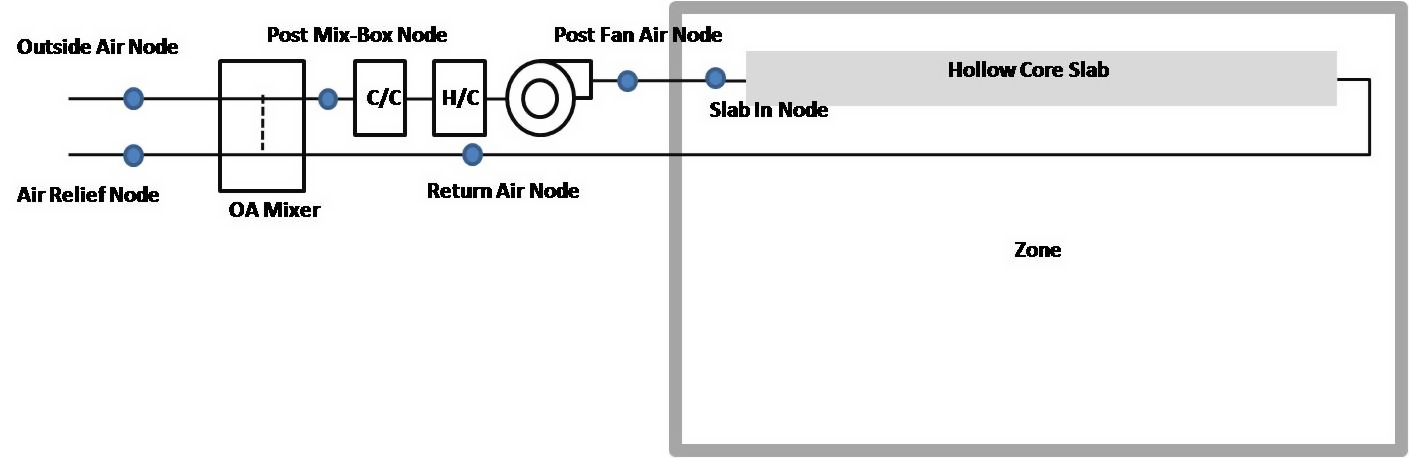
\includegraphics[width=0.9\textwidth, height=0.9\textheight, keepaspectratio=true]{media/image321.png}
\caption{Ventilated Slab model - basic system \protect \label{fig:ventilated-slab-model-basic-system}}
\end{figure}

\subsubsection{Inputs}\label{inputs-10-014}

\paragraph{Field: Name}\label{field-name-10-012}

This field is a unique user assigned name for an instance of a ventilated slab system. Any reference to this unit by another object will use this name. Other objects that use this ventilated slab system will reference it by this name.

\paragraph{Field: Availability Schedule Name}\label{field-availability-schedule-name-9-001}

This field is the name of the schedule (ref: Schedule) that denotes whether the ventilated slab system can run during a given time period. A schedule value less than or equal to 0 (usually 0 is used) denotes that the unit must be off for that time period. A value greater than 0 (usually 1 is used) denotes that the unit is available to operate during that time period. If this field is left blank, the schedule has a value of 1 for all time periods.

\begin{figure}[hbtp] % fig 129
\centering
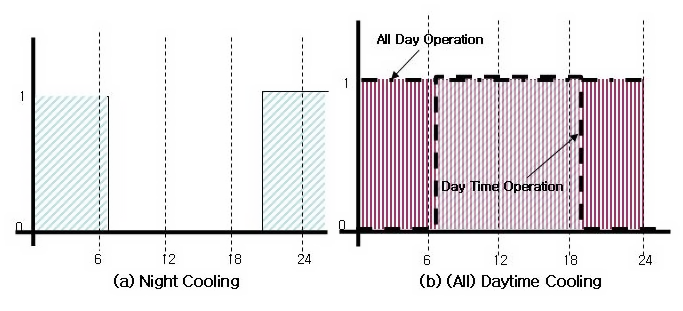
\includegraphics[width=0.9\textwidth, height=0.9\textheight, keepaspectratio=true]{media/image322.png}
\caption{Example operating schedule for Ventilated Slab \protect \label{fig:example-operating-schedule-for-ventilated}}
\end{figure}

\paragraph{Field: Zone Name}\label{field-zone-name-4-004}

This field is the name of the zone (Ref: Zone) in which the ventilated slab system is principally located and intended to affect. A system that is between two zones will still act upon each zone; however, the zone name referenced here should be the zone that controls the system response.

\paragraph{Field: Surface Name or Radiant Surface Group Name}\label{field-surface-name-or-radiant-surface-group-name-3}

This field is the name of the surface (Ref: Surface) or surface list (Ref: \hyperref[zonehvacventilatedslabslabgroup]{ZoneHVAC:VentilatedSlab:SlabGroup}) in which the hollow cores are embedded/contained. This specification attaches the source or sinks from the radiant system to a particular surface and the contribution of the system to the heat balances of that surface. If this field is a surface list, then the source or sink is attached to all of the surfaces in the list with the radiant system surface group defining the breakdown of how flow rate is split between the various surfaces. Only base surfaces (Walls, Roofs, Floors) are valid. Window/Door surfaces and Internal Mass are not valid surface types for embedded radiant systems.

\paragraph{Field: Maximum Air Flow Rate}\label{field-maximum-air-flow-rate-001}

This field allows the user to enter the maximum volumetric flow rate of air through the ventilated slab system in m\(^{3}\)/sec.~ This parameter should be some real number greater than zero.

\paragraph{Field: Outdoor Air Control Type}\label{field-outdoor-air-control-type}

This field allows the user to control how outdoor air is used in the ventilated slab system.~ The ventilated slab system described by this syntax has its own outdoor air handler.~ The three options for outdoor air control are ``\textbf{VariablePercent}'', ``\textbf{FixedTemperature}'' and ``\textbf{FixedAmount}''. Those keywords are the only allowed choices for this parameter.~ In general, the variable percent control will attempt to vary the amount of outdoor air between some minimum and maximum schedules of fractions (see next two fields) to best meet the current heating or cooling load. The fixed temperature control will vary the amount of outdoor air between the minimum schedule (fraction of maximum, see next field) and 100\% available outdoor air to come as close as possible to a desired mixed air temperature (see two fields down) that can be scheduled. The fixed amount control will fix the outdoor air flow rate as minimum outdoor air flow rate and schedule specified by the user and automatically set the maximum and minimum outside flow rate to be equal by ignoring the maximum outdoor air flow rate. More information on the controls and operation of the ventilated slab are given in the section above (preceding the IDF description).

\paragraph{Field: Minimum Outdoor Air Flow Rate}\label{field-minimum-outdoor-air-flow-rate-001}

This field allows the user to enter the minimum volumetric flow rate of outdoor air (in m\(^{3}\)/sec) that will be brought in to the ventilated slab. The actual minimum outdoor air flow rate will be this number multiplied by the schedule value from the minimum outdoor air schedule. If ``FixedAmount'' type is selected as the outdoor air control strategy, the outdoor air flow rate will be fixed at the value of this field and the ventilated slab will automatically set the maximum and minimum outside flow rate to be equal by ignoring the maximum outdoor air flow rate.

\paragraph{Field: Minimum Outdoor Air Schedule Name}\label{field-minimum-outdoor-air-schedule-name-001}

This field contains a schedule name (ref: Schedule) that should contain values for the minimum outdoor air used by the ventilated slab system for IAQ or other reasons.~ Note that if the ventilated slab is scheduled off or if there is no load sensed in the zone that the system will not operate even to achieve the minimum air fraction.~ However, if the system is operating, it will always bring in at least this fraction of the minimum air flow rate (see minimum air flow rate field above). If ``FixedAmount'' type is selected as the outdoor air control strategy, the actual outdoor air flow rate will be this number multiplied by the minimum outdoor air flow rate in the field above. The ventilated slab will automatically set the maximum and minimum outdoor air schedule to be equal by ignoring the maximum outdoor air schedule.

\paragraph{Field: Maximum Outdoor Air Flow Rate}\label{field-maximum-outdoor-air-flow-rate-001}

This field allows the user to enter the maximum volumetric flow rate of outdoor air that can be brought into the ventilated slab in m\(^{3}\)/sec.~ This parameter should be some real number greater than zero.~ Note that the value for this parameter may be less than the maximum air flow rate of the ventilated slab and this may affect the maximum fraction of outdoor air within the control strategy defined above. This parameter is an absolute maximum and will supercede any scheduled fraction of the ventilated slab maximum airflow rate. If ``FixedAmount'' type is selected as the outdoor air control strategy, this field will be ignored and be automatically set to be equal to the minimum outdoor air flow rate specified in the field above.

\paragraph{Field: Maximum Outdoor Air Fraction or Temperature Schedule Name}\label{field-maximum-outdoor-air-fraction-or-temperature-schedule-name}

This field can have one of two meanings depending the type of control selected in the outdoor air control type parameter above.~ If ``VariablePercent'' or ``FixedAmount'' was selected, then this field is a schedule name (ref: Schedule) corresponding to a maximum air fraction schedule. Furthermore, if ``FixedAmount'' type is selected as the outdoor air control strategy, this field will be ignored and be automatically set to be equal to the minimum outdoor air fraction specified in the field below. Note that this is a fraction of the maximum airflow rate field (see parameter above) for the ventilated slab. If ``FixedTemperature'' control was selected, then this field is still a schedule name (ref: Schedule), but it corresponds to a schedule of mixed air temperatures that the outdoor air control will try to attain.

\paragraph{Field: System Configuration Type}\label{field-system-configuration-type}

This field allows the user to control how the air is circulated using the ventilated slab system.~ The options for system configuration are

\begin{itemize}
\item
  SlabOnly
\item
  SlabAndZone
\item
  SeriesSlabs
\end{itemize}

In the \textbf{SlabOnly}, the ventilation air is sent to the slab only and does not enter the zone.~ In the \textbf{SlabAndZone}, the air first enters the slab and then is delivered to the zone before returning to the system. With the \textbf{SeriesSlabs} option, the user specifies a list of slabs (\hyperref[zonehvacventilatedslabslabgroup]{ZoneHVAC:VentilatedSlab:SlabGroup}). This list determines the order of slabs through which the air passes.~ In this option, air is not delivered to any zone.

\paragraph{Field: Hollow Core Inside Diameter}\label{field-hollow-core-inside-diameter}

This field is the inside diameter of the cores through which air is circulated for the system being defined by this statement.~ The inside diameter should be recorded in meters and is used to determine the convective heat transfer from the circulated air to the inside surface of the ventilated slab.

\paragraph{Field: Hollow Core Length}\label{field-hollow-core-length}

This field is the length of core embedded in the surface named above in the surface name field.~ In other words, this should be the distance that air travels as it through the slab.~ The length of the hollow core in the slab should be entered in meters and is used to determine the effectiveness of heat transfer from the air being circulated through the cores and the core inside surface.~ Longer core lengths result in more heat transferred to/from the radiant surface to the circulating fluid.

\paragraph{Field: Number of Cores}\label{field-number-of-cores}

This field allows the user to specify how many cores there are in the ventilated slab.~ Air flow will be divided equally among the different cores.

\paragraph{Field: Temperature Control Type}\label{field-temperature-control-type-4}

This field specifies along with the throttling range and setpoint schedules how the user wishes to control the ventilated slab system.~ The temperature denoted in the set temperature schedule can refer to one of seven different temperatures: the zone mean air temperature, the zone mean radiant temperature, the zone operative temperature, the surface temperature of the ventilated slab, the outdoor dry-bulb temperature, the outdoor wet-bulb temperature, or the dewpoint temperature of zone mean air temperature.~ The choice of temperature is controlled by the current field---temperature control type.~ The user must select from the following options:

\begin{itemize}
\item
  MeanAirTemperature
\item
  MeanRadiantTemperature
\item
  OperativeTemperature
\item
  OutdoorDryBulbTemperature
\item
  OutdoorWetBulbTemperature
\item
  SurfaceTemperature
\item
  ZoneAirDewPointTemperature
\end{itemize}

If the user does not select a control type, \textbf{MeanAirTemperature} control is assumed by EnergyPlus. See the control temperature schedule fields below for more information.

\paragraph{Field: Heating High Air Temperature Schedule Name}\label{field-heating-high-air-temperature-schedule-name}

This field specifies the high air temperature in degrees Celsius for the temperature control of a ventilated slab system. Air and control temperatures for heating work together to provide a linear function that determines the air temperature sent to the ventilated slab. The current control temperature (see Temperature Control Type above) is compared to the high and low control temperatures at the current time.~~~~~ If the control temperature is above the high temperature, then the inlet air temperature is set to the low air temperature. If the control temperature is below the low temperature, then the inlet air temperature is set to the high air temperature. If the control temperature is between the high and low value, then the inlet air temperature is linearly interpolated between the low and high air temperature values.

\paragraph{Field: Heating Low Air Temperature Schedule Name}\label{field-heating-low-air-temperature-schedule-name}

This field specifies the low air temperature in degrees Celsius for the temperature control of a ventilated slab. For more information on its interpretation, see Heating High Air Temperature Schedule above.

\paragraph{Field: Heating High Control Temperature Schedule Name}\label{field-heating-high-control-temperature-schedule-name-1}

This field specifies the high control temperature in degrees Celsius for the temperature control of a ventilated slab. For more information on its interpretation, see Heating High Air Temperature Schedule above.

\paragraph{Field: Heating Low Control Temperature Schedule Name}\label{field-heating-low-control-temperature-schedule-name-1}

This field specifies the low control temperature in degrees Celsius for the temperature control of a ventilated slab. For more information on its interpretation, see Heating High Air Temperature Schedule above.

\paragraph{Field: Cooling High Air Temperature Schedule Name}\label{field-cooling-high-air-temperature-schedule-name}

This field specifies the high air temperature in degrees Celsius for the temperature control of a ventilated slab system. Air and control temperatures for cooling work together to provide a linear function that determines the air temperature sent to the ventilated slab system. The current control temperature (see Temperature Control Type above) is compared to the high and low control temperatures at the current time. If the control temperature is above the high temperature, then the inlet air temperature is set to the low air temperature. If the control temperature is below the low temperature, then the inlet air temperature is set to the high air temperature. If the control temperature is between the high and low value, then the inlet air temperature is linearly interpolated between the low and high air temperature values.

\paragraph{Field: Cooling Low Air Temperature Schedule Name}\label{field-cooling-low-air-temperature-schedule-name}

This field specifies the low air temperature in degrees Celsius for the temperature control of a constant flow cooling radiant system. For more information on its interpretation, see Cooling High Air Temperature Schedule above.

\paragraph{Field: Cooling High Control Temperature Schedule Name}\label{field-cooling-high-control-temperature-schedule-name-1}

This field specifies the high control temperature in degrees Celsius for the temperature control of a constant flow cooling radiant system. For more information on its interpretation, see Cooling High Air Temperature Schedule above.

\paragraph{Field: Cooling Low Control Temperature Schedule Name}\label{field-cooling-low-control-temperature-schedule-name-1}

This field specifies the low control temperature in degrees Celsius for the temperature control of a ventilated slab system. For more information on its interpretation, see Cooling High Air Temperature Schedule above.

\paragraph{Field: Return Air Node Name}\label{field-return-air-node-name-000}

This field is a node name used to identify the node that serves as the zone return air inlet to the ventilated slab system. This node is one of the inlets to the outdoor air mixer which is implicit in the ventilated slab system model. For ``SlabAndZone'' configuration, the Return Air Node will typically be the same node as a zone exhaust node. For ``SlabOnly'' or ``SeriesSlabs'' configuration, this node name is required but will have zero flow.

\paragraph{Field: Slab In Node Name}\label{field-slab-in-node-name}

This field is a node name used to identify the node that serves as the inlet of the ventilated slab or series of slabs, after the outdoor air mixer, fan, and optional coils.

\paragraph{Field: Zone Supply Air Node Name}\label{field-zone-supply-air-node-name-000}

This field is a node name used to identify the node that serves as the outlet from the ventilated slab system to the zone when using the ``SlabAndZone'' configuration. It is the node exiting the slab section of the system. This node will typically be the same node as a zone inlet node. In the case of ``SlabOnly'' or ``SeriesSlabs'' configuration, this field will be ignored and it should be left BLANK.

\paragraph{Field: Outdoor Air Node Name}

This field is a node name used to identify the node associated with fresh outdoor air brought into the ventilated slab system outdoor air mixer.~ This node should also be specified in an \hyperref[outdoorairnode]{OutdoorAir:Node} or \hyperref[outdoorairnodelist]{OutdoorAir:NodeList} object.

\paragraph{Field: Relief Air Node Name}\label{field-relief-air-node-name}

This field is a node name used to identify the node associated with air exhausted out of the ventilated slab system to the outdoor environment.

\paragraph{Field: Outdoor Air Mixer Outlet Node Name}\label{field-outdoor-air-mixer-outlet-node-name}

This field is a node name used to identify the node associated with the ``mixed'' air of the ventilated slab.~ These conditions are post-``mixing box'' since they are the conditions of the fraction of return air combined with the outdoor air.~ Since this is a simple system, this can also be viewed as the conditions of the air being sent to the coils.

\paragraph{Field: Fan Outlet Node Name}\label{field-fan-outlet-node-name}

This field is a node name used to identify the node that serves as the air outlet from the fan.

\paragraph{Field: Fan Name}\label{field-fan-name-003}

This field is the name of a fan (ref: \hyperref[fansystemmodel]{Fan:SystemModel} or \hyperref[fanconstantvolume]{Fan:ConstantVolume}) that is part of the ventilated slab system.  This name links the ventilated slab to particular fan data entered elsewhere in the input data file.  A fan name is required since it is the prime mover of air in the ventilated slab system.

\paragraph{Field: Coil Option Type}\label{field-coil-option-type}

This field allows the user to specify the coil operating options as one of the following options:

\begin{itemize}
\item
  None
\item
  Heating
\item
  Cooling
\item
  HeatingAndCooling
\end{itemize}

If \textbf{None} is selected, the ventilated slab does not have any coils, and any other input will be ignored. If either \textbf{Heating} or \textbf{Cooling} is selected, only a heating or cooling coil, respectively, is present.~ Thus, only four more inputs will be expected. If \textbf{HeatingAndCooling} is selected, both heating and cooling coil input must be entered, and the ventilated slab will have both a heating and a cooling coil.

\paragraph{Field: Heating Coil Object Type}\label{field-heating-coil-object-type-001}

This field is the type of coil (ref: \hyperref[coilheatingwater]{Coil:Heating:Water}, \hyperref[coilheatingelectric]{Coil:Heating:Electric}, \hyperref[coilheatinggas-000]{Coil:Heating:Fuel}, \hyperref[coilheatingsteam]{Coil:Heating:Steam}) that is used for heating in the ventilated slab system. This field must be one of the following keywords: \hyperref[coilheatingwater]{Coil:Heating:Water}, \hyperref[coilheatingelectric]{Coil:Heating:Electric}, \hyperref[coilheatinggas-000]{Coil:Heating:Fuel}, \hyperref[coilheatingsteam]{Coil:Heating:Steam}.~ It is used in conjunction with the heating coil name (see next field) to specify the heating coil present within the system.

\paragraph{Field: Heating Coil Name}\label{field-heating-coil-name-001}

This field is the name of the heating coil that is part of the ventilated slab system.~ It is assumed that there is always some sort of heating coil associated with a ventilated slab system.~ This name links the ventilated slab to particular heating coil data entered elsewhere in the input data file.

\paragraph{Field: Hot Water or Steam Inlet Node Name}\label{field-hot-water-or-steam-inlet-node-name}

This field corresponds to the water inlet node to the heating coil for a water coil.~ The water inlet node controls how a water heating coil operates.~ This field is ignored/not needed for gas and electric heating coils.

\paragraph{Field: Cooling Coil Object Type}\label{field-cooling-coil-object-type-001}

This field is the name of the cooling coil (ref: \hyperref[coilcoolingwater]{Coil:Cooling:Water}, \hyperref[coilcoolingwaterdetailedgeometry]{Coil:Cooling:Water:DetailedGeometry}, \hyperref[coilsystemcoolingwaterheatexchangerassisted]{CoilSystem:Cooling:Water:HeatExchangerAssisted}) that is part of the ventilated slab system.~ This name links the ventilated slab system to particular cooling coil data entered elsewhere in the input data file. If no cooling coil is present, the previous field may be followed by a semi-colon and the remaining parameters in this statement may be ignored.

\paragraph{Field: Cooling Coil Name}\label{field-cooling-coil-name-001}

This field is the name of the cooling coil that is part of the ventilated slab system.~ It is assumed that there is always some sort of cooling coil associated with a ventilated slab system.~ This name links the ventilated slab to particular cooling coil data entered elsewhere in the input data file.

\paragraph{Field: Cold Water Inlet Node Name}\label{field-cold-water-inlet-node-name}

This field corresponds to the water inlet node to the cooling coil.~ The water inlet node controls how a water cooling coil operates and is required for the ventilated slab system that has a cooling coil associated with it to function properly.

\paragraph{Field: Availability Manager List Name}\label{field-availability-manager-list-name-001}

This optional input field is the name of an \hyperref[availabilitymanagerassignmentlist]{AvailabilityManagerAssignmentList} object. An Availability Manager Assignment List is a list of Availability Managers giving both Availability Manager type and name. The availability managers in the list apply to this ventilated slab object's fan. If the ventilated slab is available (per the Availability Schedule Name input field above) and this input field has a valid availability manager assignment list name, then the availability managers in the list determine when and if the fan of this ventilated slab object should be on or off.

\paragraph{Field: Design Specification ZoneHVAC Sizing Object Name}\label{field-design-specification-zonehvac-sizing-object-name}

This optional input field is the name of a \hyperref[designspecificationzonehvacsizing]{DesignSpecification:ZoneHVAC:Sizing} object. The name must correspond to unique name of a \hyperref[designspecificationzonehvacsizing]{DesignSpecification:ZoneHVAC:Sizing} object. A Design Sepcification Zone HVAC Sizing object defines scalable sizing methods for sizing input fields such as Maximum Air Flow Rate in this Ventilated Slab zone HVAC object. The scaled Maximum Air Flow Rate in turn is used to size cooling and heating capacity of the coils.

An example IDF with a ventilated slab is shown below.

\begin{lstlisting}

  ZoneHVAC:VentilatedSlab,
      Zone4VentSlab,           !- Name
      VentSlabAvailability,    !- Availability Schedule Name
      SPACE4-1,                !- Zone Name
      F4-1,                    !- Surface Name or Radiant Surface Group Name
      0.84,                    !- Maximum Air Flow Rate {m3/s}
      VariablePercent,         !- Outdoor Air Control Type
      0.168,                   !- Minimum Outdoor Air Flow Rate {m3/s}
      U2MinOASched,            !- Minimum Outdoor Air Schedule Name
      0.84,                    !- Maximum Outdoor Air Flow Rate {m3/s}
      VentSlabMaxOA,           !- Maximum Outdoor Air Fraction or Temperature Schedule Name
      SlabAndZone,             !- System Configuration Type
      0.050,                   !- Hollow Core Inside Diameter {m}
      15.0,                    !- Hollow Core Length {m}
      50.0,                    !- Number of Cores
      MeanRadiantTemperature,  !- Temperature Control Type
      VentSlabHotHighAir,      !- Heating High Air Temperature Schedule Name
      VentSlabHotLowAir,       !- Heating Low Air Temperature Schedule Name
      VentSlabHotHighControl,  !- Heating High Control Temperature Schedule Name
      VentSlabHotLowControl,   !- Heating Low Control Temperature Schedule Name
      VentSlabCoolHighAir,     !- Cooling High Air Temperature Schedule Name
      VentSlabCoolLowAir,      !- Cooling Low Air Temperature Schedule Name
      VentSlabCoolHighControl, !- Cooling High Control Temperature Schedule Name
      VentSlabCoolLowControl,  !- Cooling Low Control Temperature Schedule Name
      Zone4VentSlabReturnAirNode,  !- Return Air Node Name
      Zone4VentslabSlabInNode, !- Slab In Node Name
      Zone4Inlets,             !-Zone Supply Air Node Name
      Zone4VentSlabOAInNode,   !- Outdoor Air Node Name
      Zone4VentSlabExhNode,    !- Relief Air Node Name
      Zone4VentSlabOAMixerOutletNode,  !-Outdoor Air Mixer Outlet Node Name
      Zone4VentSlabFanOutletNode,  !- Fan Outlet Node Name
      Zone4VentSlabFan,        !- Fan Name
      HeatingAndCooling,       !- Coil Option Type
      Coil:Heating:Electric,   !- Heating Coil Object Type
      Zone4VentSlabHeatingCoil,!- Heating Coil Name
      ,                        !- Hot Water or Steam Inlet Node Name
      Coil:Cooling:Water,      !- Cooling Coil Object Type
      Zone4VentSlabCoolingCoil,!- Cooling Coil Name
      Zone4VentSlabChWInletNode;  !- Cold Water Inlet Node Name
\end{lstlisting}

\subsubsection{Outputs}\label{outputs-9-006}

\begin{itemize}
\item
  HVAC,Average,Zone Ventilated Slab Radiant Heating Rate {[}W{]}
\item
  HVAC,Sum,Zone Ventilated Slab Radiant Heating Energy {[}J{]}
\item
  HVAC,Average,Zone Ventilated Slab Radiant Cooling Rate {[}W{]}
\item
  HVAC,Sum,Zone Ventilated Slab Radiant Cooling Energy {[}J{]}
\item
  HVAC,Average,Zone Ventilated Slab Coil Heating Rate {[}W{]}
\item
  HVAC,Sum,Zone Ventilated Slab Coil Heating Energy {[}J{]}
\item
  HVAC,Average,Zone Ventilated Slab Coil Total Cooling Rate {[}W{]}
\item
  HVAC,Sum,Zone Ventilated Slab Coil Total Cooling Energy {[}J{]}
\item
  HVAC,Average,Zone Ventilated Slab Coil Sensible Cooling Rate {[}W{]}
\item
  HVAC,Sum,Zone Ventilated Slab Coil Sensible Cooling Energy {[}J{]}
\item
  HVAC,Average,Zone Ventilated Slab Coil Latent Cooling Rate {[}W{]}
\item
  HVAC,Sum,Zone Ventilated Slab Coil Latent Cooling Energy {[}J{]}
\item
  HVAC,Average, Zone Ventilated Slab Air Mass Flow Rate {[}kg/s{]}
\item
  HVAC,Average, Zone Ventilated Slab Fan Electricity Rate {[}W{]}
\item
  HVAC,Sum,Zone Ventilated Slab Fan Electricity Energy {[}J{]}
\item
  HVAC,Average,Zone Ventilated Slab Inlet Air Temperature {[}C{]}
\item
  HVAC,Average,Zone Ventilated Slab Outlet Air Temperature {[}C{]}
\item
  HVAC,Average,Zone Ventilated Slab Zone Inlet Air Temperature {[}C{]}
\item
  HVAC,Average,Zone Ventilated Slab Return Air Temperature {[}C{]}
\item
  HVAC,Average,Zone Ventilated Slab Fan Outlet Air Temperature {[}C{]}
\item
  HVAC,Average,Zone Ventilated Slab Fan Availability Status {[]}
\end{itemize}

\paragraph{Zone Ventilated Slab Radiant Heating Rate~ {[}W{]}}\label{zone-ventilated-slab-radiant-heating-rate-w}

This field reports the radiant heating input rate of the ventilated slab system to the zone it is serving in Watts.~ This is determined by outlet and zone air conditions and the mass flow rate through the ventilated slab system.

\paragraph{Zone Ventilated Slab Radiant Heating Energy {[}J{]}}\label{zone-ventilated-slab-radiant-heating-energy-j}

This field is the heating radiant input of the ventilated slab system to the zone it is serving in Joules over the timestep being reported.~ This is determined by outlet and zone air conditions, the mass flow rate through the ventilated slab system, and the timestep.

\paragraph{Zone Ventilated Slab Radiant Cooling Rate {[}W{]}}\label{zone-ventilated-slab-radiant-cooling-rate-w}

This field reports the radiant cooling input rate to the ventilated slab system in Watts. This is the heat sink to the surface that is defined as the ventilated slab system. The cooling rate is determined by the zone conditions and the control scheme defined in the user input.

\paragraph{Zone Ventilated Slab Radiant Cooling Energy {[}J{]}}\label{zone-ventilated-slab-radiant-cooling-energy-j}

This field reports the radiant cooling input to the ventilated slab system in Joules. This is the heat sink to the surface that is defined as the radiant system. The cooling rate is determined by the zone conditions, the control scheme defined in the user input, and the timestep.

\paragraph{Zone Ventilated Slab Coil Heating Rate {[}W{]}}\label{zone-ventilated-slab-coil-heating-rate-w}

This field reports the heating input rate of the heating coil of ventilated slab system the zone it is serving in Watts.~ This is determined by return air and zone air conditions and the mass flow rate through the ventilation slab system.

\paragraph{Zone Ventilated Slab Coil Heating Energy {[}J{]}}\label{zone-ventilated-slab-coil-heating-energy-j}

This field is the heating output of the heating coil of the ventilated slab system the zone it is serving in Joules over the timestep being reported.~ This is determined by return air and zone air conditions, the mass flow rate through the ventilation slab system, and the timestep.

\paragraph{Zone Ventilated Slab Coil Total Cooling Rate {[}W{]}}\label{zone-ventilated-slab-coil-total-cooling-rate-w}

This field reports the total cooling (sensible plus latent) output rate of the cooling coil of the ventilated slab system to the zone it is serving in Watts.~ This is determined by outlet and zone air conditions and the mass flow rate through the ventilation slab system.

\paragraph{Zone Ventilated Slab Coil Total Cooling Energy {[}J{]}}\label{zone-ventilated-slab-coil-total-cooling-energy-j}

This field is the total cooling (sensible plus latent) output of the cooling coil of the ventilated slab system to the zone it is serving in Joules over the timestep being reported.~ This is determined by outlet and zone air conditions, the mass flow rate through the ventilation slab system, and the timestep.

\paragraph{Zone Ventilated Slab Coil Sensible Cooling Rate {[}W{]}}\label{zone-ventilated-slab-coil-sensible-cooling-rate-w}

This field reports the sensible cooling output rate of the cooling coil of the ventilated slab system to the zone it is serving in Watts.~ This is determined by outlet and zone air conditions and the mass flow rate through the ventilation slab system.

\paragraph{Zone Ventilated Slab Coil Sensible Cooling Energy {[}J{]}}\label{zone-ventilated-slab-coil-sensible-cooling-energy-j}

This field is the sensible cooling output of the cooling coli of the ventilated slab system to the zone it is serving in Joules over the timestep being reported.~ This is determined by outlet and zone air conditions, the mass flow rate through the ventilation slab system, and the timestep.

\paragraph{Zone Ventilated Slab Coil Latent Cooling Rate {[}W{]}}\label{zone-ventilated-slab-coil-latent-cooling-rate-w}

This field reports the latent cooling output rate of the cooling coil of the ventilated slab system to the zone it is serving in Watts.~ This is determined by outlet and zone air conditions and the mass flow rate through the ventilation slab system.

\paragraph{Zone Ventilated Slab Coil Latent Cooling Energy {[}J{]}}\label{zone-ventilated-slab-coil-latent-cooling-energy-j}

This field is the latent cooling output of the cooling coli of the ventilated slab system to the zone it is serving in Joules over the timestep being reported.~ This is determined by outlet and zone air conditions, the mass flow rate through the ventilation slab system, and the timestep.

\paragraph{Zone Ventilated Slab Air Mass Flow Rate {[}kg/s{]}}\label{zone-ventilated-slab-air-mass-flow-rate-kgs}

This field reports the mass flow rate of air through the ventilated slab system in kilograms per second.

\paragraph{Zone Ventilated Slab Fan Electricity Rate {[}W{]}}\label{zone-ventilated-slab-fan-electric-power-w}

This field reports the electric power consumption rate of the fan of the ventilated slab system in Watts.

\paragraph{Zone Ventilated Slab Fan Electricity Energy {[}J{]}}\label{zone-ventilated-slab-fan-electric-energy-j}

This field reports the electric power consumed by the fan of the ventilated slab system over the timestep in Joules.

\paragraph{Zone Ventilated Slab Inlet Air Temperature {[}C{]}}\label{zone-ventilated-slab-inlet-air-temperature-c}

This field reports the temperature of air entering the ventilated slab system in Celsius.

\paragraph{Zone Ventilated Slab Outlet Air Temperature {[}C{]}}\label{zone-ventilated-slab-outlet-air-temperature-c}

This field reports the temperature of air leaving the ventilated slab system in Celsius.

\paragraph{Zone Ventilated Slab Zone Inlet Air Temperature {[}C{]}}\label{zone-ventilated-slab-zone-inlet-air-temperature-c}

This field reports the temperature of air entering the zone in Celsius.

\paragraph{Zone Ventilated Slab Return Air Temperature {[}C{]}}\label{zone-ventilated-slab-return-air-temperature-c}

This field reports the temperature of air leaving the zone in Celsius. When system does not circulate air to zone(``SlabOnly'' Configuration), the slab outlet temperature and return air temperature will be the same.

\paragraph{Zone Ventilated Slab Fan Outlet Air Temperature {[}C{]}}\label{zone-ventilated-slab-fan-outlet-air-temperature-c}

This field reports the fan outlet air temperature for the ventilated slab system in Celsius.

\paragraph{Zone Ventilated Slab Fan Availability Status {[]}}\label{zone-ventilated-slab-fan-availability-status}

This is the availability status of the ventilated slab fan. This status flag is a result of the calculations made by the Availability Manager(s) listed in an AvailabilityManagerAssignmentList object and/or calculations made by Hybrid Ventilation Manager object. The AvailabilityManagerAssignmentList is an optional input in the ventilated slab object. When a single availability manager is used in an Availability Manager Assignment List, this is also the availability status reported by the specific availability manager (Ref. AvailabilityManager:* Outputs). For multiple availability managers in an Availability Manager Assignment List along with Hybrid Ventilation Manager, rules to determine fan availability status are described in the section `Group -- System Availability Managers'. The control status outputs are represented using integers 0 through 3. These integers represent NoAction (0), ForceOff (1), CycleOn (2), and CycleOnZoneFansOnly (3). Since the status output is averaged, the output result may not correspond to the values described here when output variable frequencies other than detailed are used. Use the ``detailed'' reporting frequency (Ref. Output:Variable object) to view the availability status at each simulation timestep.

\subsection{ZoneHVAC:VentilatedSlab:SlabGroup}\label{zonehvacventilatedslabslabgroup}

A ventilated slab system may consist of multiple active slabs that are serving to condition the zone. Slabs that act serially can be specified as multiple radiant systems using the standard ventilated slab input described above. This list of surfaces (the name it is assigned) replaces the name of a single surface in the ventilated slab system input described above.

\subsubsection{Inputs}\label{inputs-11-013}

\paragraph{Field : Name of Ventilated Slab Surface Group}\label{field-name-of-ventilated-slab-surface-group}

This field is a unique user assigned name for the list of surfaces that are acting in coordination with one another. Any reference to this list by a ventilated slab system will use this name.

\paragraph{Field: Zone Name}\label{field-zone-name-5-003}

This field is the name of the zone in which the surface is principally located and intended to affect.

\paragraph{Field: Surface Name}\label{field-surface-name-003}

This field is the name of a surface in the zone being conditioned by the ventilated slab system. Only base surfaces like walls, floors and roofs are valid. Door/Window Surface and Internal Mass are not valid surface types for the ventilated slab system.

\paragraph{Field: Core Diameter}\label{field-core-diameter}

This field is the inside diameter of the cores through which air is circulated for the surface being defined by this statement.~ The inside diameter should be recorded in meters and is used to determine the convective heat transfer from the circulated air to the inside surface of the ventilated slab.

\paragraph{Field: Core length}\label{field-core-length}

This field is the length of core embedded in the surface named above in the surface name field.~ In other words, this should be the distance that air travels as it through the slab.~ The length of the hollow core in the surface should be entered in meters and is used to determine the effectiveness of heat transfer from the air being circulated through the cores and the core inside surface.~ Longer core lengths result in more heat transferred to/from the radiant surface to the circulating fluid.

\paragraph{Field: Number of Cores}\label{field-number-of-cores-1}

This field allows the user to specify how many cores there are in the ventilated slab.~ Air flow will be divided equally among the different cores.

\paragraph{Field: Slab Inlet Node Name}\label{field-slab-inlet-node-name}

This field is a node name (character string) used to identify the node that serves as the inlet (air side) to the surface.~ In EnergyPlus, nodes represent points between components or at various points in the loops.~ While a node name may be referenced more than once in an input data file, each node must have a unique name.

\paragraph{Field: Slab Outlet Node Name}\label{field-slab-outlet-node-name}

This field is a node name (character string) used to identify the node that serves as the outlet (air side) of the surface.~ In EnergyPlus, nodes represent points between components or at various points in the loops.~ While a node name may be referenced more than once in an input data file, each node must have a unique name.

An Example IDF with a ventilated slab system is shown below

\begin{lstlisting}

ZoneHVAC:VentilatedSlab:SlabGroup,
      Z125,                    !- Name
      SPACE1-1,                !- Zone 1 Name
      C1-1,                    !- Surface 1 Name
      0.05,                    !- Core Diameter for Surface 1
      30,                      !- Core Length for Surface 1
      20,                      !- Core Numbers for Surface 1
      Z1VentslabIn,            !- Slab In Node Name for Surface 1
      Z1VentSlabout,           !- Slab Outlet Node Name for Surface 1
      SPACE2-1,                !- Zone 2 Name
      C2-1,                    !- Surface 2 Name
      0.05,                    !- Core Diameter for Surface 2
      15,                      !- Core Length for Surface 2
      20,                      !- Core Numbers for Surface 2
      Z2VentSlabIn,            !- Slab In Node Name for Surface 2
      Z2VentSlabOut,           !- Slab Outlet Node Name for Surface 2
      SPACE5-1,                !- Zone 3 Name
      C5-1,                    !- Surface 3 Name
      0.05,                    !- Core Diameter for Surface 3
      30,                      !- Core Length for Surface 3
      20,                      !- Core Numbers for Surface 3
      Z5VentSlabIn,            !- Slab In Node Name for Surface 3
      Z5VentSlabOut;           !- Slab Outlet Node Name for Surface 3
\end{lstlisting}
